% Options for packages loaded elsewhere
\PassOptionsToPackage{unicode}{hyperref}
\PassOptionsToPackage{hyphens}{url}
%
\documentclass[
]{book}
\usepackage{amsmath,amssymb}
\usepackage{lmodern}
\usepackage{ifxetex,ifluatex}
\ifnum 0\ifxetex 1\fi\ifluatex 1\fi=0 % if pdftex
  \usepackage[T1]{fontenc}
  \usepackage[utf8]{inputenc}
  \usepackage{textcomp} % provide euro and other symbols
\else % if luatex or xetex
  \usepackage{unicode-math}
  \defaultfontfeatures{Scale=MatchLowercase}
  \defaultfontfeatures[\rmfamily]{Ligatures=TeX,Scale=1}
\fi
% Use upquote if available, for straight quotes in verbatim environments
\IfFileExists{upquote.sty}{\usepackage{upquote}}{}
\IfFileExists{microtype.sty}{% use microtype if available
  \usepackage[]{microtype}
  \UseMicrotypeSet[protrusion]{basicmath} % disable protrusion for tt fonts
}{}
\makeatletter
\@ifundefined{KOMAClassName}{% if non-KOMA class
  \IfFileExists{parskip.sty}{%
    \usepackage{parskip}
  }{% else
    \setlength{\parindent}{0pt}
    \setlength{\parskip}{6pt plus 2pt minus 1pt}}
}{% if KOMA class
  \KOMAoptions{parskip=half}}
\makeatother
\usepackage{xcolor}
\IfFileExists{xurl.sty}{\usepackage{xurl}}{} % add URL line breaks if available
\IfFileExists{bookmark.sty}{\usepackage{bookmark}}{\usepackage{hyperref}}
\hypersetup{
  pdftitle={2021 연구데이터 분석과정},
  pdfauthor={한국생명공학연구원 김하성},
  hidelinks,
  pdfcreator={LaTeX via pandoc}}
\urlstyle{same} % disable monospaced font for URLs
\usepackage{color}
\usepackage{fancyvrb}
\newcommand{\VerbBar}{|}
\newcommand{\VERB}{\Verb[commandchars=\\\{\}]}
\DefineVerbatimEnvironment{Highlighting}{Verbatim}{commandchars=\\\{\}}
% Add ',fontsize=\small' for more characters per line
\usepackage{framed}
\definecolor{shadecolor}{RGB}{248,248,248}
\newenvironment{Shaded}{\begin{snugshade}}{\end{snugshade}}
\newcommand{\AlertTok}[1]{\textcolor[rgb]{0.94,0.16,0.16}{#1}}
\newcommand{\AnnotationTok}[1]{\textcolor[rgb]{0.56,0.35,0.01}{\textbf{\textit{#1}}}}
\newcommand{\AttributeTok}[1]{\textcolor[rgb]{0.77,0.63,0.00}{#1}}
\newcommand{\BaseNTok}[1]{\textcolor[rgb]{0.00,0.00,0.81}{#1}}
\newcommand{\BuiltInTok}[1]{#1}
\newcommand{\CharTok}[1]{\textcolor[rgb]{0.31,0.60,0.02}{#1}}
\newcommand{\CommentTok}[1]{\textcolor[rgb]{0.56,0.35,0.01}{\textit{#1}}}
\newcommand{\CommentVarTok}[1]{\textcolor[rgb]{0.56,0.35,0.01}{\textbf{\textit{#1}}}}
\newcommand{\ConstantTok}[1]{\textcolor[rgb]{0.00,0.00,0.00}{#1}}
\newcommand{\ControlFlowTok}[1]{\textcolor[rgb]{0.13,0.29,0.53}{\textbf{#1}}}
\newcommand{\DataTypeTok}[1]{\textcolor[rgb]{0.13,0.29,0.53}{#1}}
\newcommand{\DecValTok}[1]{\textcolor[rgb]{0.00,0.00,0.81}{#1}}
\newcommand{\DocumentationTok}[1]{\textcolor[rgb]{0.56,0.35,0.01}{\textbf{\textit{#1}}}}
\newcommand{\ErrorTok}[1]{\textcolor[rgb]{0.64,0.00,0.00}{\textbf{#1}}}
\newcommand{\ExtensionTok}[1]{#1}
\newcommand{\FloatTok}[1]{\textcolor[rgb]{0.00,0.00,0.81}{#1}}
\newcommand{\FunctionTok}[1]{\textcolor[rgb]{0.00,0.00,0.00}{#1}}
\newcommand{\ImportTok}[1]{#1}
\newcommand{\InformationTok}[1]{\textcolor[rgb]{0.56,0.35,0.01}{\textbf{\textit{#1}}}}
\newcommand{\KeywordTok}[1]{\textcolor[rgb]{0.13,0.29,0.53}{\textbf{#1}}}
\newcommand{\NormalTok}[1]{#1}
\newcommand{\OperatorTok}[1]{\textcolor[rgb]{0.81,0.36,0.00}{\textbf{#1}}}
\newcommand{\OtherTok}[1]{\textcolor[rgb]{0.56,0.35,0.01}{#1}}
\newcommand{\PreprocessorTok}[1]{\textcolor[rgb]{0.56,0.35,0.01}{\textit{#1}}}
\newcommand{\RegionMarkerTok}[1]{#1}
\newcommand{\SpecialCharTok}[1]{\textcolor[rgb]{0.00,0.00,0.00}{#1}}
\newcommand{\SpecialStringTok}[1]{\textcolor[rgb]{0.31,0.60,0.02}{#1}}
\newcommand{\StringTok}[1]{\textcolor[rgb]{0.31,0.60,0.02}{#1}}
\newcommand{\VariableTok}[1]{\textcolor[rgb]{0.00,0.00,0.00}{#1}}
\newcommand{\VerbatimStringTok}[1]{\textcolor[rgb]{0.31,0.60,0.02}{#1}}
\newcommand{\WarningTok}[1]{\textcolor[rgb]{0.56,0.35,0.01}{\textbf{\textit{#1}}}}
\usepackage{longtable,booktabs,array}
\usepackage{calc} % for calculating minipage widths
% Correct order of tables after \paragraph or \subparagraph
\usepackage{etoolbox}
\makeatletter
\patchcmd\longtable{\par}{\if@noskipsec\mbox{}\fi\par}{}{}
\makeatother
% Allow footnotes in longtable head/foot
\IfFileExists{footnotehyper.sty}{\usepackage{footnotehyper}}{\usepackage{footnote}}
\makesavenoteenv{longtable}
\usepackage{graphicx}
\makeatletter
\def\maxwidth{\ifdim\Gin@nat@width>\linewidth\linewidth\else\Gin@nat@width\fi}
\def\maxheight{\ifdim\Gin@nat@height>\textheight\textheight\else\Gin@nat@height\fi}
\makeatother
% Scale images if necessary, so that they will not overflow the page
% margins by default, and it is still possible to overwrite the defaults
% using explicit options in \includegraphics[width, height, ...]{}
\setkeys{Gin}{width=\maxwidth,height=\maxheight,keepaspectratio}
% Set default figure placement to htbp
\makeatletter
\def\fps@figure{htbp}
\makeatother
\setlength{\emergencystretch}{3em} % prevent overfull lines
\providecommand{\tightlist}{%
  \setlength{\itemsep}{0pt}\setlength{\parskip}{0pt}}
\setcounter{secnumdepth}{5}
\usepackage{booktabs}
\usepackage{fontspec}
\setmainfont{NanumGothic}
\usepackage{amssymb}
\usepackage[a4paper,left=15mm,right=15mm,top=10mm,bottom=10mm]{geometry}

\ifluatex
  \usepackage{selnolig}  % disable illegal ligatures
\fi
\usepackage[]{natbib}
\bibliographystyle{apalike}

\title{2021 연구데이터 분석과정}
\usepackage{etoolbox}
\makeatletter
\providecommand{\subtitle}[1]{% add subtitle to \maketitle
  \apptocmd{\@title}{\par {\large #1 \par}}{}{}
}
\makeatother
\subtitle{생명정보학을 위한 R프로그래밍(중급과정)}
\author{한국생명공학연구원 김하성}
\date{2021-06-17}

\begin{document}
\maketitle

{
\setcounter{tocdepth}{1}
\tableofcontents
}
\hypertarget{introduction}{%
\chapter{강의 개요}\label{introduction}}

\begin{itemize}
\tightlist
\item
  장소: 코빅 3층 전산교육장(1304호)
\item
  강사: 한국생명공학연구원 바이오합성연구센터 김하성
\item
  연락처: 042-860-4372, \href{mailto:haseong@kribb.re.kr}{\nolinkurl{haseong@kribb.re.kr}} (생명연 연구동 1143)
\item
  강의자료: \url{https://greendaygh.github.io/KRIBBR2021/}
\end{itemize}

\hypertarget{References_n_books}{%
\section{참고 교제}\label{References_n_books}}

\begin{itemize}
\tightlist
\item
  Using R for Introductory Statistics by John Verzani

  \begin{itemize}
  \tightlist
  \item
    Free version of \href{https://cran.r-project.org/doc/contrib/Verzani-SimpleR.pdf}{1st Edition}
  \item
    \href{https://www.crcpress.com/Using-R-for-Introductory-Statistics-Second-Edition/Verzani/p/book/9781466590731}{Second edition}
  \end{itemize}
\item
  \href{https://r4ds.had.co.nz}{R for Data Science}
\item
  \href{http://2.droppdf.com/files/5aTvl/bioinformatics-data-skills.pdf}{Bioinformatics Data Skills} by Vince Buffalo
\item
  \href{http://www.academia.dk/BiologiskAntropologi/Epidemiologi/PDF/Introductory_Statistics_with_R__2nd_ed.pdf}{Introductory Statistics with R} by Dalgaard
\item
  일반통계학 (영지문화사, 김우철 외)
\end{itemize}

\hypertarget{References}{%
\section{참고 자료}\label{References}}

\begin{itemize}
\tightlist
\item
  \href{https://www.r-project.org/}{R 홈페이지}
\item
  \href{https://www.rstudio.com/}{Rstudio 홈페이지}
\item
  \href{https://www.bioconductor.org/}{Bioconductor}
\item
  \href{https://cran.r-project.org/manuals.html}{R 기본 문서들}
\item
  \href{https://bookdown.org/}{R ebooks}
\item
  \href{https://www.rstudio.com/resources/cheatsheets/}{Cheat Sheets}
\item
  \href{https://resources.rstudio.com/}{RStudio Webinars}
\item
  \href{http://shiny.rstudio.com/tutorial/}{Shiny}
\item
  \href{https://github.com/hadley}{Hadley github}
\end{itemize}

\hypertarget{Schedule}{%
\section{강의 계획}\label{Schedule}}

\begin{itemize}
\tightlist
\item
  Day1 - R, Rstudio Basics, Tindyverse
\item
  Day2 - Bioconductor, Sequence data analysis
\item
  Day3 - High-throughput sequence data
\item
  Day4 - Annotation
\end{itemize}

\hypertarget{rrstudio-basics}{%
\chapter{R/Rstudio basics}\label{rrstudio-basics}}

\hypertarget{what-is-r-rstudio}{%
\section{What is R / Rstudio}\label{what-is-r-rstudio}}


\includegraphics[width=1.04167in,height=\textheight]{images/01/r.jpg}

R은 통계나 생물통계, 유전학을 연구하는 사람들 사이에서 널리 사용되는 오픈소스 프로그래밍 언어 입니다. Bell Lab에서 개발한 S 언어에서 유래했으며 많은 패키지가 (다른 사람들이 만들어 놓은 코드) 있어서 쉽게 가져다 사용할 수 있습니다. R은 복잡한 수식이나 통계 알고리즘을 간단히 구현하고 사용할 수 있으며 C, C++, Python 등 다른 언어들과의 병행 사용도 가능합니다.

R은 통계분석에 널리 사용되는데 이는 데이터 가시화를 위한 그래픽 기능이나 벡터 연산 등의 편리함 때문에 점점 더 많은 사람들이 사용하고 있습니다. 기존에는 느린 속도나 부족한 확장성이 다른 언어들에 비해 단점으로 지적되었으나 R 언어의 계속적인 개발과 업데이트로 이러한 단점들이 빠르게 극복되고 있습니다. R 사용을 위해서는 R 언어의 코어 프로그램을 먼저 설치하고 그 다음 R 언어용 IDE인 RStudio 설치가 필요합니다.

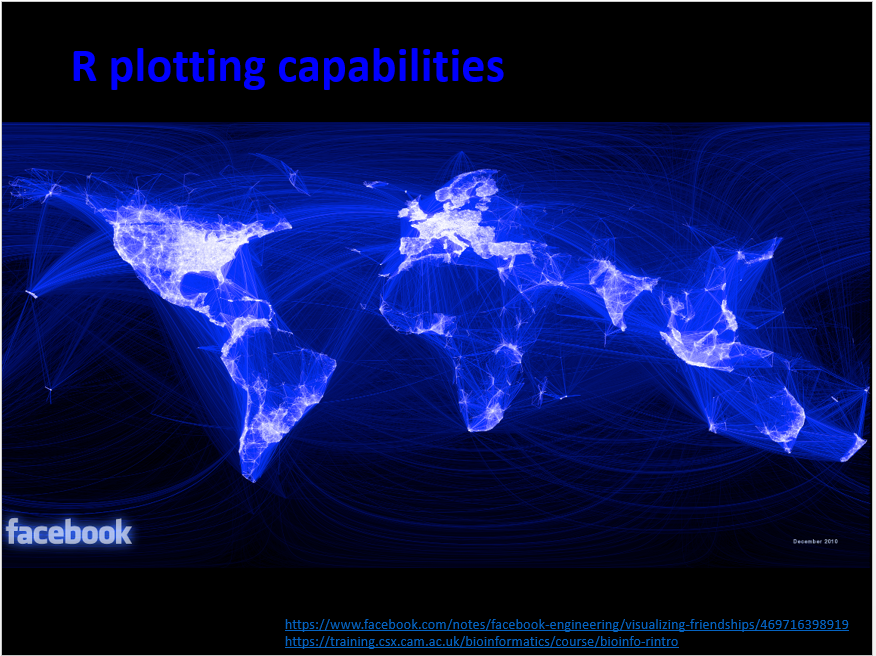
\includegraphics[width=3.125in,height=\textheight]{images/01/22.PNG}
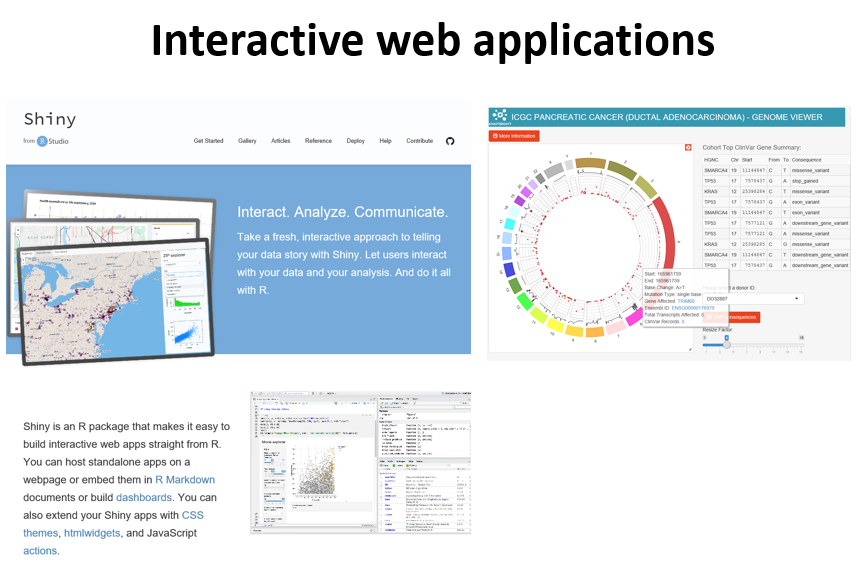
\includegraphics[width=3.125in,height=\textheight]{images/01/23.PNG}

\hypertarget{r-rstudio-installation}{%
\section{R / Rstudio Installation}\label{r-rstudio-installation}}

\hypertarget{r-uxc124uxce58}{%
\subsection{R 설치}\label{r-uxc124uxce58}}

\begin{itemize}
\tightlist
\item
  R 사이트에 접속 후 (\url{https://www.r-project.org/}) 좌측 메뉴 상단에 위치한 CRAN 클릭.
\item
  미러 사이트 목록에서 Korea의 아무 사이트나 들어감
\item
  Download R for Windows를 클릭 후 base 링크 들어가서
\item
  Download R x.x.x for Windows 링크 클릭으로 실행 프로그램 다운로드 - 로컬 컴퓨터에 Download 된 R-x.x.x-win.exe 를 실행
\item
  설치 가이드에 따라 R 언어 소프트웨어 설치 완료
\end{itemize}

\hypertarget{rstudio-uxc124uxce58}{%
\subsection{Rstudio 설치}\label{rstudio-uxc124uxce58}}

Rstudio는 R 언어를 위한 오픈소스 기반 통합개발환경(IDE)으로 R 프로그래밍을 위한 편리한 기능들을 제공해 줍니다.

\begin{itemize}
\tightlist
\item
  사이트에 접속 (\url{https://www.rstudio.com/}), 상단의 Products \textgreater{} RStudio 클릭
\item
  RStudio Desktop 선택
\item
  Download RStudio Desktop 클릭
\item
  RStudio Desktop Free 버전의 Download를 선택하고
\item
  Download RStudio for Windows 클릭, 다운로드
\item
  로컬 컴퓨터에 다운로드된 RStudio-x.x.x.exe 실행
\item
  설치 가이드에 따라 설치 완료
\end{itemize}

\hypertarget{rstudio-interface}{%
\section{Rstudio interface}\label{rstudio-interface}}

\begin{itemize}
\tightlist
\item
  좌측 상단의 공간은 코드편집창, 좌측 하단은 콘솔창 이며 각 위치를 기호에 따라서 바꿀 수 있습니다.
\end{itemize}

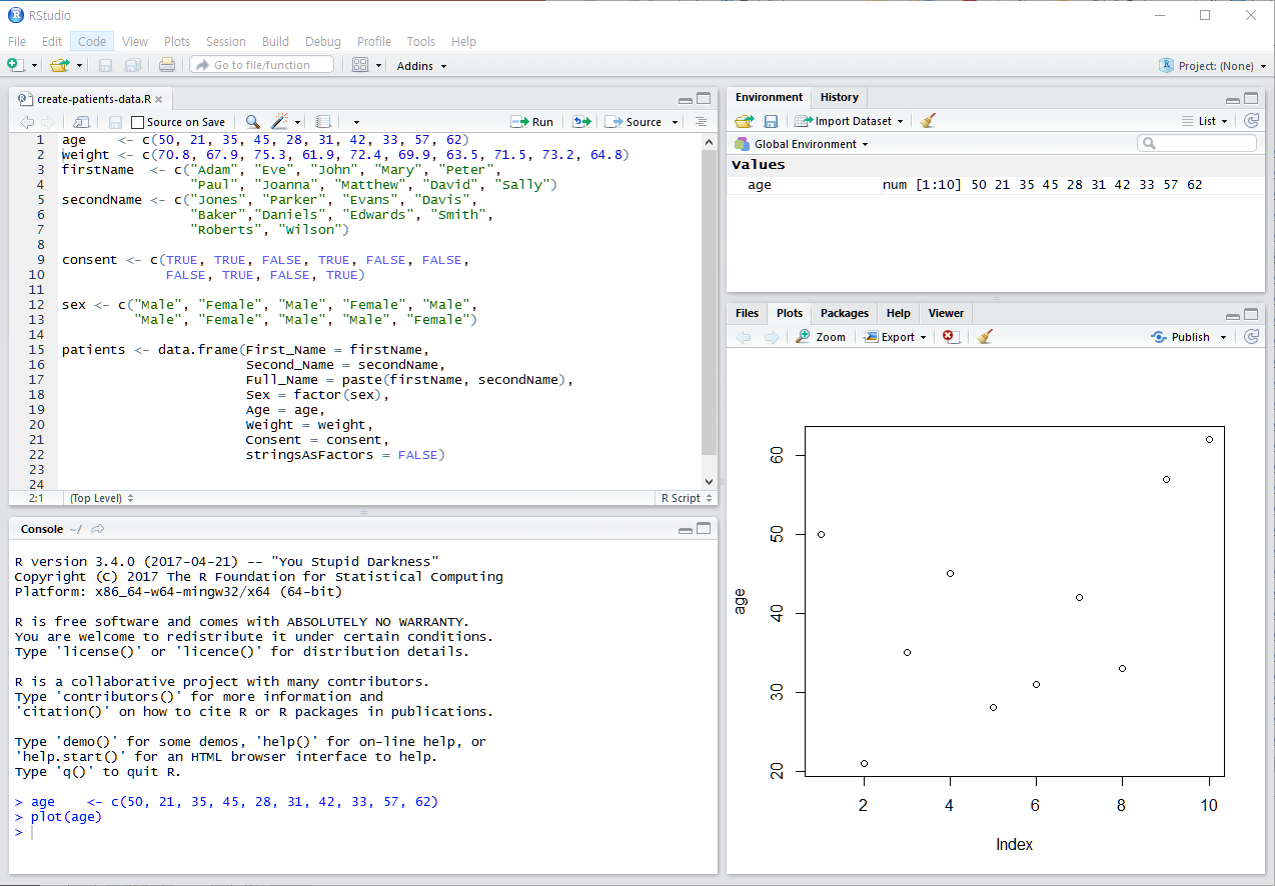
\includegraphics[width=4.16667in,height=\textheight]{images/01/01-11.PNG}

\hypertarget{keyboard-shortcuts}{%
\subsection{Keyboard shortcuts}\label{keyboard-shortcuts}}

\begin{itemize}
\tightlist
\item
  참고사이트

  \begin{itemize}
  \tightlist
  \item
    \url{https://support.rstudio.com/hc/en-us/articles/200711853-Keyboard-Shortcuts}
  \item
    Tools --\textgreater{} Keyboard shortcut Quick Reference (\texttt{Alt\ +\ Shift\ +\ K})
  \end{itemize}
\item
  코드편집창 이동 (\texttt{Ctrl+1}) 콘솔창 이동(\texttt{Ctrl+2})
\item
  한 줄 실행 (\texttt{Ctrl+Enter})
\item
  주석처리 (\texttt{Ctrl\ +\ Shift\ +\ C})

  \begin{itemize}
  \tightlist
  \item
    또는 \texttt{\#}으로 시작하는 라인
  \end{itemize}
\end{itemize}

\hypertarget{exercise}{%
\subsection{Exercise}\label{exercise}}

\begin{enumerate}
\def\labelenumi{\arabic{enumi}.}
\tightlist
\item
  코드편집창에서 다음 입력하시오
\end{enumerate}

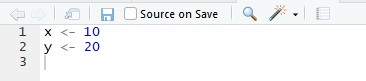
\includegraphics{images/01/01-14.PNG}

\begin{itemize}
\tightlist
\item
  단축키 \texttt{Ctrl\ +\ enter}로 코드 실행
\item
  단축키 \texttt{Ctrl\ +\ 2}로 커서 콘솔창으로 이동
\item
  \texttt{x}값 \texttt{x+y}값 확인
\item
  단축키 \texttt{Ctrl\ +\ 1}로 코드편집창 이동
\item
  단축키 \texttt{Ctrl\ +\ Shift\ +\ C} 사용
\end{itemize}

\begin{Shaded}
\begin{Highlighting}[]
\CommentTok{\# x \textless{}{-} 10}
\CommentTok{\# y \textless{}{-} 20}
\end{Highlighting}
\end{Shaded}

\hypertarget{set-a-project}{%
\subsection{Set a project}\label{set-a-project}}

\begin{itemize}
\item
  프로젝트를 만들어서 사용할 경우 파일이나 디렉토리, 내용 등을 쉽게 구분하여 사용 가능합니다. 아래와 같이 원하는 위치에 원하는 이름의 프로젝트를 생성하고 프로젝트를 시작할 때는 해당 디렉토리의 \texttt{xxx.Rproj} 파일을 클릭합니다.
\item
  File \textgreater{} New Project \textgreater{} New Directory \textgreater{} New Project \textgreater{} ``kribb-R'' \textgreater{} Create Project
\item
  File \textgreater{} New File \textgreater{} R Script \textgreater{} ``day1.R''
\end{itemize}

\hypertarget{r-programming}{%
\section{R programming}\label{r-programming}}

\hypertarget{console-calculator}{%
\subsection{Console calculator}\label{console-calculator}}

\begin{Shaded}
\begin{Highlighting}[]
\DecValTok{2} \SpecialCharTok{+} \DecValTok{2}
\NormalTok{((}\DecValTok{2}\NormalTok{ – }\DecValTok{1}\NormalTok{)}\SpecialCharTok{\^{}}\DecValTok{2} \SpecialCharTok{+}\NormalTok{ (}\DecValTok{1}\NormalTok{ – }\DecValTok{3}\NormalTok{)}\SpecialCharTok{\^{}}\DecValTok{2}\NormalTok{ )}\SpecialCharTok{\^{}}\NormalTok{(}\DecValTok{1}\SpecialCharTok{/}\DecValTok{2}\NormalTok{)}
\DecValTok{2} \SpecialCharTok{+} \DecValTok{2}\NormalTok{; }\DecValTok{2} \SpecialCharTok{{-}} \DecValTok{2}
\end{Highlighting}
\end{Shaded}

\hypertarget{exercise-1}{%
\subsection{Exercise}\label{exercise-1}}

다음 공식들을 계산하는 R 코드를 작성하시오

\[ \sqrt{(4+3)(2+1)} \]

\[ 2^3 + 3^2 \]

\[ \frac{0.25 - 0.2}{\sqrt{0.2 (1-0.2)/100}}\]

\hypertarget{variables-and-values}{%
\subsection{Variables and values}\label{variables-and-values}}

\begin{itemize}
\tightlist
\item
  프로그래밍 언어의 공통적 개념 \texttt{변수}, \texttt{함수}, \texttt{자료형}, \texttt{조건문}, \texttt{반복문}\\
\item
  Assignment operator ( \texttt{\textless{}-} OR \texttt{=} )

  \begin{itemize}
  \tightlist
  \item
    Valid object name \texttt{\textless{}-} value
  \item
    단축키: \texttt{Alt\ +\ -} (the minus sign)
  \end{itemize}
\end{itemize}

\begin{Shaded}
\begin{Highlighting}[]
\NormalTok{x }\OtherTok{\textless{}{-}} \DecValTok{2}
\NormalTok{y }\OtherTok{\textless{}{-}}\NormalTok{ x}\SpecialCharTok{\^{}}\DecValTok{2}\NormalTok{ – }\DecValTok{2}\SpecialCharTok{*}\NormalTok{x }\SpecialCharTok{+} \DecValTok{1}
\NormalTok{y}
\NormalTok{x }\OtherTok{\textless{}{-}} \StringTok{"two"}  
\NormalTok{some\_data }\OtherTok{\textless{}{-}} \FloatTok{9.8}
\end{Highlighting}
\end{Shaded}

\begin{itemize}
\tightlist
\item
  내장 변수 Built-in variables
\end{itemize}

\begin{Shaded}
\begin{Highlighting}[]
\NormalTok{pi}
\end{Highlighting}
\end{Shaded}

\begin{itemize}
\tightlist
\item
  변수이름 작명법

  \begin{itemize}
  \tightlist
  \item
    문자, 숫자, ``\_'', ``.'' 등으로 구성
  \item
    대소문자 구분
  \item
    가독성, 의미있는 변수 이름
  \item
    길이 제한 없음
  \end{itemize}
\end{itemize}

\begin{Shaded}
\begin{Highlighting}[]
\NormalTok{i\_use\_snake\_case }\OtherTok{\textless{}{-}} \DecValTok{1}
\NormalTok{otherPeopleUseCamelCase }\OtherTok{\textless{}{-}} \DecValTok{2}
\NormalTok{some.people.use.periods }\OtherTok{\textless{}{-}} \DecValTok{3}
\NormalTok{And\_aFew.People\_RENOUNCEconvention }\OtherTok{\textless{}{-}} \DecValTok{4}
\end{Highlighting}
\end{Shaded}

\begin{itemize}
\tightlist
\item
  자동 완성 기능 (Tab completion) in RStudio
\item
  이전 명령은 콘솔에서 위 아래 화살표
\end{itemize}

\hypertarget{exercise-2}{%
\subsection{Exercise}\label{exercise-2}}

\begin{enumerate}
\def\labelenumi{\arabic{enumi}.}
\item
  변수 \texttt{x}에 1, 3, 5, 7, 9를, 변수 \texttt{y}에 2, 4, 6, 8, 10을 저장하는 코드를 작성하시오
\item
  앞서 변수 \texttt{x}와 \texttt{y}를 더한 값을 \texttt{z}에 저장하는 코드를 작성하시오
\item
  변수 x에 ``hello world!'' 를 저장하고 x의 값을 출력하는 코드를 작성하시오
\end{enumerate}

\hypertarget{functions}{%
\subsection{Functions}\label{functions}}

함수(Function)란 사용자가 원하는 기능을 수행하는 코드의 모음으로서 반복적으로 쉽게 사용할 수 있도록 만들어 놓은 코드 입니다. 특정 데이터를 입력으로 받아 원하는 기능을 수행한 후 결과 데이터를 반환하는 구조를 가집니다. 함수는 일반적으로 다음과 같은 포멧으로 구현할 수 있습니다.

\begin{Shaded}
\begin{Highlighting}[]
\NormalTok{my\_function\_name }\OtherTok{\textless{}{-}} \ControlFlowTok{function}\NormalTok{(parameter1, parameter2, ... )\{}
  \DocumentationTok{\#\#any statements}
  \FunctionTok{return}\NormalTok{(object)}
\NormalTok{\}}
\end{Highlighting}
\end{Shaded}

예를 들어 다음과 같은 \texttt{my\_sine} 함수를 만들 수 있으며 parameter (매개변수)는 \texttt{x}이고 \texttt{y}는 반환값을 저장하는 지역변수 입니다.

\begin{Shaded}
\begin{Highlighting}[]
\NormalTok{my\_sine }\OtherTok{\textless{}{-}} \ControlFlowTok{function}\NormalTok{(x)\{}
\NormalTok{    y }\OtherTok{\textless{}{-}} \FunctionTok{sin}\NormalTok{(x)}
    \FunctionTok{return}\NormalTok{(y)}
\NormalTok{\}}
\end{Highlighting}
\end{Shaded}

\begin{itemize}
\tightlist
\item
  내장 함수 (Built-in functions)
\end{itemize}

\begin{Shaded}
\begin{Highlighting}[]
\NormalTok{x }\OtherTok{\textless{}{-}}\NormalTok{ pi}
\FunctionTok{sin}\NormalTok{(x)}
\FunctionTok{sqrt}\NormalTok{(x)}
\FunctionTok{log}\NormalTok{(x)}
\FunctionTok{log}\NormalTok{(x, }\DecValTok{10}\NormalTok{)}
\NormalTok{x }\OtherTok{\textless{}{-}} \FunctionTok{c}\NormalTok{(}\DecValTok{10}\NormalTok{, }\DecValTok{20}\NormalTok{, }\DecValTok{30}\NormalTok{)}
\NormalTok{x }\SpecialCharTok{+}\NormalTok{ x}
\FunctionTok{mean}\NormalTok{(x)}
\FunctionTok{sum}\NormalTok{(x)}\SpecialCharTok{/}\FunctionTok{length}\NormalTok{(x)}
\end{Highlighting}
\end{Shaded}

\hypertarget{exercise-3}{%
\subsection{Exercise}\label{exercise-3}}

\begin{enumerate}
\def\labelenumi{\arabic{enumi}.}
\item
  변수 \texttt{x}에 1, 3, 5, 7, 9를, 변수 \texttt{y}에 2, 4, 6, 8, 10을 저장하는 코드를 작성하시오
\item
  \texttt{x}와 \texttt{y}를 더한 값을 \texttt{z}에 저장하는 코드를 작성하시오
\item
  \texttt{mysum} 이라는 이름의 함수를 작성하되 두 변수를 입력으로 받아 더한 후 결과를 반환하는 코드를 작성하시오
\item
  \texttt{mymean} 이라는 이름의 함수를 작성하되 두 변수를 입력으로 받아 평균을 구한 후 결과를 반환하는 코드를 작성하시오
\end{enumerate}

\hypertarget{terminology}{%
\section{Terminology}\label{terminology}}

\begin{itemize}
\tightlist
\item
  Session: R 언어 실행 환경
\item
  Console: 명령어 입력하는 창
\item
  Code: R 프로그래밍 변수/제어문 모음
\item
  Object types:

  \begin{itemize}
  \tightlist
  \item
    vector: 값들의 모임 combine function \texttt{c()} EX: c(6, 11, 13, 31, 90, 92)
  \item
    matrix: 2D 형태 값들의 모임
  \item
    array: 1D, 2D, 3D, \ldots{} 형태 값들의 모임
  \item
    factor: 범주형 데이터
  \item
    data frame: 2D 형태 값들의 모임 (다른 타입 값 가능)
  \item
    list:
  \item
    function: 특정 기능 수행, {[}함수이름, 입력값 (arguments), 출력값 (return){]} 으로 구성
  \end{itemize}
\item
  Data (value) types:

  \begin{itemize}
  \tightlist
  \item
    Integers
  \item
    doubles/numerics
  \item
    logicals
  \item
    characters.
  \end{itemize}
\item
  Conditionals (조건, 제어):

  \begin{itemize}
  \tightlist
  \item
    \texttt{if}, \texttt{==}, \texttt{\&} (AND), \texttt{\textbar{}} (OR) Ex: \texttt{(2\ +\ 1\ ==\ 3)\ \&\ (2\ +\ 1\ ==\ 4)}
  \item
    \texttt{for}, \texttt{while}: 반복 수
  \end{itemize}
\end{itemize}

\hypertarget{supports}{%
\section{Supports}\label{supports}}

\hypertarget{help}{%
\subsection{Help}\label{help}}

R은 방대한 양의 도움말 데이터를 제공하며 다음과 같은 명령어로 찾아볼 수 있습니다.

\begin{Shaded}
\begin{Highlighting}[]
\FunctionTok{help}\NormalTok{(}\StringTok{"mean"}\NormalTok{)}
\NormalTok{?mean}
\FunctionTok{example}\NormalTok{(}\StringTok{"mean"}\NormalTok{)}
\FunctionTok{help.search}\NormalTok{(}\StringTok{"mean"}\NormalTok{)}
\NormalTok{??mean}
\FunctionTok{help}\NormalTok{(}\AttributeTok{package=}\StringTok{"MASS"}\NormalTok{)}
\end{Highlighting}
\end{Shaded}

\hypertarget{cheatsheet}{%
\subsection{Cheatsheet}\label{cheatsheet}}

\url{https://rstudio.com/resources/cheatsheets/}

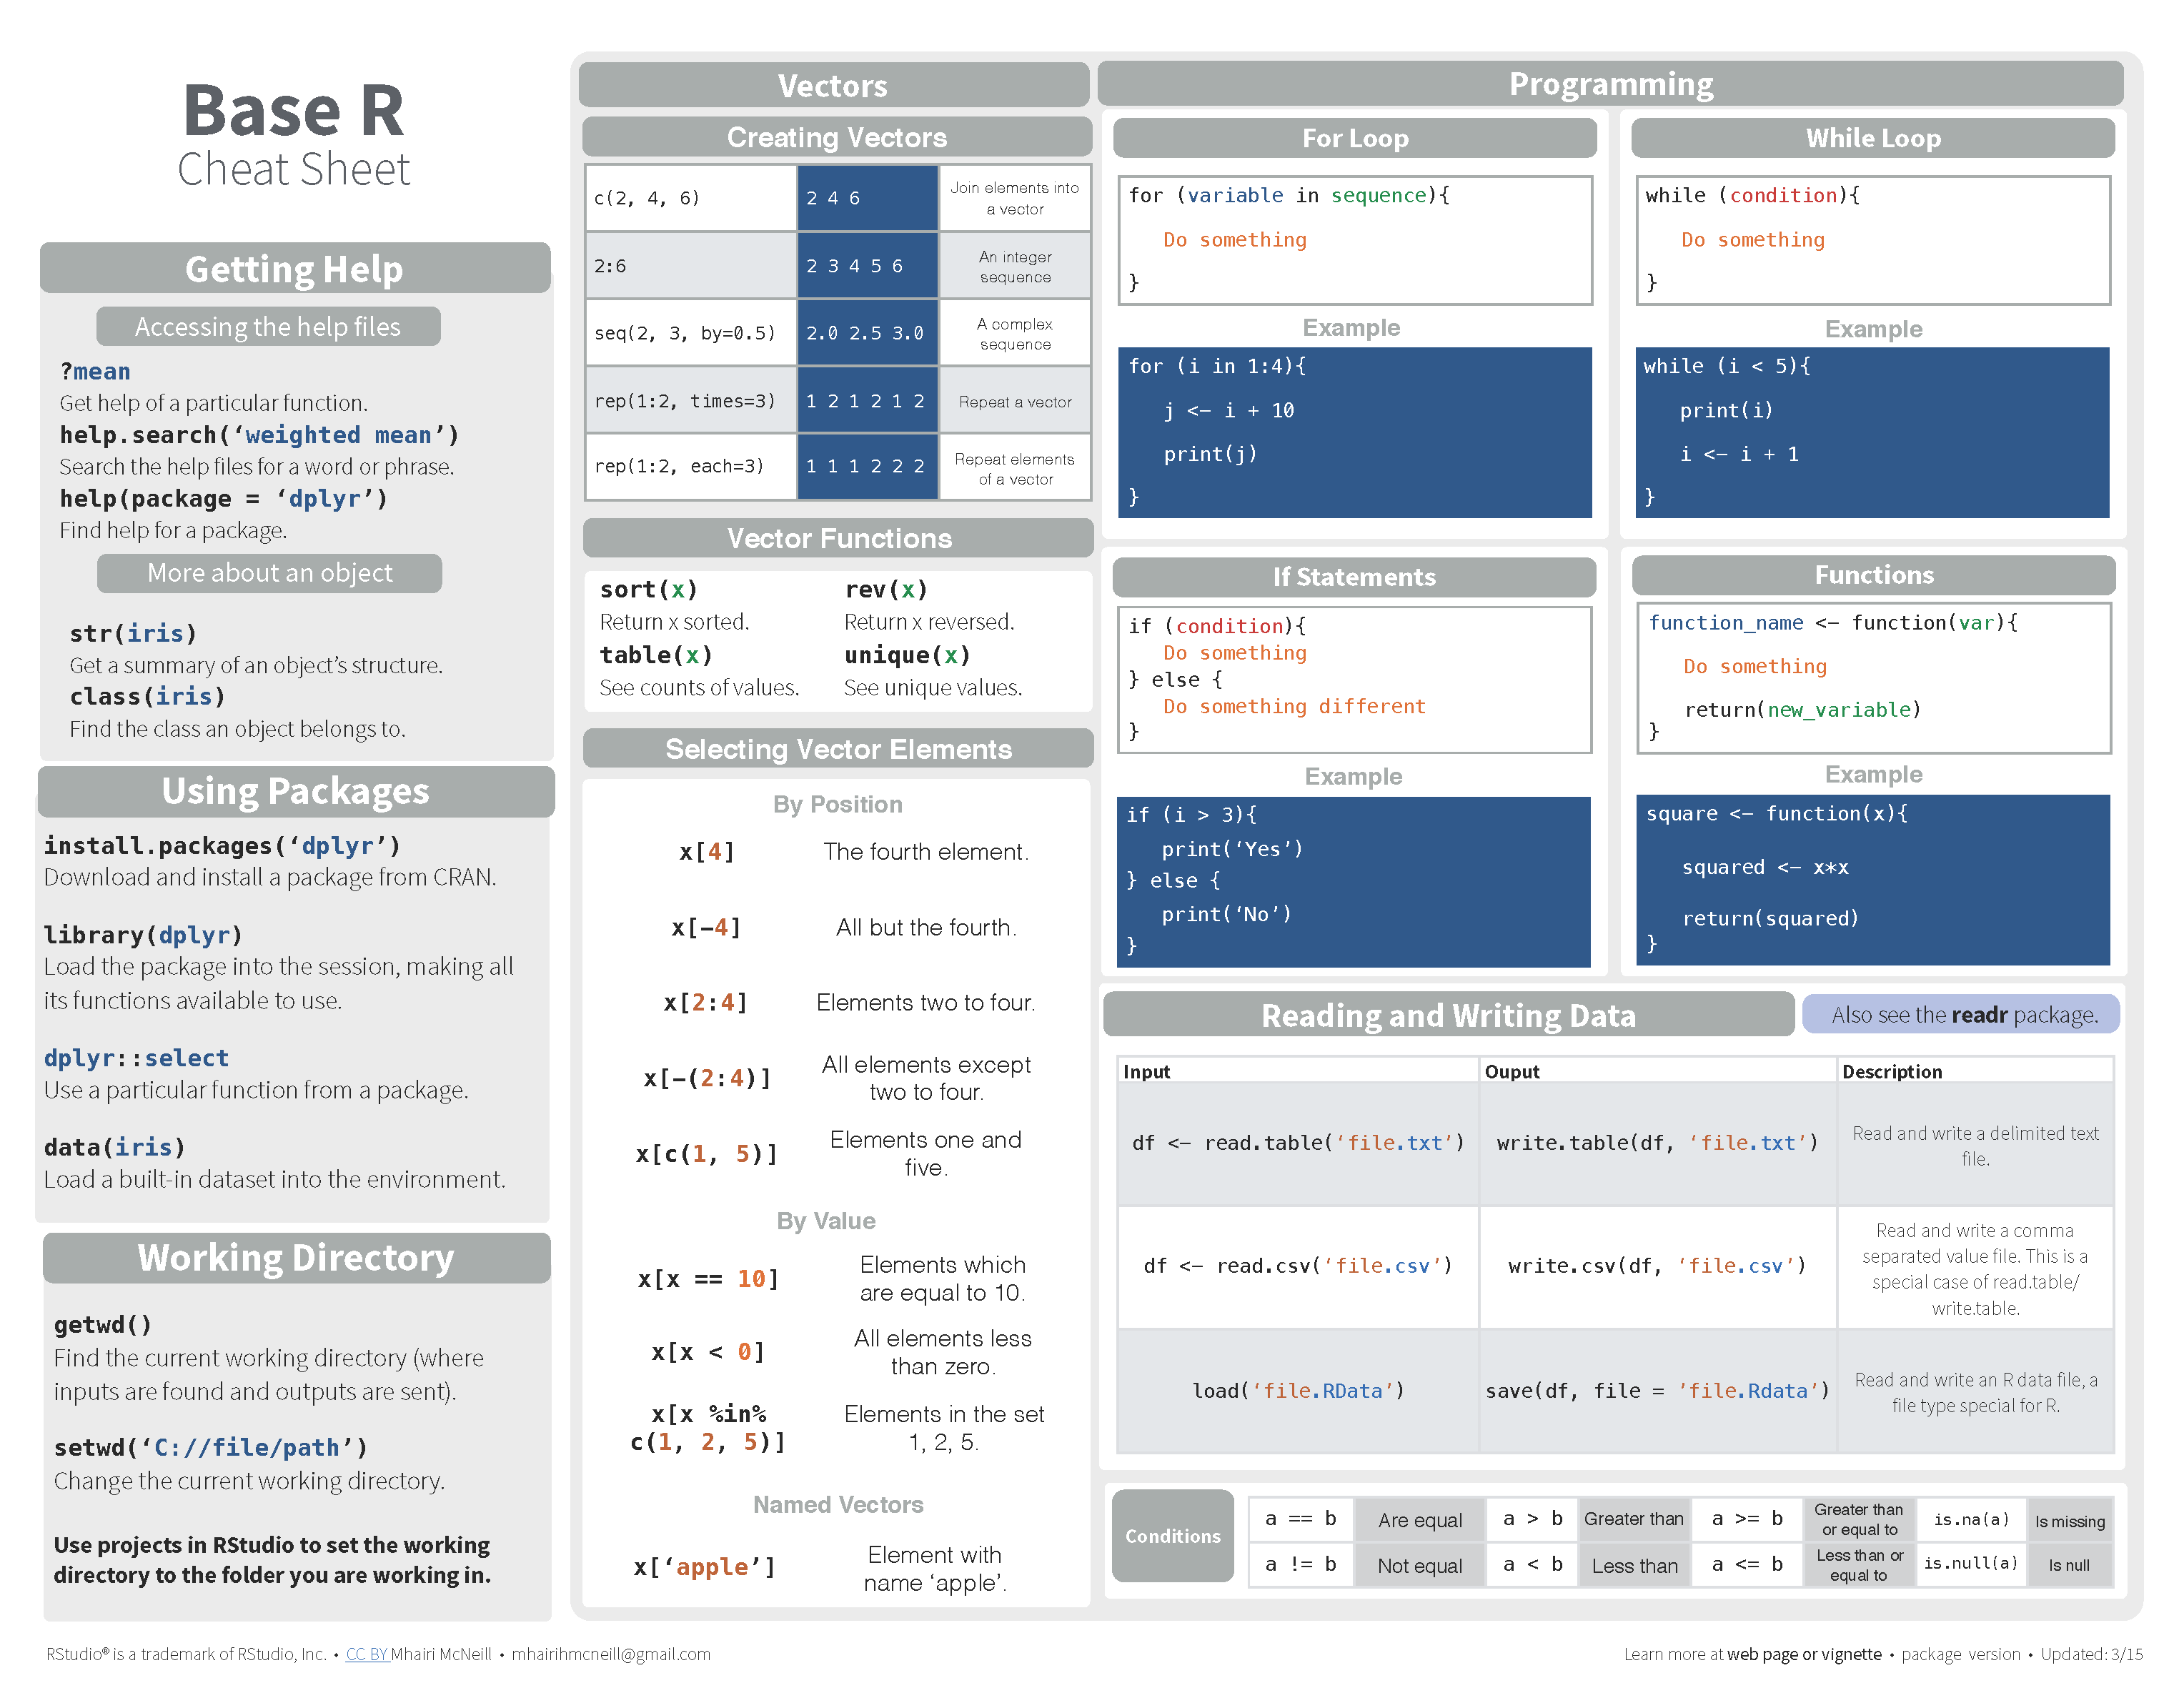
\includegraphics[width=3.64583in,height=\textheight]{images/01/base-r_1.png}
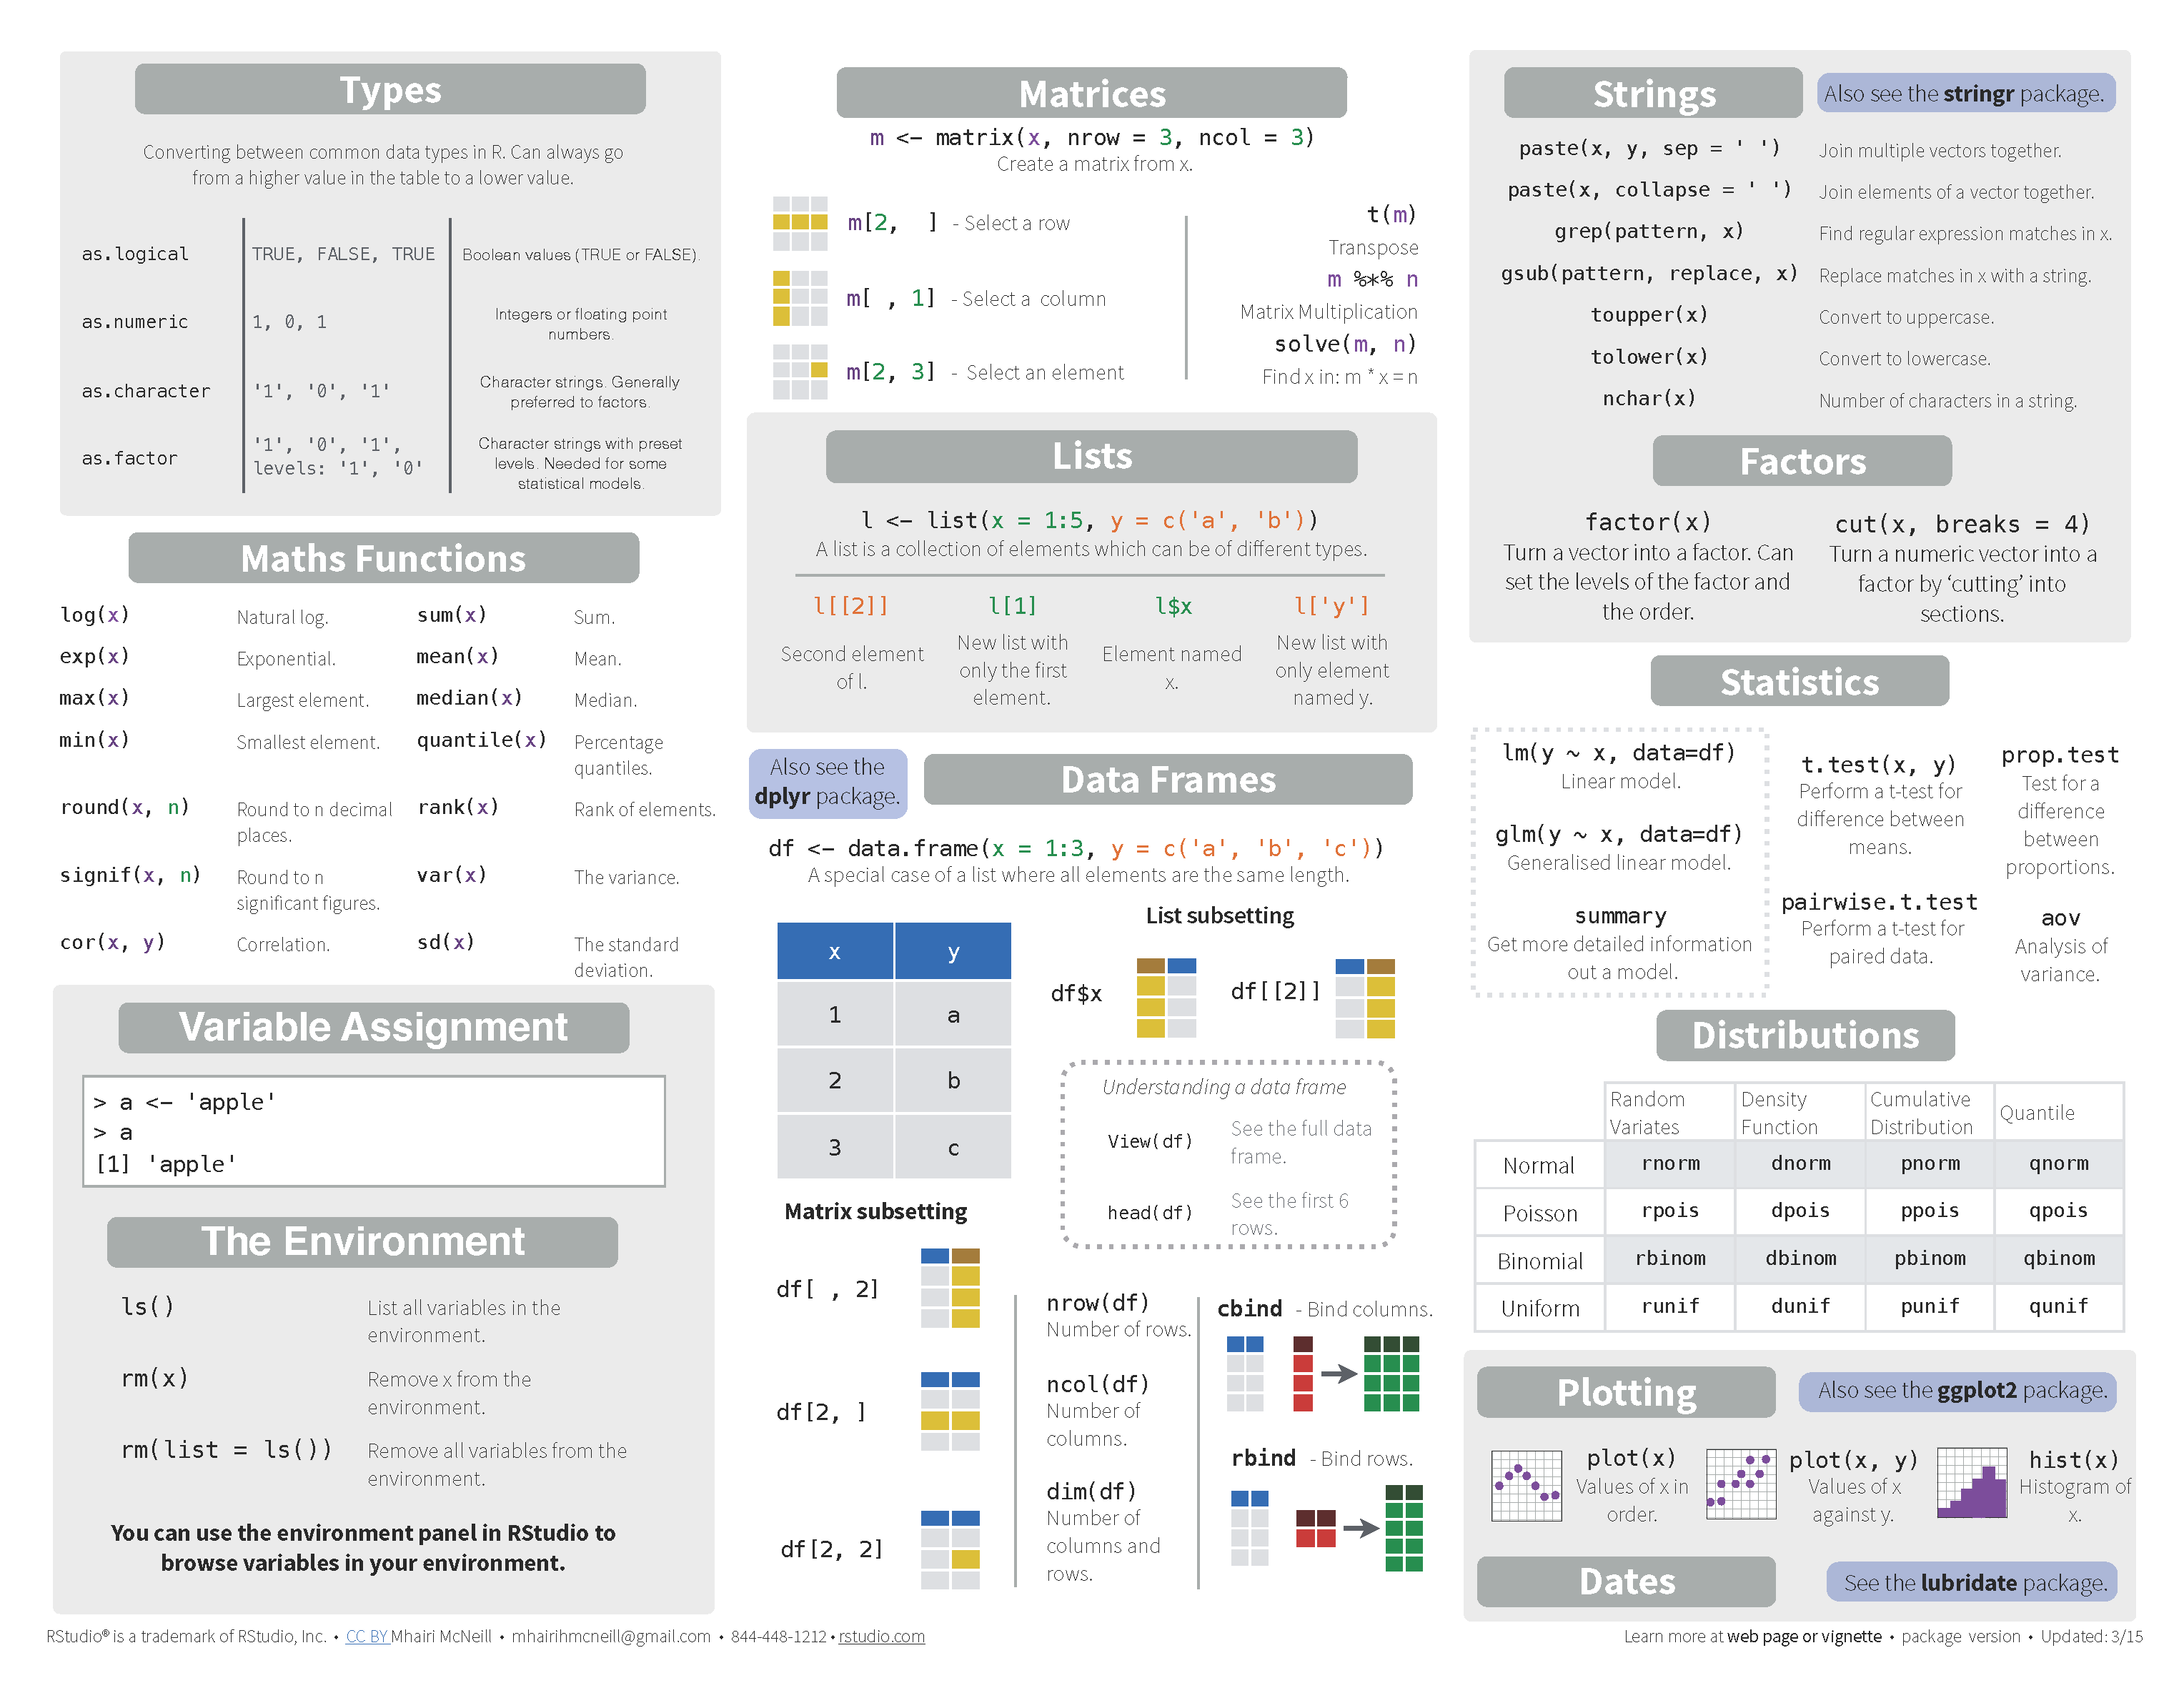
\includegraphics[width=3.64583in,height=\textheight]{images/01/base-r_2.png}

\hypertarget{r-packages-and-dataset}{%
\section{R packages and Dataset}\label{r-packages-and-dataset}}

\hypertarget{r-packages}{%
\subsection{R packages}\label{r-packages}}

\begin{itemize}
\tightlist
\item
  R 패키지는 함수들의 모음으로 다른 사람들이 만들어 놓은 함수를 가져와서 사용할 수 있음
\item
  예) \texttt{sum()} 은 \texttt{base} package에 있고 \texttt{sd()} 함수는 \texttt{stats} package에서 제공
\item
  패키지를 구할 수 있는 가장 대표적인 사이트
\item
  The Comprehensive R Archive Network (CRAN) - \url{http://cran.r-project.org/web/views/}
\item
  Bioconductor - \url{http://www.bioconductor.org/packages/release/bioc/}
\end{itemize}

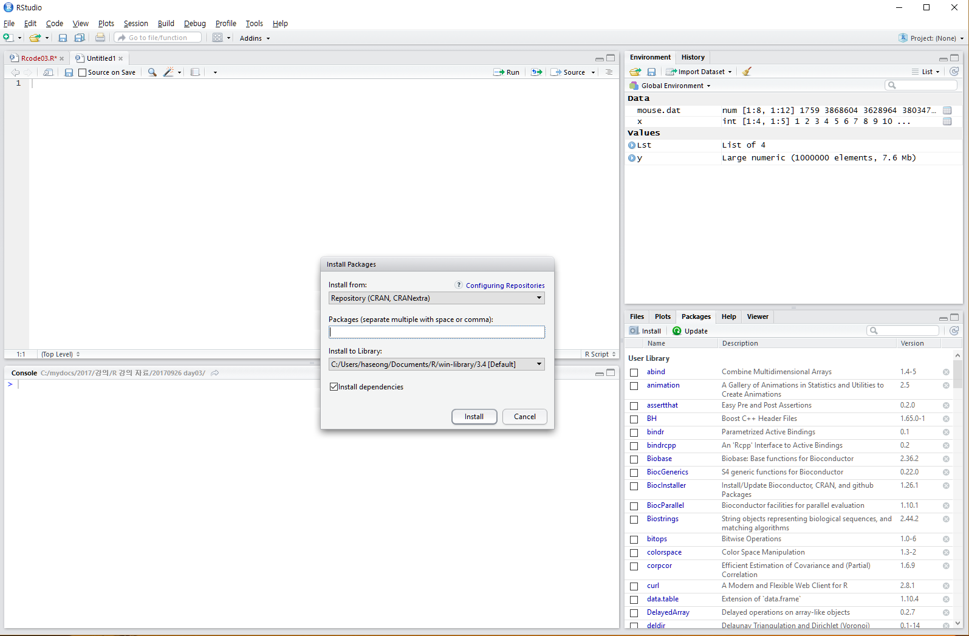
\includegraphics[width=3.64583in,height=\textheight]{images/01/01-18.png}

\begin{itemize}
\tightlist
\item
  UsingR package installation
\end{itemize}

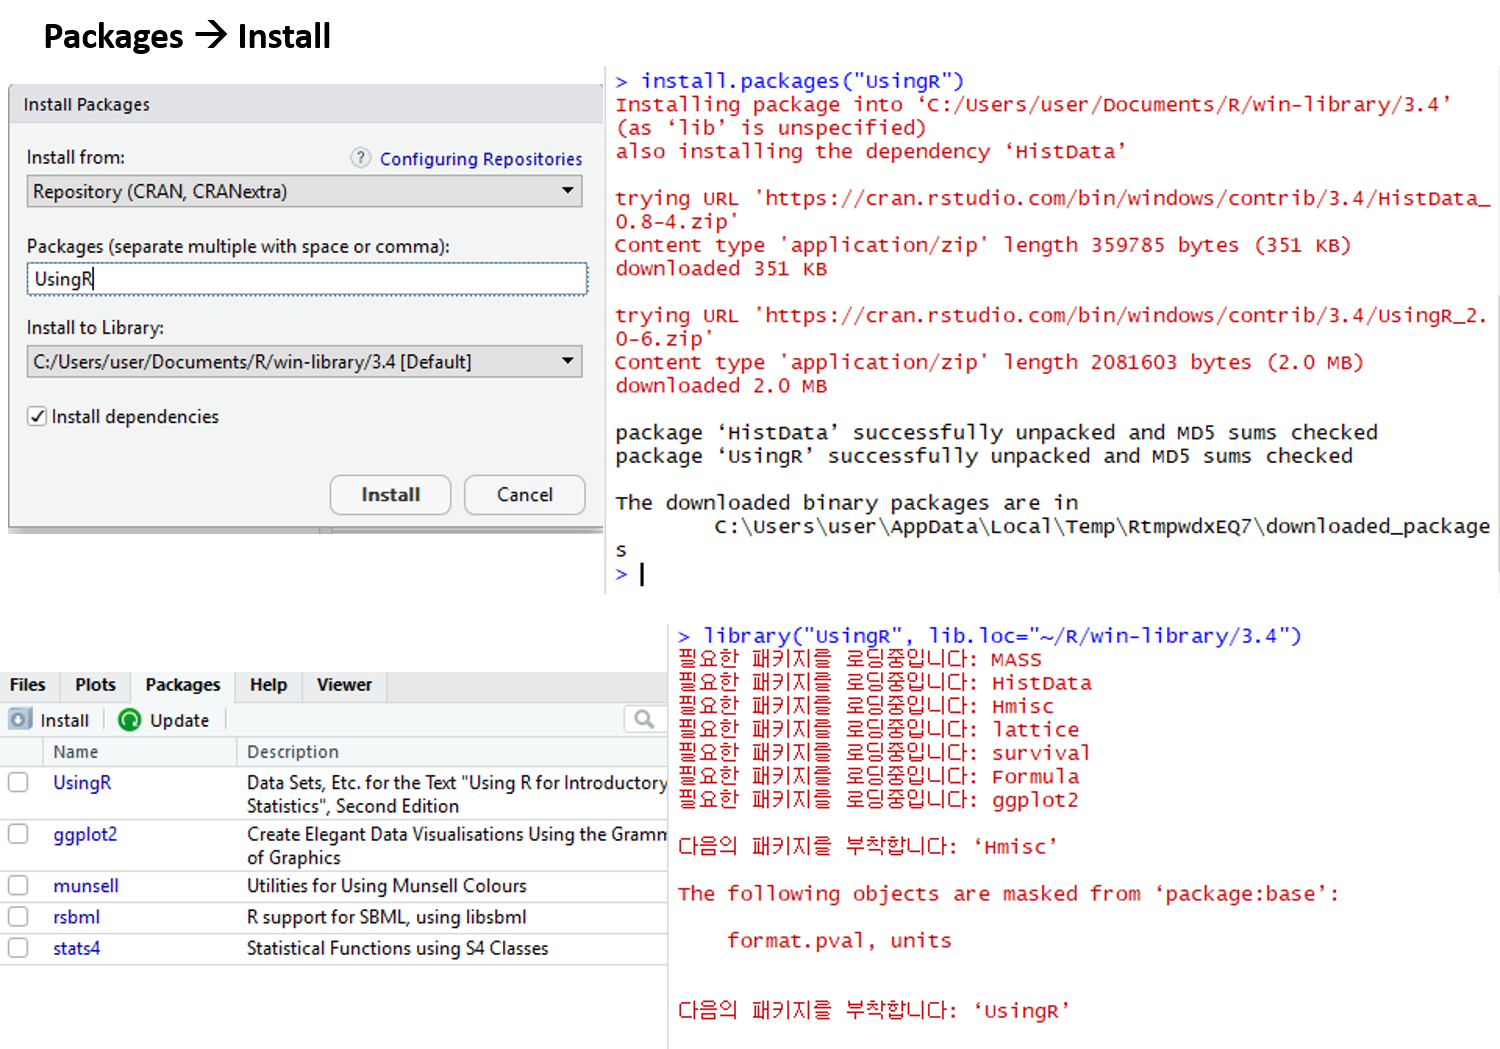
\includegraphics[width=3.64583in,height=\textheight]{images/01/01-19.png}

\begin{Shaded}
\begin{Highlighting}[]
\FunctionTok{install.packages}\NormalTok{(}\StringTok{"UsingR"}\NormalTok{)}
\end{Highlighting}
\end{Shaded}

\begin{itemize}
\tightlist
\item
  UsingR package loading
\end{itemize}

\begin{Shaded}
\begin{Highlighting}[]
\FunctionTok{library}\NormalTok{(UsingR)}
\FunctionTok{help}\NormalTok{(}\AttributeTok{package=}\StringTok{"UsingR"}\NormalTok{)}
\end{Highlighting}
\end{Shaded}

\hypertarget{data-sets}{%
\subsection{Data sets}\label{data-sets}}

\begin{itemize}
\tightlist
\item
  일반적으로 패키지 안에 관련된 데이터도 같이 저장
\item
  data() function를 이용해서 패키지 데이터를 사용자 작업공간에 복사해서 사용 가능
\end{itemize}

\begin{Shaded}
\begin{Highlighting}[]
\FunctionTok{head}\NormalTok{(rivers)}
\FunctionTok{length}\NormalTok{(rivers)}
\FunctionTok{class}\NormalTok{(rivers)}
\FunctionTok{data}\NormalTok{(rivers)}
\FunctionTok{data}\NormalTok{(}\AttributeTok{package=}\StringTok{"UsingR"}\NormalTok{)}
\FunctionTok{library}\NormalTok{(HistData)}
\FunctionTok{head}\NormalTok{(Cavendish)}
\FunctionTok{str}\NormalTok{(Cavendish)}
\FunctionTok{head}\NormalTok{(Cavendish}\SpecialCharTok{$}\NormalTok{density2)}
\end{Highlighting}
\end{Shaded}

이 저작물은 크리에이티브 커먼즈 저작자표시-비영리-변경금지 4.0 국제 라이선스에 따라 이용할 수 있습니다.

\hypertarget{tidyverse-for-data-science}{%
\chapter{Tidyverse for Data science}\label{tidyverse-for-data-science}}

tidyverse (\url{https://www.tidyverse.org/)는} 데이터 사이언스를 위한 R 기반의 독창적인 패키지들의 모음입니다. Rstudio의 핵심 전문가인 해들리위컴이 (Hadley Wickham) 중심이 되어 만들어 졌으며 기존의 툴보다 쉽고 효율적으로 데이터 분석을 수행할 수 있습니다.

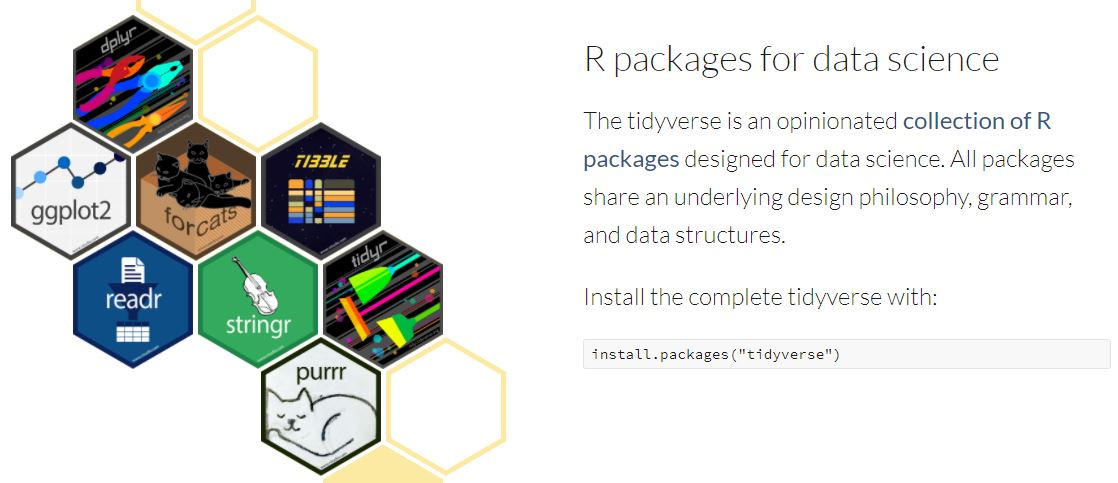
\includegraphics{images/07/tidyverse.JPG}

데이터사이언스는 넓은 범위의 개념과 방법적인 정도가 있는 것은 아닙니다. 그러나 위 tidyverse의 목적은 데이터 분석을 위한 핵심이되는 고효율의 툴을 제공하는 것이며 그 철학은 다음과 같은 그림으로 요약할 수 있습니다.

\begin{figure}
\centering
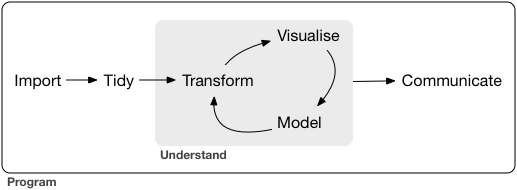
\includegraphics{images/07/data-science.png}
\caption{from \url{https://r4ds.had.co.nz/}}
\end{figure}

\hypertarget{tibble-object-type}{%
\section{Tibble object type}\label{tibble-object-type}}

R은 20년 이상된 비교적 오랜 역사를 가진 언어로서 \texttt{data.frame} 형태의 데이터 타입이 가장 많이 사용되고 있습니다. 그러나 당시에는 유용했던 기능이 시간이 흐르면서 몇몇 단점들이 드러나는 문제로 기존 코드를 그대로 유지한채 package 형태로 단점을 보완한 새로운 형태의 tibble 오브젝트 형식을 만들어 냈습니다. 대부분의 R 코드는 여전히 data.frame 형태의 데이터 타입을 사용하고 있으나 tidyverse에서는 tibble이 사용되는 것을 참고하시기 바랍니다.

\begin{Shaded}
\begin{Highlighting}[]
\FunctionTok{library}\NormalTok{(tidyverse)}

\NormalTok{tb }\OtherTok{\textless{}{-}} \FunctionTok{tibble}\NormalTok{(}
  \AttributeTok{x =} \DecValTok{1}\SpecialCharTok{:}\DecValTok{5}\NormalTok{, }
  \AttributeTok{y =} \DecValTok{1}\NormalTok{, }
  \AttributeTok{z =}\NormalTok{ x }\SpecialCharTok{\^{}} \DecValTok{2} \SpecialCharTok{+}\NormalTok{ y}
\NormalTok{)}

\FunctionTok{as\_tibble}\NormalTok{(iris)}
\FunctionTok{head}\NormalTok{(iris)}
\end{Highlighting}
\end{Shaded}

Tibble은 data.frame과 다음 몇 가지 점이 다릅니다. data.frame의 경우 타입을 변환할 때 강제로 값의 타입을 바꾸거나 내부 변수의 이름을 바꾸는 경우가 있었으나 tibble은 이를 허용하지 않습니다. 샘플들 (row) 이름을 바꿀수도 없습니다. 또한 프린팅할 때 출력물에 나오는 정보가 다르며 마지막으로 data.frame은 subset에 대한 타입이 바뀔 경우가 있었지만 tibble은 바뀌지 않습니다.

\begin{Shaded}
\begin{Highlighting}[]
\NormalTok{x }\OtherTok{\textless{}{-}} \DecValTok{1}\SpecialCharTok{:}\DecValTok{3}
\NormalTok{y }\OtherTok{\textless{}{-}} \FunctionTok{list}\NormalTok{(}\DecValTok{1}\SpecialCharTok{:}\DecValTok{5}\NormalTok{, }\DecValTok{1}\SpecialCharTok{:}\DecValTok{10}\NormalTok{, }\DecValTok{1}\SpecialCharTok{:}\DecValTok{20}\NormalTok{)}

\FunctionTok{data.frame}\NormalTok{(x, y)}
\FunctionTok{tibble}\NormalTok{(x, y)}
\end{Highlighting}
\end{Shaded}

\begin{Shaded}
\begin{Highlighting}[]
\FunctionTok{names}\NormalTok{(}\FunctionTok{data.frame}\NormalTok{(}\StringTok{\textasciigrave{}}\AttributeTok{crazy name}\StringTok{\textasciigrave{}} \OtherTok{=} \DecValTok{1}\NormalTok{))}
\FunctionTok{names}\NormalTok{(}\FunctionTok{tibble}\NormalTok{(}\StringTok{\textasciigrave{}}\AttributeTok{crazy name}\StringTok{\textasciigrave{}} \OtherTok{=} \DecValTok{1}\NormalTok{))}
\end{Highlighting}
\end{Shaded}

\begin{Shaded}
\begin{Highlighting}[]
\FunctionTok{data.frame}\NormalTok{(}\AttributeTok{x =} \DecValTok{1}\SpecialCharTok{:}\DecValTok{5}\NormalTok{, }\AttributeTok{y =}\NormalTok{ x }\SpecialCharTok{\^{}} \DecValTok{2}\NormalTok{)}
\FunctionTok{tibble}\NormalTok{(}\AttributeTok{x =} \DecValTok{1}\SpecialCharTok{:}\DecValTok{5}\NormalTok{, }\AttributeTok{y =}\NormalTok{ x }\SpecialCharTok{\^{}} \DecValTok{2}\NormalTok{)}
\end{Highlighting}
\end{Shaded}

\begin{Shaded}
\begin{Highlighting}[]
\NormalTok{df1 }\OtherTok{\textless{}{-}} \FunctionTok{data.frame}\NormalTok{(}\AttributeTok{x =} \DecValTok{1}\SpecialCharTok{:}\DecValTok{3}\NormalTok{, }\AttributeTok{y =} \DecValTok{3}\SpecialCharTok{:}\DecValTok{1}\NormalTok{)}
\FunctionTok{class}\NormalTok{(df1[, }\DecValTok{1}\SpecialCharTok{:}\DecValTok{2}\NormalTok{])}
\FunctionTok{class}\NormalTok{(df1[, }\DecValTok{1}\NormalTok{])}

\NormalTok{df2 }\OtherTok{\textless{}{-}} \FunctionTok{tibble}\NormalTok{(}\AttributeTok{x =} \DecValTok{1}\SpecialCharTok{:}\DecValTok{3}\NormalTok{, }\AttributeTok{y =} \DecValTok{3}\SpecialCharTok{:}\DecValTok{1}\NormalTok{)}
\FunctionTok{class}\NormalTok{(df2[, }\DecValTok{1}\SpecialCharTok{:}\DecValTok{2}\NormalTok{])}
\FunctionTok{class}\NormalTok{(df2[, }\DecValTok{1}\NormalTok{])}
\FunctionTok{class}\NormalTok{(df2}\SpecialCharTok{$}\NormalTok{x)}
\end{Highlighting}
\end{Shaded}

\hypertarget{tidy-data-structure}{%
\section{Tidy data structure}\label{tidy-data-structure}}

데이터의 변수와 값을 구분하는 일은 적절한 데이터 분석을 위해 필수적인 과정입니다. 특히 복잡하고 사이즈가 큰 데이터일 경우는 더욱 중요할 수 있으나 경험에 의존해서 구분을 하는 것이 대부분 입니다. Tidy data는 이러한 변수와 값의 명확한 구분과 활용을 위한 데이터 구조중 하나 입니다 (Hadley Wickham. Tidy data. \emph{The Journal of Statistical Software}, vol.~59, 2014).

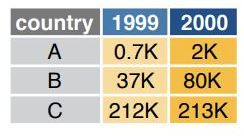
\includegraphics{images/07/notidy.JPG}

tidy data는 다음과 같은 특징이 있습니다.

\begin{itemize}
\tightlist
\item
  각 변수는 해당하는 유일한 하나의 column을 가짐
\item
  각 샘플은 해당하는 유일한 하나의 row를 가짐
\item
  각 관측값은 해당하는 유일한 하나의 cell을 가짐
\end{itemize}

\begin{figure}
\centering
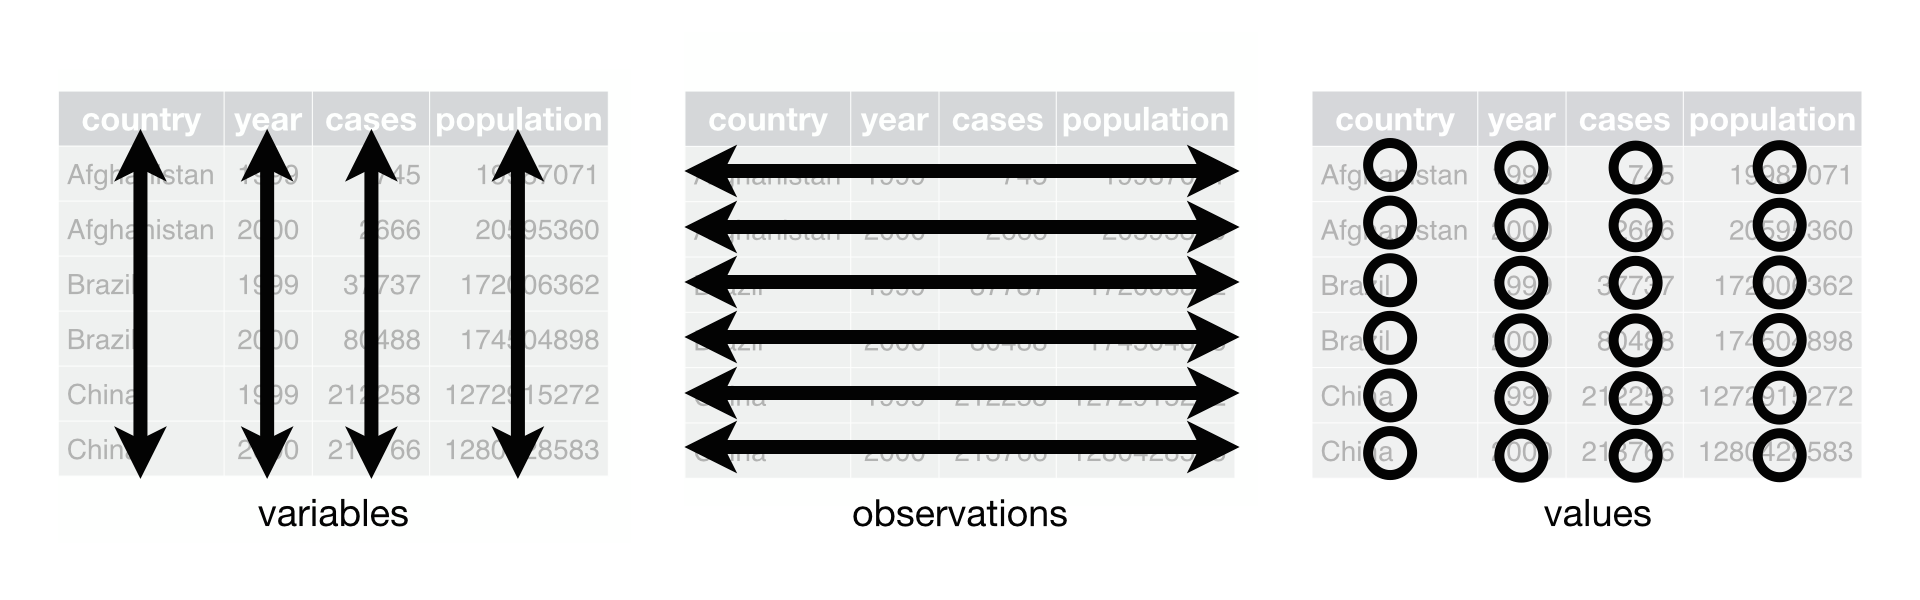
\includegraphics[width=4.6875in,height=\textheight]{images/07/tidy-1.png}
\caption{from \url{https://r4ds.had.co.nz/}}
\end{figure}

Tidy 데이터는 Long형 데이터로 알려져 있기도 합니다. 참고로 Wide형 데이터의 경우 샘플 데이터가 늘어날수록 row에 쌓이고 새로운 변수는 column에 쌓이는 방식으로 데이터가 확장되는 형태 입니다. 엑셀에서 볼 수 있는 일반적인 형식으로 다음 그림과 같습니다.

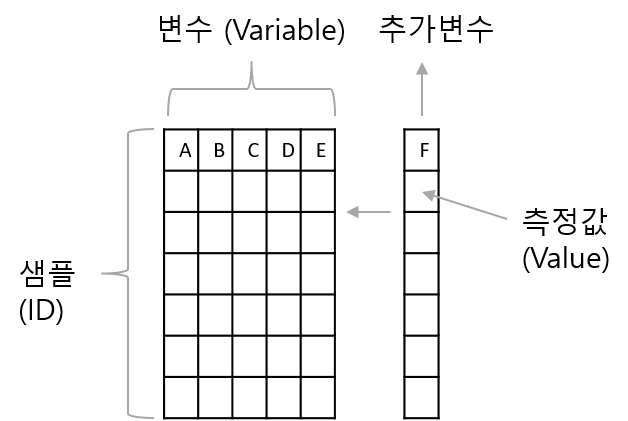
\includegraphics[width=3.125in,height=\textheight]{images/07/05.png}

Long형 데이터의 경우 ID, variable, value 세가지 변수만 기억하면 되겠습니다. 위 wide형 데이터 경우를 보면 ID, variable, 그리고 value 이 세가지 요인이 주요 구성 요소임을 알 수 있습니다. Long형으로 변환할 경우 샘플을 참조할 수 있는 어떤 변수 (variable)도 ID가 될 수 있으며 2개 이상의 변수가 ID로 지정될 수 있습니다. 참고로 ID를 지정할 경우 해당 ID는 가능하면 중복되지 않는 값들을 갖는 변수를 사용해야 식별자로서 기능을 적절히 수행할 수 있습니다. Long형을 사용할 경우 데이터의 변수가 늘어나도 행의 수만 늘어나므로 코딩의 일관성과 변수들의 그룹을 만들어서 분석하는 등의 장점이 있습니다. 아래는 새로운 변수 F가 추가될 때 long 형 데이터에 데이터가 추가되는 경우를 나타낸 그림 입니다.

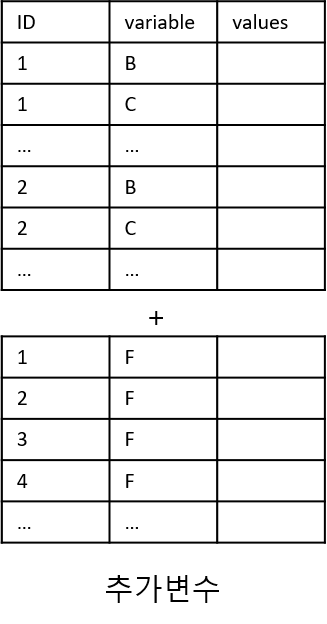
\includegraphics[width=\textwidth,height=3.64583in]{images/07/06.png}

\hypertarget{pivoting}{%
\section{Pivoting}\label{pivoting}}

일반적으로 얻어지는 데이터의 형태는 wide형이며 이를 Long형으로 변환하기 위해서는 \texttt{tidyverse} 패키지에 속한 \texttt{tidyr} 패키지의 \texttt{pivot\_longer}와 \texttt{pivot\_wider}를 사용합니다. 또한 \texttt{reshape2} 패키지의 \texttt{melt}함수와 그 반대의 경우 \texttt{dcast} 함수를 사용할 수도 있습니다. 본 강의에서는 \texttt{tidyr} 패키지를 사용합니다. wide형 데이터를 long형으로 변환하거나 long형을 wide형으로 변환하는 작업을 pivoting 이라고 합니다.

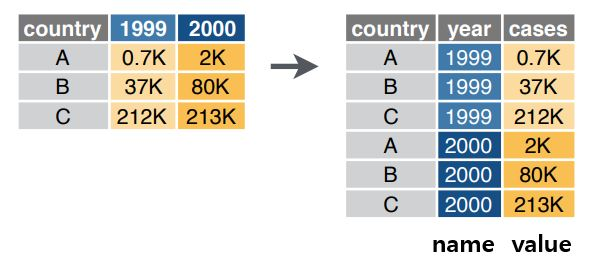
\includegraphics[width=4.6875in,height=\textheight]{images/07/wide2long.JPG}

\texttt{airquality} 데이터는 전형적인 wide형 데이터로 특정 날짜에 네 개의 변수에 해당하는 값들을 측정했습니다. 이 데이터를 long형으로 바꿀 경우 ID를 날짜로 하면 데이터들을 식별 할 수 있습니다. 그런데 날짜는 변수가 Month와 Day두 개로 나누어져 있으므로 다음과 같이 두 변수를 식별 변수로 (ID로) 사용 합니다. 확인을 위해 상위 5개의 데이터만 가지고 형 변환을 진행해 보겠습니다.

\begin{Shaded}
\begin{Highlighting}[]
\NormalTok{airquality}

\NormalTok{myair }\OtherTok{\textless{}{-}}\NormalTok{ airquality[}\DecValTok{1}\SpecialCharTok{:}\DecValTok{5}\NormalTok{,]}
\NormalTok{myair\_long }\OtherTok{\textless{}{-}} \FunctionTok{pivot\_longer}\NormalTok{(myair, }\FunctionTok{c}\NormalTok{(}\StringTok{"Ozone"}\NormalTok{, }\StringTok{"Solar.R"}\NormalTok{, }\StringTok{"Wind"}\NormalTok{, }\StringTok{"Temp"}\NormalTok{))}
\NormalTok{myair\_long }
\NormalTok{myair\_long2 }\OtherTok{\textless{}{-}} \FunctionTok{pivot\_longer}\NormalTok{(myair, }\FunctionTok{c}\NormalTok{(Ozone, Solar.R, Wind, Temp))}
\NormalTok{myair\_long2 }
\NormalTok{myair\_long3 }\OtherTok{\textless{}{-}} \FunctionTok{pivot\_longer}\NormalTok{(myair, }\SpecialCharTok{!}\FunctionTok{c}\NormalTok{(Month, Day))}
\NormalTok{myair\_long3}
\end{Highlighting}
\end{Shaded}

생성되는 long형 데이터의 변수 이름인 name과 value는 다음 파라메터를 지정하여 바꿀 수 있습니다.

\begin{Shaded}
\begin{Highlighting}[]
\NormalTok{myair\_long }\OtherTok{\textless{}{-}} \FunctionTok{pivot\_longer}\NormalTok{(myair, }
                          \FunctionTok{c}\NormalTok{(Ozone, Solar.R, Wind, Temp), }
                          \AttributeTok{names\_to =} \StringTok{"Type"}\NormalTok{, }
                          \AttributeTok{values\_to =} \StringTok{"Observation"}\NormalTok{)}
\NormalTok{myair\_long }
\end{Highlighting}
\end{Shaded}

long형 데이터를 wide형 데이터로 변환 할 수도 있습니다.

\begin{Shaded}
\begin{Highlighting}[]
\FunctionTok{pivot\_wider}\NormalTok{(myair\_long, }\AttributeTok{names\_from =}\NormalTok{ Type, }\AttributeTok{values\_from =}\NormalTok{ Observation)}
\end{Highlighting}
\end{Shaded}

\hypertarget{ex7.3.1}{%
\subsection{Exercise}\label{ex7.3.1}}

\begin{enumerate}
\def\labelenumi{\arabic{enumi})}
\tightlist
\item
  다음 데이터가 long형인지 wide형인지 판단하시오\\
\item
  long형이면 wide형으로 wide형이면 long형으로 변환하시오
\end{enumerate}

\begin{Shaded}
\begin{Highlighting}[]
\NormalTok{stocks }\OtherTok{\textless{}{-}} \FunctionTok{tibble}\NormalTok{(}
  \AttributeTok{year   =} \FunctionTok{c}\NormalTok{(}\DecValTok{2015}\NormalTok{, }\DecValTok{2015}\NormalTok{, }\DecValTok{2016}\NormalTok{, }\DecValTok{2016}\NormalTok{),}
  \AttributeTok{month  =} \FunctionTok{c}\NormalTok{(   }\DecValTok{1}\NormalTok{,    }\DecValTok{2}\NormalTok{,     }\DecValTok{1}\NormalTok{,    }\DecValTok{2}\NormalTok{),}
  \AttributeTok{profit =} \FunctionTok{c}\NormalTok{(}\FloatTok{1.88}\NormalTok{, }\FloatTok{0.59}\NormalTok{, }\FloatTok{0.92}\NormalTok{, }\FloatTok{0.17}\NormalTok{)}
\NormalTok{)}
\end{Highlighting}
\end{Shaded}

\texttt{ggplot}을 이용한 그래프 작성에는 위와 같은 long형 데이터가 주로 사용됩니다. R을 이용한 데이터 가시화는 \texttt{dplyr} 패키지로 wide형 데이터를 편집하고 \texttt{pivot\_longer} 함수로 long형 데이터로 변환 후 \texttt{ggplot}을 이용하는 방식으로 수행합니다. 두 데이터 포멧에 대한 좀 더 구체적인 내용은 다음 링크를 참고하시기 바랍니다. \url{https://www.theanalysisfactor.com/wide-and-long-data/}

\hypertarget{separating-and-uniting}{%
\section{Separating and uniting}\label{separating-and-uniting}}

데이터를 분석할 때 하나의 컬럼에 두 개 이상의 변수값이 저장되어 있거나 두 개의 변수를 하나의 컬럼으로 합해야 하는 경우가 종종 있습니다. 전자의 경우 \texttt{separate()} 함수를 사용해서 두 변수(컬럼)으로 나누어 줄 수 있으며 후자의 경우 \texttt{unite()} 함수를 사용하여 두 변수를 하나의 값으로 병합할 수 있습니다. 다음은 \texttt{airquality}데이터에서 Month와 Day 변수를 하나의 컬럼으로 병합하여 Date라는 변수로 만들어 주는 경우의 예 입니다.

\begin{Shaded}
\begin{Highlighting}[]
\NormalTok{newairquality }\OtherTok{\textless{}{-}} \FunctionTok{unite}\NormalTok{(airquality, Date, Month, Day, }\AttributeTok{sep=}\StringTok{"."}\NormalTok{)}
\NormalTok{newairquality}
\end{Highlighting}
\end{Shaded}

\texttt{separate()}함수를 사용하면 다음과 같이 해당 변수의 값을 나누어 다시 두 개의 변수(컬럼)으로 나누어 줄 수 있습니다.

\begin{Shaded}
\begin{Highlighting}[]
\FunctionTok{separate}\NormalTok{(newairquality, }\AttributeTok{col=}\NormalTok{Date, }\AttributeTok{into =} \FunctionTok{c}\NormalTok{(}\StringTok{"Month"}\NormalTok{, }\StringTok{"Day"}\NormalTok{), }\AttributeTok{sep =} \StringTok{"}\SpecialCharTok{\textbackslash{}\textbackslash{}}\StringTok{."}\NormalTok{)}
\end{Highlighting}
\end{Shaded}

\hypertarget{dplyr-and-pipe-operator}{%
\section{dplyr and pipe operator}\label{dplyr-and-pipe-operator}}

\texttt{dplyr} (\url{https://dplyr.tidyverse.org/}) 은 \texttt{ggplot2}을 개발한 해들리위컴이 (Hadley Wickham) 중심이 되어 만들어 졌으며 \texttt{ggplot2}와 함께 \texttt{tidyverse}의 (\url{https://www.tidyverse.org/}) 핵심 패키지 입니다. \texttt{dplyr}은 데이터를 다루는 크기나 분석의 속도, 편의성을 향상시켜 새롭게 만들어놓은 패키지 입니다. 기존 \texttt{apply}와 같은 행렬 연산 기능과 \texttt{subset}, \texttt{split}, \texttt{group} 와 같은 행렬 편집 기능을 더하여 만들어진 도구라고 할 수 있습니다.

\texttt{dplyr}의 전신이라 할 수 있는 \texttt{plyr} 패키지는 다음과 같이 설명이 되어 있습니다. \emph{A set of tools for a common set of problems: you need to split up a big data structure into homogeneous pieces, apply a function to each piece and then combine all the results back together.} 즉 split-apply-combine 세 가지 동작을 쉽게 할 수 있도록 만들어 놓은 툴 입니다. R이 다른 언어에 비해 데이터 분석에서 주목을 받는 이유로 \texttt{split}, \texttt{apply} 등의 행렬 연산 함수가 발달한 것을 내세우는데 \texttt{dplyr}은 이들을 보다 더 편리하게 사용할 수 있도록 만들어 놓은 것 입니다.

\texttt{dplyr}의 사용을 위해서는 여러 명령을 연속적으로 수행하도록 해주는 \texttt{\%\textgreater{}\%} 파이프 오퍼레이터의 이해가 필요합니다. 파이프 오퍼레이터의 작동법은 간단히 \texttt{\%\textgreater{}\%}의 왼쪽 코드의 결과를 출력으로 받아 오른쪽 코드의 입력 (첫번째 파라미터의 값)으로 받아들이는 작동을 합니다 (\textbf{단축키: Shift+Ctrl+m}). 다음 예에서 보면 \texttt{sin(pi)} 와 같은 함수의 일반적인 사용법 대신 \texttt{pi\ \%\textgreater{}\%\ sin} 처럼 사용해도 똑같은 결과를 보여줍니다. \texttt{cos(sin(pi))}와 같이 여러 합수를 중첩하여 사용할 경우와 비교해서 코드의 가독성이나 효율 측면에서 크게 향상된 방법을 제공해 줍니다.

\begin{Shaded}
\begin{Highlighting}[]
\FunctionTok{library}\NormalTok{(dplyr)}

\NormalTok{pi }\SpecialCharTok{\%\textgreater{}\%}\NormalTok{ sin}
\FunctionTok{sin}\NormalTok{(pi)}
\NormalTok{pi }\SpecialCharTok{\%\textgreater{}\%}\NormalTok{ sin }\SpecialCharTok{\%\textgreater{}\%}\NormalTok{ cos}
\FunctionTok{cos}\NormalTok{(}\FunctionTok{sin}\NormalTok{(pi))}
\end{Highlighting}
\end{Shaded}

특히 \texttt{\%\textgreater{}\%}는 이후 설명할 \texttt{dplyr}의 \texttt{group\_by}, \texttt{split}, \texttt{filter}, \texttt{summary} 등의 행렬 편집/연산 함수를 빈번히 다양한 조합으로 쓰게되는 상황에서 더 큰 효과를 발휘할 수 있습니다.

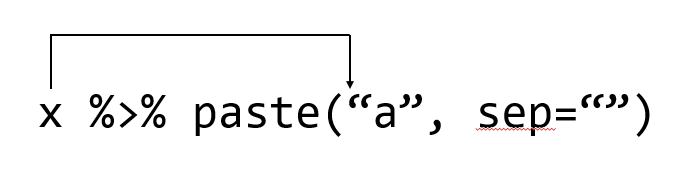
\includegraphics{images/07/02.PNG}

pipe operator의 왼쪽 구문의 결과가 오른쪽 구문의 첫 번째 파라미터의 입력 값으로 처리된다고 말씀 드렸습니다. 즉, 함수에서 사용되는 파라미터가 여러개일 경우가 있으므로 기본적으로 \texttt{\%\textgreater{}\%} 의 왼쪽 구문의 출력 값은 오른쪽 구문 (함수)의 첫 번째 인자의 입력값으로 들어가는 것 입니다. 이는 다음 예들을 통해서 명확히 알 수 있습니다. 먼저 \texttt{paste}함수는 그 파라미터로 \texttt{,}로 구분되는 여러개의 입력 값을 가질 수 있습니다. 따라서 다음 코드는 \texttt{x}가 \texttt{paste}의 첫 번째 파라미터로 들어가게 되어 \texttt{"1a",\ "2a",\ "3a",\ "4a",\ "5a"}로 a 앞에 x 값들이 붙어서 출력된 것을 알 수 있습니다.

\begin{Shaded}
\begin{Highlighting}[]
\NormalTok{x }\OtherTok{\textless{}{-}} \DecValTok{1}\SpecialCharTok{:}\DecValTok{5}
\NormalTok{x }\SpecialCharTok{\%\textgreater{}\%} \FunctionTok{paste}\NormalTok{(}\StringTok{"a"}\NormalTok{, }\AttributeTok{sep=}\StringTok{""}\NormalTok{)}
\end{Highlighting}
\end{Shaded}

특정 데이터셋의 컬럼별 평균을 구하고 각 평균의 합을 구할 경우를 생각해 봅시다. R에서는 \texttt{colMeans}라는 특별한 함수를 제공하여 컬럼별로 평균을 계산해 줍니다. 그 후 sum 함수를 사용하여 최종 원하는 값을 얻을 수 있습니다. 이러한 코드를 \texttt{\%\textgreater{}\%} 오퍼레이터를 사용한 경우의 코드와 비교해 볼 수 있습니다.

\begin{Shaded}
\begin{Highlighting}[]
\NormalTok{x }\OtherTok{\textless{}{-}} \FunctionTok{data.frame}\NormalTok{(}\AttributeTok{x=}\FunctionTok{c}\NormalTok{(}\DecValTok{1}\SpecialCharTok{:}\DecValTok{100}\NormalTok{), }\AttributeTok{y=}\FunctionTok{c}\NormalTok{(}\DecValTok{201}\SpecialCharTok{:}\DecValTok{300}\NormalTok{))}
\FunctionTok{sum}\NormalTok{(}\FunctionTok{colMeans}\NormalTok{(x))}

\NormalTok{x }\OtherTok{\textless{}{-}} \FunctionTok{data.frame}\NormalTok{(}\AttributeTok{x=}\FunctionTok{c}\NormalTok{(}\DecValTok{1}\SpecialCharTok{:}\DecValTok{100}\NormalTok{), }\AttributeTok{y=}\FunctionTok{c}\NormalTok{(}\DecValTok{201}\SpecialCharTok{:}\DecValTok{300}\NormalTok{))}
\NormalTok{x }\SpecialCharTok{\%\textgreater{}\%}\NormalTok{ colMeans }\SpecialCharTok{\%\textgreater{}\%}\NormalTok{ sum}
\end{Highlighting}
\end{Shaded}

그럼 만약 두 번째 파라미터에 입력으로 왼쪽 구문의 출력을 받아들이고 싶을 경우는 place holer \texttt{.} 을 사용하면 되겠습니다. \texttt{round} 함수는 두 개의 파라미터를 설정할 있 이으며 digits 라는 두 번째 파라미터에 값을 pipe operator로 넘겨주고 싶을 경우 아래와 같이 표현할 수 있습니다.

\begin{Shaded}
\begin{Highlighting}[]
\DecValTok{6} \SpecialCharTok{\%\textgreater{}\%} \FunctionTok{round}\NormalTok{(pi, }\AttributeTok{digits=}\NormalTok{.)}
\FunctionTok{round}\NormalTok{(pi, }\AttributeTok{digits=}\DecValTok{6}\NormalTok{)}
\end{Highlighting}
\end{Shaded}

\hypertarget{ex7.5.1}{%
\subsection{Exercise}\label{ex7.5.1}}

\begin{enumerate}
\def\labelenumi{\arabic{enumi})}
\tightlist
\item
  pipe operator를 사용해서 \texttt{airquality}데이터를 long형으로 전환하는 코드를 작성하시오 (단 col 파라메터에는 Ozone, Solar.R, Wind, Temp 변수를 넣음)\\
\item
  pipe operator를 사용해서 \texttt{airquality}데이터의 Month와 Day 변수(컬럼)을 Date 변수로 병합하는 코드를 작성하시오
\end{enumerate}

\hypertarget{dplyr---important-functions}{%
\section{dplyr - Important functions}\label{dplyr---important-functions}}

이제 \texttt{dplyr} 패키지에서 제공하는 함수를 사용해 보겠습니다. \texttt{dplyr}을 구성하는 중요한 함수는 다음과 같습니다.

\begin{itemize}
\tightlist
\item
  \texttt{filter()} - 샘플 (rows) 선택
\item
  \texttt{arrange()} - 샘플들의 정렬 순서 변경
\item
  \texttt{select()} - 변수 (columns) 선택
\item
  \texttt{mutate()} - 새로운 변수 만들기
\item
  \texttt{summarise()} - 대표값 만들기
\item
  \texttt{group\_by()} - 그룹별로 계산 수행
\item
  \texttt{join()} - 두 tibble 또는 data.frame을 병합할 때 사용
\end{itemize}

이 함수들은 \texttt{\%\textgreater{}\%}와 함께 쓰이면서 강력한 성능을 발휘합니다. \texttt{summarise} 함수는 특정 값들의 통계 값을 계산해 주는 함수이며 그 외 함수들은 행렬 편집을 위한 함수들로 보시면 되겠습니다. 간단한 예제를 수행하면서 각각의 기능을 살펴보고 왜 \texttt{dplyr}이 널리 사용되고 그 장점이 무엇인지 파악해 보도록 하겠습니다.

\texttt{iris} 데이터는 세 종류의 iris 품종에 대한 꽃잎과 꽃받침의 length와 with를 측정해 놓은 데이터 입니다. \texttt{head}와 \texttt{str} 명령어를 \texttt{\%\textgreater{}\%}를 이용해서 데이터를 살펴 봅니다.

\begin{Shaded}
\begin{Highlighting}[]
\FunctionTok{library}\NormalTok{(tidyverse)}

\NormalTok{iris }\SpecialCharTok{\%\textgreater{}\%} \FunctionTok{head}\NormalTok{(}\DecValTok{10}\NormalTok{)}
\NormalTok{iris }\SpecialCharTok{\%\textgreater{}\%}\NormalTok{ str}
\end{Highlighting}
\end{Shaded}

\hypertarget{filter}{%
\subsection{filter}\label{filter}}

먼저 아래와 같이 \texttt{filter} 함수를 사용해서 원하는 조건의 데이터 (샘플)을 골라낼 수 있습니다.

\begin{Shaded}
\begin{Highlighting}[]
\FunctionTok{library}\NormalTok{(dplyr)}

\FunctionTok{head}\NormalTok{(iris)}
\NormalTok{iris }\SpecialCharTok{\%\textgreater{}\%} \FunctionTok{filter}\NormalTok{(Species}\SpecialCharTok{==}\StringTok{"setosa"}\NormalTok{)}
\NormalTok{iris }\SpecialCharTok{\%\textgreater{}\%} \FunctionTok{filter}\NormalTok{(Species}\SpecialCharTok{==}\StringTok{"setosa"} \SpecialCharTok{|}\NormalTok{ Species}\SpecialCharTok{==}\StringTok{"versicolor"}\NormalTok{)}
\NormalTok{iris }\SpecialCharTok{\%\textgreater{}\%} \FunctionTok{filter}\NormalTok{(Species}\SpecialCharTok{==}\StringTok{"setosa"} \SpecialCharTok{\&}\NormalTok{ Species}\SpecialCharTok{==}\StringTok{"versicolor"}\NormalTok{)}
\NormalTok{iris }\SpecialCharTok{\%\textgreater{}\%} 
  \FunctionTok{filter}\NormalTok{(Species}\SpecialCharTok{==}\StringTok{"setosa"} \SpecialCharTok{|}\NormalTok{ Species}\SpecialCharTok{==}\StringTok{"versicolor"}\NormalTok{) }\SpecialCharTok{\%\textgreater{}\%} 
\NormalTok{  dim}
\end{Highlighting}
\end{Shaded}

\texttt{filter}의 \texttt{,}로 구분되는 매개변수는 \texttt{and} 로직으로 묶인 조건입니다. 지난 강좌에서 보셨듯 R에서 \texttt{and}는 \texttt{\&}, \texttt{or}는 \texttt{\textbar{}}, 그리고 not은 \texttt{!} 으로 사용하면 되며 \texttt{filter}에서 \texttt{,}로 구분된 조건은 \texttt{and}와 같다고 보시면 되겠습니다.

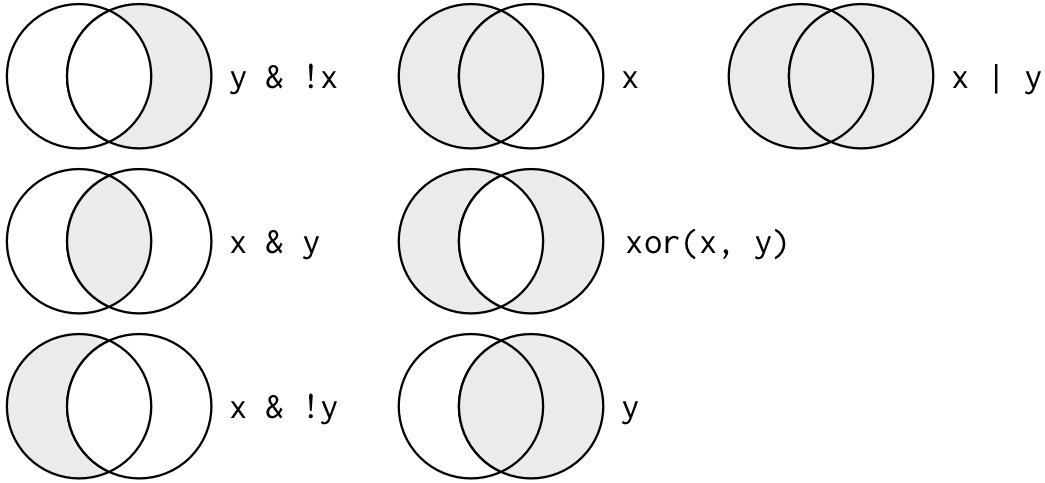
\includegraphics{images/07/03.png}

Image from (\url{https://r4ds.had.co.nz/})

\hypertarget{arrange}{%
\subsection{arrange}\label{arrange}}

\texttt{arrange()}는 지정된 변수를 기준으로 값의 크기순서로 샘플들의 배열 순서 즉, row의 순서를 바꾸는 기능을 수행합니다. 기본으로 크기가 커지는 순서로 정렬이 진행되며 작아지는 순서를 원할 경우 \texttt{desc} 함수를 사용할 수 있습니다.

\begin{Shaded}
\begin{Highlighting}[]
\NormalTok{iris }\SpecialCharTok{\%\textgreater{}\%} \FunctionTok{arrange}\NormalTok{(Sepal.Length)}
\NormalTok{iris }\SpecialCharTok{\%\textgreater{}\%} \FunctionTok{arrange}\NormalTok{(}\FunctionTok{desc}\NormalTok{(Sepal.Length))}
\NormalTok{iris }\SpecialCharTok{\%\textgreater{}\%} \FunctionTok{arrange}\NormalTok{(Sepal.Length, Sepal.Width)}
\end{Highlighting}
\end{Shaded}

\hypertarget{select}{%
\subsection{select}\label{select}}

\texttt{select()} 는 주어진 데이터셋으로부터 관심있는 변수를 (column) 선택하여 보여줍니다. 다음 helper 함수들은 select 함수와 같이 유용하게 쓰일 수 있습니다.

\begin{quote}
starts\_with(``abc'') - ``abc'' 로 시작하는 문자열을 갖는 변수 이름
ends\_with(``xyz'') - ``xyz''으로 끝나는 문자열을 갖는 변수 이름
contains(``ijk'') - ``ijk'' 문자열을 포함하는 변수 이름
matches(``(.)\textbackslash1'') - 정규식, 반복되는 문자
\end{quote}

\begin{Shaded}
\begin{Highlighting}[]
\FunctionTok{head}\NormalTok{(iris)}
\NormalTok{iris }\SpecialCharTok{\%\textgreater{}\%} \FunctionTok{select}\NormalTok{(Species, }\FunctionTok{everything}\NormalTok{()) }\SpecialCharTok{\%\textgreater{}\%} \FunctionTok{head}\NormalTok{(}\DecValTok{5}\NormalTok{)}
\NormalTok{iris }\SpecialCharTok{\%\textgreater{}\%} \FunctionTok{select}\NormalTok{(Species, }\FunctionTok{everything}\NormalTok{())}
\NormalTok{iris }\SpecialCharTok{\%\textgreater{}\%} \FunctionTok{select}\NormalTok{(}\SpecialCharTok{{-}}\NormalTok{Species)}
\NormalTok{iris }\SpecialCharTok{\%\textgreater{}\%} \FunctionTok{select}\NormalTok{(}\FunctionTok{starts\_with}\NormalTok{(}\StringTok{\textquotesingle{}S\textquotesingle{}}\NormalTok{))}
\NormalTok{iris }\SpecialCharTok{\%\textgreater{}\%} \FunctionTok{select}\NormalTok{(}\AttributeTok{obs =} \FunctionTok{starts\_with}\NormalTok{(}\StringTok{\textquotesingle{}S\textquotesingle{}}\NormalTok{))}
\end{Highlighting}
\end{Shaded}

아래는 \texttt{matches} 함수를 사용한 방법 입니다. 좀 더 복잡한 패턴을 적용하여 변수들을 선택할 수 있으며 \texttt{grep} 함수를 사용할 경우도 정규식 패턴을 적용할 수 있습니다.

\begin{Shaded}
\begin{Highlighting}[]
\NormalTok{iris2 }\OtherTok{\textless{}{-}} \FunctionTok{rename}\NormalTok{(iris, }\AttributeTok{aavar =}\NormalTok{ Petal.Length)}
\FunctionTok{select}\NormalTok{(iris2, }\FunctionTok{matches}\NormalTok{(}\StringTok{"(.)}\SpecialCharTok{\textbackslash{}\textbackslash{}}\StringTok{1"}\NormalTok{))}
\NormalTok{tmp }\OtherTok{\textless{}{-}}\NormalTok{iris[,}\DecValTok{3}\SpecialCharTok{:}\DecValTok{5}\NormalTok{]}
\FunctionTok{colnames}\NormalTok{(iris)[}\FunctionTok{grep}\NormalTok{(}\StringTok{"\^{}S"}\NormalTok{, }\FunctionTok{colnames}\NormalTok{(iris))]}
\NormalTok{iris[,}\FunctionTok{grep}\NormalTok{(}\StringTok{"\^{}S"}\NormalTok{, }\FunctionTok{colnames}\NormalTok{(iris))]}
\NormalTok{tmp}
\end{Highlighting}
\end{Shaded}

아래 \texttt{(.)\textbackslash{}\textbackslash{}1}은 하나의 문자 \texttt{.}가 (어떤 문자든) 한 번 더 \texttt{\textbackslash{}\textbackslash{}1} 사용된 변수 이름을 말하며 이는 \texttt{aavar} 의 \texttt{aa}밖에 없으므로 \texttt{aavar}가 선택됩니다. \texttt{grep}에서 \texttt{\^{}} 표시는 맨 처음을 나타내므로 \texttt{\^{}S}는 S로 시작하는 문자가 되겠습니다. 따라서 \texttt{grep("\^{}S",\ colnames(iris))}의 경우 컬럼 이름 중 S로 시작하는 이름은 True로 그렇지 않으면 False 값을 리턴합니다.

\hypertarget{mutate}{%
\subsection{mutate}\label{mutate}}

\texttt{mutate()} 함수는 새로운 변수를 추가할 수 있는 기능을 제공하며 앞에서 배웠던 \texttt{within()}과 비슷하다고 볼 수 있습니다. 아래와 같이 \texttt{mutate}함수는 sepal\_ratio라는 변수를 새로 만들어서 기존 iris 데이터들과 함께 반환해 줍니다.

\begin{Shaded}
\begin{Highlighting}[]
\NormalTok{iris2 }\OtherTok{\textless{}{-}}\NormalTok{ iris }\SpecialCharTok{\%\textgreater{}\%} \FunctionTok{mutate}\NormalTok{(}\AttributeTok{sepal\_ratio =}\NormalTok{ Sepal.Length}\SpecialCharTok{/}\NormalTok{Sepal.Width)}
\FunctionTok{head}\NormalTok{(iris2)}
\end{Highlighting}
\end{Shaded}

\hypertarget{summarise}{%
\subsection{summarise}\label{summarise}}

\texttt{summarise()}는 \texttt{data.frame}내 특정 변수의 값들로 하나의 요약값/대푯값을 만들어 줍니다. \texttt{summarise} 함수는 단독으로 쓰이기 보다는 \texttt{group\_by()} 기능과 병행해서 쓰이는 경우에 유용하게 쓰입니다. \texttt{summarise\_all()} 함수를 사용하면 모든 변수에 대해서 지정된 함수를 실행합니다.

\begin{Shaded}
\begin{Highlighting}[]
\NormalTok{iris }\SpecialCharTok{\%\textgreater{}\%} \FunctionTok{summarise}\NormalTok{(}\FunctionTok{mean}\NormalTok{(Sepal.Length), }\AttributeTok{m=}\FunctionTok{mean}\NormalTok{(Sepal.Width))}
\NormalTok{iris }\SpecialCharTok{\%\textgreater{}\%} 
  \FunctionTok{group\_by}\NormalTok{(Species) }\SpecialCharTok{\%\textgreater{}\%} 
  \FunctionTok{summarise}\NormalTok{(}\FunctionTok{mean}\NormalTok{(Sepal.Width))}

\NormalTok{iris }\SpecialCharTok{\%\textgreater{}\%} 
  \FunctionTok{group\_by}\NormalTok{(Species) }\SpecialCharTok{\%\textgreater{}\%} 
  \FunctionTok{summarise\_all}\NormalTok{(mean)}

\NormalTok{iris }\SpecialCharTok{\%\textgreater{}\%} 
  \FunctionTok{group\_by}\NormalTok{(Species) }\SpecialCharTok{\%\textgreater{}\%} 
  \FunctionTok{summarise}\NormalTok{(}\FunctionTok{across}\NormalTok{(}\FunctionTok{everything}\NormalTok{(), mean))}


\NormalTok{iris }\SpecialCharTok{\%\textgreater{}\%} 
  \FunctionTok{group\_by}\NormalTok{(Species) }\SpecialCharTok{\%\textgreater{}\%} 
  \FunctionTok{summarise\_all}\NormalTok{(sd)}

\NormalTok{iris }\SpecialCharTok{\%\textgreater{}\%} 
  \FunctionTok{group\_by}\NormalTok{(Species) }\SpecialCharTok{\%\textgreater{}\%} 
  \FunctionTok{summarise}\NormalTok{(}\FunctionTok{across}\NormalTok{(}\FunctionTok{everything}\NormalTok{(), sd))}
\end{Highlighting}
\end{Shaded}

\hypertarget{join}{%
\subsection{join}\label{join}}

\texttt{join} 함수는 데이터를 병합해주는 기능을 수행하는 함수 입니다. 네 가지 종류의 함수가 있으며 (\texttt{left\_join()}, 'right\_join()\texttt{,\ \textquotesingle{}inner\_join()}, 'full\_join()\texttt{)\ 기본적으로\ 공통되는\ 이름의\ 변수를\ (key)\ 이용해서\ 공통되는\ 샘플끼리\ 자동으로\ 병합해\ 주는\ 기능을\ 수행합니다.}by`에서 지정해준 파라메터의 값을 기준으로 기능이 수행 됩니다.

\begin{Shaded}
\begin{Highlighting}[]
\NormalTok{df1 }\OtherTok{\textless{}{-}} \FunctionTok{data.frame}\NormalTok{(}\AttributeTok{id=}\FunctionTok{c}\NormalTok{(}\DecValTok{1}\NormalTok{,}\DecValTok{2}\NormalTok{,}\DecValTok{3}\NormalTok{,}\DecValTok{4}\NormalTok{,}\DecValTok{5}\NormalTok{,}\DecValTok{6}\NormalTok{), }\AttributeTok{age=}\FunctionTok{c}\NormalTok{(}\DecValTok{30}\NormalTok{, }\DecValTok{41}\NormalTok{, }\DecValTok{33}\NormalTok{, }\DecValTok{56}\NormalTok{, }\DecValTok{20}\NormalTok{, }\DecValTok{17}\NormalTok{))}
\NormalTok{df2 }\OtherTok{\textless{}{-}} \FunctionTok{data.frame}\NormalTok{(}\AttributeTok{id=}\FunctionTok{c}\NormalTok{(}\DecValTok{4}\NormalTok{,}\DecValTok{5}\NormalTok{,}\DecValTok{6}\NormalTok{,}\DecValTok{7}\NormalTok{,}\DecValTok{8}\NormalTok{,}\DecValTok{9}\NormalTok{), }\AttributeTok{gender=}\FunctionTok{c}\NormalTok{(}\StringTok{"f"}\NormalTok{, }\StringTok{"f"}\NormalTok{, }\StringTok{"m"}\NormalTok{, }\StringTok{"m"}\NormalTok{, }\StringTok{"f"}\NormalTok{, }\StringTok{"m"}\NormalTok{))}

\FunctionTok{inner\_join}\NormalTok{(df1, df2, }\AttributeTok{by=}\StringTok{"id"}\NormalTok{)}
\FunctionTok{left\_join}\NormalTok{(df1, df2, }\StringTok{"id"}\NormalTok{)}
\FunctionTok{right\_join}\NormalTok{(df1, df2, }\StringTok{"id"}\NormalTok{)}
\FunctionTok{full\_join}\NormalTok{(df1, df2, }\StringTok{"id"}\NormalTok{)}

\CommentTok{\# vs.}
\FunctionTok{cbind}\NormalTok{(df1, df2)}
\end{Highlighting}
\end{Shaded}

\hypertarget{airquality-example}{%
\section{Airquality example}\label{airquality-example}}

airquality 데이터는 뉴욕주의 몇몇 지점에서의 공기질을 측정한 데이터입니다. 데이터에서 NA를 제거하고 각 월별로 평균 오존, 자외선, 풍속, 및 온도에 대한 평균과 표준편차를 구해봅니다.

\begin{Shaded}
\begin{Highlighting}[]
\NormalTok{airmean }\OtherTok{\textless{}{-}}\NormalTok{ airquality }\SpecialCharTok{\%\textgreater{}\%} 
  \FunctionTok{filter}\NormalTok{(}\FunctionTok{complete.cases}\NormalTok{(.)) }\SpecialCharTok{\%\textgreater{}\%} 
  \FunctionTok{select}\NormalTok{(}\SpecialCharTok{{-}}\NormalTok{Day) }\SpecialCharTok{\%\textgreater{}\%} 
  \FunctionTok{group\_by}\NormalTok{(Month) }\SpecialCharTok{\%\textgreater{}\%} 
  \FunctionTok{summarise}\NormalTok{(}\FunctionTok{across}\NormalTok{(}\FunctionTok{everything}\NormalTok{(), mean)) }\SpecialCharTok{\%\textgreater{}\%} 
  \FunctionTok{pivot\_longer}\NormalTok{(}\SpecialCharTok{{-}}\NormalTok{Month, }\AttributeTok{values\_to =} \StringTok{"mean"}\NormalTok{)}

\NormalTok{airsd }\OtherTok{\textless{}{-}}\NormalTok{ airquality }\SpecialCharTok{\%\textgreater{}\%} 
  \FunctionTok{filter}\NormalTok{(}\FunctionTok{complete.cases}\NormalTok{(.)) }\SpecialCharTok{\%\textgreater{}\%} 
  \FunctionTok{select}\NormalTok{(}\SpecialCharTok{{-}}\NormalTok{Day) }\SpecialCharTok{\%\textgreater{}\%} 
  \FunctionTok{group\_by}\NormalTok{(Month) }\SpecialCharTok{\%\textgreater{}\%} 
  \FunctionTok{summarise}\NormalTok{(}\FunctionTok{across}\NormalTok{(}\FunctionTok{everything}\NormalTok{(), sd)) }\SpecialCharTok{\%\textgreater{}\%} 
  \FunctionTok{pivot\_longer}\NormalTok{(}\SpecialCharTok{{-}}\NormalTok{Month, }\AttributeTok{values\_to =} \StringTok{"sd"}\NormalTok{)}
\end{Highlighting}
\end{Shaded}

errorbar가 있는 막대그래프를 그려보겠습니다. 이를 위해서 먼저 두 테이블을 병합합니다.

\begin{Shaded}
\begin{Highlighting}[]
\NormalTok{airdata }\OtherTok{\textless{}{-}} \FunctionTok{left\_join}\NormalTok{(airmean, airsd, }\AttributeTok{by=}\FunctionTok{c}\NormalTok{(}\StringTok{"Month"}\NormalTok{, }\StringTok{"name"}\NormalTok{))}

\FunctionTok{ggplot}\NormalTok{(airdata, }\FunctionTok{aes}\NormalTok{(}\AttributeTok{x=}\NormalTok{Month, }\AttributeTok{y=}\NormalTok{mean, }\AttributeTok{fill=}\NormalTok{name)) }\SpecialCharTok{+}
  \FunctionTok{geom\_bar}\NormalTok{(}\AttributeTok{stat=}\StringTok{"identity"}\NormalTok{, }\AttributeTok{position=}\StringTok{"dodge"}\NormalTok{) }\SpecialCharTok{+}
  \FunctionTok{geom\_errorbar}\NormalTok{(}\FunctionTok{aes}\NormalTok{(}\AttributeTok{ymin=}\NormalTok{mean}\SpecialCharTok{{-}}\NormalTok{sd, }\AttributeTok{ymax=}\NormalTok{mean}\SpecialCharTok{+}\NormalTok{sd), }\AttributeTok{position=}\FunctionTok{position\_dodge}\NormalTok{(}\AttributeTok{width=}\FloatTok{0.9}\NormalTok{), }\AttributeTok{width=}\FloatTok{0.4}\NormalTok{)}
\end{Highlighting}
\end{Shaded}

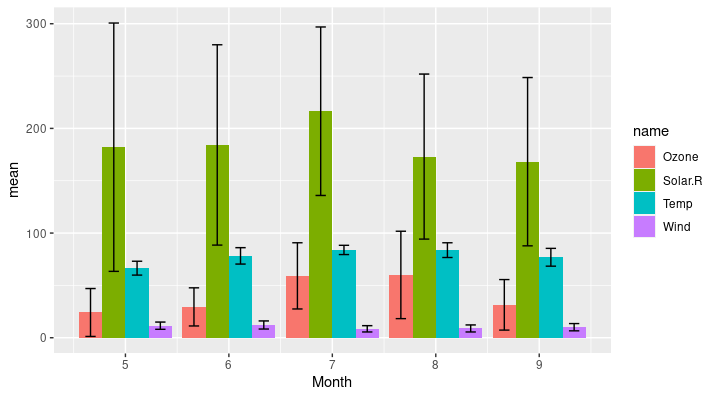
\includegraphics[width=3.64583in,height=\textheight]{images/08/Rplot02.png}

\texttt{ggplot2}를 이용한 그래프 그리기는 다음 시간에 학습하겠습니다.

\hypertarget{ex8.3.1}{%
\subsection{Exercise}\label{ex8.3.1}}

\begin{enumerate}
\def\labelenumi{\arabic{enumi}.}
\item
  InsectSprays 데이터는 살충제 6종에 대한 살충력을 (죽은 벌래의 마릿수) 나타내는 데이터이다. 각 살충제별로 평균과 표준편차를 구하시오
\item
  dplyr 패키지의 starwars 는 스타워즈 영화에 나오는 등장인물들을 분석한 데이터셋 이다. 종족에 따른 키의 평균과 표준편차를 구하시오. (NA 데이터는 제외하고 분석)
\end{enumerate}

\begin{center}\rule{0.5\linewidth}{0.5pt}\end{center}

이 저작물은 크리에이티브 커먼즈 저작자표시-비영리-변경금지 4.0 국제 라이선스에 따라 이용할 수 있습니다.

\hypertarget{ggplot2-for-data-visualization}{%
\chapter{ggplot2 for data visualization}\label{ggplot2-for-data-visualization}}

본 장에서는 \texttt{ggplot2}( \url{https://ggplot2.tidyverse.org/} )를 이용한 시각화에 대해서 알아봅니다. 데이터를 분석할 때 실제 데이터를 눈으로 확인하는 것은 중요합니다. 가능하면 raw 데이터를 보면서 크기 비교나 분포를 대략적으로 예측한다면 tool을 사용해서 나오는 결과를 가늠하는 척도가 될 수도 있습니다. \texttt{ggplot2} 는 Rstudio 개발팀의 해들리위컴이 (Hadley Wickham) 중심이 되어 만든 데이터 시각화 패키지입니다. 몇 가지 새로운 규칙을 학습해야 하지만 그 활용성이나 성능을 고려한다면 꼭 배워야할 패키지 중 하나입니다.

\hypertarget{basics}{%
\section{Basics}\label{basics}}

\texttt{iris} 데이터를 이용해서 간단하게 barplot을 그려봅니다. \texttt{iris} 데이터는 3가지 품종별 꽃잎과 꽃받침의 길이와 넓이를 측정한 데이터 입니다. 다음은 꽃잎의 길이와 넓이의 관계를 볼 수 있는 산점도 입니다.

\begin{Shaded}
\begin{Highlighting}[]
\FunctionTok{library}\NormalTok{(ggplot2)}
\FunctionTok{head}\NormalTok{(iris)}
\FunctionTok{ggplot}\NormalTok{(}\AttributeTok{data=}\NormalTok{iris) }\SpecialCharTok{+}
  \FunctionTok{geom\_point}\NormalTok{(}\AttributeTok{mapping=}\FunctionTok{aes}\NormalTok{(}\AttributeTok{x=}\NormalTok{Petal.Length, }\AttributeTok{y=}\NormalTok{Petal.Width))}
\end{Highlighting}
\end{Shaded}

눈에 띄이는 부분은 \texttt{+}를 이용한 레이어들의 연결입니다. \texttt{ggplot()} 함수 뒤에 다양한 레이어들을 연결할 수 있고 \texttt{geom\_point()} 함수는 지정한 위치에 산점도 레이어를 추가하는 기능을 합니다. 각 레이어들은 다음과 같은 다양한 기능을 갖는 함수들로 구성될 수 있습니다.

\begin{itemize}
\tightlist
\item
  데이터 지정 (ggplot)
\item
  색상, 크기, x축의 값, y축의 값 등 심미적 요소 지정 (aes)
\item
  점, 선, 면 등 기하학적 요소 지정 (geoms)
\item
  그릴 통계량 지정 (stats)
\item
  테마, 스케일 지정 (theme)
\end{itemize}

일반적으로 \texttt{ggplot}을 이용하여 그래프를 그리는 순서는 다음과 같습니다.

\begin{itemize}
\tightlist
\item
  어떤 그래프를 그릴지 결정
\item
  ggplot의 데이터셋과 aesthetic 설정
\item
  geometric 요소와 적절한 statistics를 설정한 레이어 추가
\item
  스케일과 테마를 설정한 레이어 추가
\end{itemize}

ggplot만을 실행할 경우 데이터와 x, y 축만 지정한 상태로 어떤 그래프 (히스토그램인지, 산포도인지 등)를 그릴지 명시되어 있지 않아서 아무것도 그리지 않은 상태의 빈 켄버스만 그려지게 되며 \texttt{geom\_point()} 함수를 즉, 점을 그릴지 선을 그릴지 어떤 통계량을 그릴지 아니면 값 자체를 그릴지 등을 지정해 주고 나서야 비로서 그래프가 그려집니다.

\begin{Shaded}
\begin{Highlighting}[]
\FunctionTok{ggplot}\NormalTok{(}\AttributeTok{data=}\NormalTok{iris, }\AttributeTok{mapping=}\FunctionTok{aes}\NormalTok{(}\AttributeTok{x=}\NormalTok{Petal.Length, }\AttributeTok{y=}\NormalTok{Petal.Width))}
\NormalTok{?ggplot}
\FunctionTok{ggplot}\NormalTok{(iris, }\FunctionTok{aes}\NormalTok{(}\AttributeTok{x=}\NormalTok{Petal.Length, }\AttributeTok{y=}\NormalTok{Petal.Width))}
\FunctionTok{ggplot}\NormalTok{(iris, }\FunctionTok{aes}\NormalTok{(}\AttributeTok{x=}\NormalTok{Petal.Length, }\AttributeTok{y=}\NormalTok{Petal.Width)) }\SpecialCharTok{+} \FunctionTok{geom\_point}\NormalTok{()}
\end{Highlighting}
\end{Shaded}

\texttt{geom\_point()}의 도움말을 보면 다음과 같이 \texttt{data}, \texttt{mapping}, \texttt{stat} 등의 파라메터들이 있습니다. 이는 \texttt{ggplot}함수에서 설정한 \texttt{data}나 \texttt{mapping} 정보를 \texttt{geom\_point}에서 설정 하거나 완전히 다른 데이터를 x축과 y축에 그릴 수 있다는 뜻 이기도 합니다.

\begin{Shaded}
\begin{Highlighting}[]
\FunctionTok{ggplot}\NormalTok{() }\SpecialCharTok{+} 
  \FunctionTok{geom\_point}\NormalTok{(}\AttributeTok{data=}\NormalTok{iris, }\AttributeTok{mapping=}\FunctionTok{aes}\NormalTok{(}\AttributeTok{x=}\NormalTok{Petal.Length, }\AttributeTok{y=}\NormalTok{Petal.Width)) }
\end{Highlighting}
\end{Shaded}

그런데 위 꽃잎의 길이와 넓이는 세 가지 다른 종류의 붓꽃에 대한 정보입니다. 따라서 각 종에 따라 다른 색이나 기호를 할당하는 것도 \texttt{mapping}에서 설정할 수 있습니다.

\begin{Shaded}
\begin{Highlighting}[]
\FunctionTok{ggplot}\NormalTok{(iris, }\FunctionTok{aes}\NormalTok{(}\AttributeTok{x=}\NormalTok{Petal.Length, }
                 \AttributeTok{y=}\NormalTok{Petal.Width, }
                 \AttributeTok{color=}\NormalTok{Species, }
                 \AttributeTok{shape=}\NormalTok{Species)) }\SpecialCharTok{+} 
  \FunctionTok{geom\_point}\NormalTok{()}

\FunctionTok{ggplot}\NormalTok{(iris, }\FunctionTok{aes}\NormalTok{(}\AttributeTok{x=}\NormalTok{Petal.Length, }\AttributeTok{y=}\NormalTok{Petal.Width)) }\SpecialCharTok{+} 
  \FunctionTok{geom\_point}\NormalTok{(}\FunctionTok{aes}\NormalTok{(}\AttributeTok{color=}\NormalTok{Species, }\AttributeTok{shape=}\NormalTok{Species))}
\end{Highlighting}
\end{Shaded}

위 산점도들의 \texttt{stat}은 \texttt{identity} 입니다. 즉, 따로 통계량을 계산할 필요 없이 값 그 자체를 사용하겠다는 것 입니다. 히스토그램의 경우 \texttt{geom\_bar()} 함수로 막대그래프를 그릴 수 있습니다. \texttt{geom\_bar}의 help페이지를 보면 \texttt{stat="count"}로 설정되어 있는 것을 알 수 있습니다. 꽃잎의 넓이에 대한 분포를 예로 구해봅니다. 히스토그램을 그릴경우 변수 한 개의 데이터만 필요하고 y축에는 자동으로 빈도수가 들어가게 되므로 \texttt{aes}에서 x만 mapping 해 주면 됩니다.

\begin{Shaded}
\begin{Highlighting}[]
\FunctionTok{ggplot}\NormalTok{(iris, }\FunctionTok{aes}\NormalTok{(}\AttributeTok{x=}\NormalTok{Petal.Width)) }\SpecialCharTok{+}  
  \FunctionTok{geom\_bar}\NormalTok{()}
\end{Highlighting}
\end{Shaded}

\hypertarget{bar-graph}{%
\section{Bar graph}\label{bar-graph}}

ggplot을 이용한 막대그래프 그리는 방법에 대해서 좀 더 알아보겠습니다. 앞서와 같이 ggplot 함수로 먼저 데이터와 aes로 x축 y축 등을 명시하고 \texttt{+} 오퍼레이터를 사용하여 필요한 레이어를 차례로 추가하면서 그래프를 그릴 수 있습니다. \texttt{geom\_bar()} 함수의 경우 x가 연속형일 경우는 아래와 같이 히스토그램을 그려주기 어렵습니다 (위 iris 예제에서 \texttt{geom\_bar()} 그래프에서는 실제 꽃받침의 width 값은 연속형이 맞으나 관측된 iris 데이터들이 같은 값들이 많은 범주형처럼 되어 있어 히스토그램 그림이 그려졌습니다) 이럴 경우 stat을 \texttt{bin}으로 바꿔주면 해당 범위 안에 있는 값들의 빈도수를 계산하여 히스토그램을 그릴 수 있습니다.

\begin{Shaded}
\begin{Highlighting}[]
\NormalTok{dat }\OtherTok{\textless{}{-}} \FunctionTok{data.frame}\NormalTok{(}\AttributeTok{x1=}\FunctionTok{rnorm}\NormalTok{(}\DecValTok{100}\NormalTok{))}
\FunctionTok{ggplot}\NormalTok{(dat, }\FunctionTok{aes}\NormalTok{(}\AttributeTok{x=}\NormalTok{x1)) }\SpecialCharTok{+}
  \FunctionTok{geom\_bar}\NormalTok{()}

\FunctionTok{ggplot}\NormalTok{(dat, }\FunctionTok{aes}\NormalTok{(}\AttributeTok{x=}\NormalTok{x1)) }\SpecialCharTok{+}
  \FunctionTok{geom\_bar}\NormalTok{(}\AttributeTok{stat=}\StringTok{"bin"}\NormalTok{, }\AttributeTok{bins=}\DecValTok{30}\NormalTok{)}
\end{Highlighting}
\end{Shaded}

x가 이산형인 경우는 stat을 디폴트 값인 \texttt{count}로 설정하여 해당 값들의 빈도수를 그려줄 수 있습니다. 이는 앞서 \texttt{iris}에서 배운 예제와 같습니다.

\begin{Shaded}
\begin{Highlighting}[]
\NormalTok{x1 }\OtherTok{\textless{}{-}} \FunctionTok{sample}\NormalTok{(}\DecValTok{1}\SpecialCharTok{:}\DecValTok{4}\NormalTok{, }\DecValTok{100}\NormalTok{, }\AttributeTok{replace =}\NormalTok{ T)}
\NormalTok{dat }\OtherTok{\textless{}{-}} \FunctionTok{data.frame}\NormalTok{(}\AttributeTok{x=}\NormalTok{x1)}
\FunctionTok{ggplot}\NormalTok{(dat, }\FunctionTok{aes}\NormalTok{(}\AttributeTok{x=}\NormalTok{x)) }\SpecialCharTok{+}
  \FunctionTok{geom\_bar}\NormalTok{(}\AttributeTok{stat=}\StringTok{"count"}\NormalTok{)}
\end{Highlighting}
\end{Shaded}

이제 두 개의 변수가 있는 경우를 생각해 봅니다. 두 변수에 대해서 막대그래프를 그릴 경우 다음과 같이 \texttt{Error:\ stat\_count()\ must\ not\ be\ used\ with\ a\ y\ aesthetic.} 에러가 발생할 수 있습니다.

\begin{Shaded}
\begin{Highlighting}[]
\NormalTok{x1 }\OtherTok{\textless{}{-}} \FunctionTok{rnorm}\NormalTok{(}\DecValTok{10}\NormalTok{)}
\NormalTok{x2 }\OtherTok{\textless{}{-}} \FunctionTok{rnorm}\NormalTok{(}\DecValTok{10}\NormalTok{)}
\NormalTok{dat }\OtherTok{\textless{}{-}} \FunctionTok{data.frame}\NormalTok{(x1, x2)}
\FunctionTok{ggplot}\NormalTok{(dat, }\FunctionTok{aes}\NormalTok{(}\AttributeTok{x=}\NormalTok{x1, }\AttributeTok{y=}\NormalTok{x2)) }\SpecialCharTok{+}
  \FunctionTok{geom\_bar}\NormalTok{()}
\end{Highlighting}
\end{Shaded}

이는 \texttt{geom\_bar()}의 \texttt{stat}이 기본적으로 \texttt{count}로 설정되어 있으므로 생기는 에러 입니다. \texttt{stat}을 \texttt{identity}로 설정하면 x1값에 해당하는 x2값을 그려주는 막대 그래프를 그릴 수 있습니다. 참고로 이 그래프는 \texttt{geom\_point}와 비슷한 정보를 보여 주게 됩니다.

\begin{Shaded}
\begin{Highlighting}[]
\NormalTok{x1 }\OtherTok{\textless{}{-}} \FunctionTok{rnorm}\NormalTok{(}\DecValTok{10}\NormalTok{)}
\NormalTok{x2 }\OtherTok{\textless{}{-}} \FunctionTok{rnorm}\NormalTok{(}\DecValTok{10}\NormalTok{)}
\NormalTok{dat }\OtherTok{\textless{}{-}} \FunctionTok{data.frame}\NormalTok{(x1, x2)}
\FunctionTok{ggplot}\NormalTok{(dat, }\FunctionTok{aes}\NormalTok{(}\AttributeTok{x=}\NormalTok{x1, }\AttributeTok{y=}\NormalTok{x2)) }\SpecialCharTok{+}
  \FunctionTok{geom\_bar}\NormalTok{(}\AttributeTok{stat=}\StringTok{"identity"}\NormalTok{)}

\FunctionTok{ggplot}\NormalTok{(dat, }\FunctionTok{aes}\NormalTok{(}\AttributeTok{x=}\NormalTok{x1, }\AttributeTok{y=}\NormalTok{x2)) }\SpecialCharTok{+}
  \FunctionTok{geom\_point}\NormalTok{()}
\end{Highlighting}
\end{Shaded}

다음과 같이 레이어를 추가하여 두 그래프를 같은 화면에 그릴 수도 있습니다. 여기서 \texttt{col}과 \texttt{size}는 \texttt{aes}함수안에서 쓰이지 않았음을 주의하시기 바랍니다. \texttt{aes}에서는 데이터와 특정 모양, 색깔을 mapping 해주는 역할을 하고 아래와 같이 지정해 줄 경우 데이터와 상관 없이 해당 레이어의 모든 그래프에 대해서 일괄적으로 적용되게 됩니다.

\begin{Shaded}
\begin{Highlighting}[]
\FunctionTok{ggplot}\NormalTok{(dat, }\FunctionTok{aes}\NormalTok{(}\AttributeTok{x=}\NormalTok{x1, }\AttributeTok{y=}\NormalTok{x2)) }\SpecialCharTok{+}
  \FunctionTok{geom\_bar}\NormalTok{(}\AttributeTok{stat=}\StringTok{"identity"}\NormalTok{) }\SpecialCharTok{+}
  \FunctionTok{geom\_point}\NormalTok{(}\AttributeTok{col=}\StringTok{"red"}\NormalTok{, }\AttributeTok{size=}\DecValTok{5}\NormalTok{)}
\end{Highlighting}
\end{Shaded}

또한 다음과 같이 다양한 레이어를 추가하여 필요한 기능을 사용할 수 있습니다. \texttt{fill=x1} 이라는 코드는 막대그래프의 색을 채울 때 x1에 따라서 다른 값들을 채우는 역할을 한다고 보면 되겠습니다.

\begin{Shaded}
\begin{Highlighting}[]
\NormalTok{x1 }\OtherTok{\textless{}{-}} \FunctionTok{as.factor}\NormalTok{(}\DecValTok{1}\SpecialCharTok{:}\DecValTok{3}\NormalTok{)}
\NormalTok{y1 }\OtherTok{\textless{}{-}} \FunctionTok{tabulate}\NormalTok{(}\FunctionTok{sample}\NormalTok{(x1, }\DecValTok{100}\NormalTok{, }\AttributeTok{replace=}\NormalTok{T))}
\NormalTok{dat }\OtherTok{\textless{}{-}} \FunctionTok{data.frame}\NormalTok{(x1, y1)}
\FunctionTok{ggplot}\NormalTok{(dat, }\FunctionTok{aes}\NormalTok{(}\AttributeTok{x=}\NormalTok{x1, }\AttributeTok{y=}\NormalTok{y1, }\AttributeTok{fill=}\NormalTok{x1)) }\SpecialCharTok{+}
  \FunctionTok{geom\_bar}\NormalTok{(}\AttributeTok{stat=}\StringTok{"identity"}\NormalTok{) }\SpecialCharTok{+}
  \FunctionTok{guides}\NormalTok{(}\AttributeTok{fill=}\ConstantTok{FALSE}\NormalTok{) }\SpecialCharTok{+}
  \FunctionTok{xlab}\NormalTok{(}\StringTok{"Discrete cases"}\NormalTok{) }\SpecialCharTok{+} 
  \FunctionTok{ylab}\NormalTok{(}\StringTok{"Value"}\NormalTok{) }\SpecialCharTok{+}
  \FunctionTok{ylim}\NormalTok{(}\FunctionTok{c}\NormalTok{(}\DecValTok{0}\NormalTok{,}\DecValTok{50}\NormalTok{))}\SpecialCharTok{+}
  \FunctionTok{ggtitle}\NormalTok{(}\StringTok{"Bar graph for x:discrete and y:value"}\NormalTok{)}
\end{Highlighting}
\end{Shaded}

\hypertarget{line-graph}{%
\section{Line graph}\label{line-graph}}

다음으로 ggplot을 이용한 line graph를 그리는 방법을 알아 봅니다. Line graph는 geom\_line이라는 함수를 사용해서 그릴 수 있으며 stat의 사용법은 앞서 bar graph와 같습니다.

\begin{Shaded}
\begin{Highlighting}[]
\NormalTok{x1 }\OtherTok{\textless{}{-}} \FunctionTok{c}\NormalTok{(}\DecValTok{12}\NormalTok{, }\DecValTok{21}\NormalTok{, }\DecValTok{40}\NormalTok{)}
\NormalTok{x2 }\OtherTok{\textless{}{-}} \FunctionTok{c}\NormalTok{(}\DecValTok{33}\NormalTok{, }\DecValTok{10}\NormalTok{, }\DecValTok{82}\NormalTok{)}
\NormalTok{dat }\OtherTok{\textless{}{-}} \FunctionTok{data.frame}\NormalTok{(x1, x2)}
\FunctionTok{ggplot}\NormalTok{(dat, }\FunctionTok{aes}\NormalTok{(x1, x2)) }\SpecialCharTok{+}
  \FunctionTok{geom\_line}\NormalTok{()}
\end{Highlighting}
\end{Shaded}

아래와 같이 그려지는 선의 두께를 조절하거나 레이어를 추가하는 방법으로 점을 추가로 그려볼 수 있습니다. \texttt{fill}의 경우 특정 도형에 채워지는 색을 의미합니다. 도형에 대한 자세한 종류는 \texttt{?pch} 라는 도움말로 살펴보실 수 있습니다.

\begin{Shaded}
\begin{Highlighting}[]
\FunctionTok{ggplot}\NormalTok{(dat, }\FunctionTok{aes}\NormalTok{(}\AttributeTok{x=}\NormalTok{x1, }\AttributeTok{y=}\NormalTok{x2)) }\SpecialCharTok{+}
  \FunctionTok{geom\_line}\NormalTok{(}\AttributeTok{size=}\DecValTok{2}\NormalTok{) }\SpecialCharTok{+}
  \FunctionTok{geom\_point}\NormalTok{(}\AttributeTok{size=}\DecValTok{4}\NormalTok{, }\AttributeTok{pch=}\DecValTok{21}\NormalTok{, }\AttributeTok{fill=}\StringTok{"white"}\NormalTok{) }\SpecialCharTok{+}
  \FunctionTok{guides}\NormalTok{(}\AttributeTok{fill=}\ConstantTok{FALSE}\NormalTok{) }\SpecialCharTok{+}
  \FunctionTok{ylim}\NormalTok{(}\FunctionTok{c}\NormalTok{(}\DecValTok{0}\NormalTok{, }\DecValTok{100}\NormalTok{)) }\SpecialCharTok{+}
  \FunctionTok{xlab}\NormalTok{(}\StringTok{"Continuous cases"}\NormalTok{) }\SpecialCharTok{+} \FunctionTok{ylab}\NormalTok{(}\StringTok{"Value"}\NormalTok{) }\SpecialCharTok{+}
  \FunctionTok{ggtitle}\NormalTok{(}\StringTok{"Line graph for x:continuous and y:continuous"}\NormalTok{)}
\end{Highlighting}
\end{Shaded}

위 경우는 x와 y가 모두 연속형 데이터일 경우 입니다. x는 이산형, y가 연속형일 경우 앞에서와 같이 bar graph를 이용하여 그래프를 그리게 됩니다. 그런데 이런 bar의 높이에 해당하는 값들을 서로 선으로 연결하고 싶은 경우가 있습니다. 이 때는 다음과 같이 \texttt{aes}의 \texttt{group} 이라는 파라미터를 설정하여 두 점 이상을 연결할 수 있습니다. 만약 group으로 나타낼 수 있는 변수가 없을 경우 \texttt{group=1}이라고 명시해 주고 선을 그릴 수 있으며 이 경우 모든 값들이 같은 \texttt{1} 그룹에 있는 것으로 간주됩니다. \texttt{1}이라는 것은 하나의 예이며 어떤 숫자나 문자가 와도 괜찮습니다.

\begin{Shaded}
\begin{Highlighting}[]
\NormalTok{x1 }\OtherTok{\textless{}{-}} \FunctionTok{as.factor}\NormalTok{(}\FunctionTok{c}\NormalTok{(}\DecValTok{1}\SpecialCharTok{:}\DecValTok{3}\NormalTok{))}
\NormalTok{y1 }\OtherTok{\textless{}{-}} \FunctionTok{c}\NormalTok{(}\DecValTok{33}\NormalTok{, }\DecValTok{10}\NormalTok{, }\DecValTok{82}\NormalTok{)}
\NormalTok{dat }\OtherTok{\textless{}{-}} \FunctionTok{data.frame}\NormalTok{(x1, y1)}
\FunctionTok{str}\NormalTok{(dat)}
\FunctionTok{ggplot}\NormalTok{(dat, }\FunctionTok{aes}\NormalTok{(}\AttributeTok{x=}\NormalTok{x1, }\AttributeTok{y=}\NormalTok{y1, }\AttributeTok{group=}\DecValTok{1}\NormalTok{)) }\SpecialCharTok{+}
  \FunctionTok{geom\_line}\NormalTok{(}\AttributeTok{stat=}\StringTok{"identity"}\NormalTok{) }\SpecialCharTok{+}
  \FunctionTok{guides}\NormalTok{(}\AttributeTok{fill=}\ConstantTok{FALSE}\NormalTok{) }\SpecialCharTok{+}
  \FunctionTok{xlab}\NormalTok{(}\StringTok{"Discrete cases"}\NormalTok{) }\SpecialCharTok{+} \FunctionTok{ylab}\NormalTok{(}\StringTok{"Value"}\NormalTok{) }\SpecialCharTok{+}
  \FunctionTok{ylim}\NormalTok{(}\FunctionTok{c}\NormalTok{(}\DecValTok{0}\NormalTok{,}\DecValTok{100}\NormalTok{))}\SpecialCharTok{+}
  \FunctionTok{ggtitle}\NormalTok{(}\StringTok{"Line plot for x:discrete and y:continuous"}\NormalTok{)}
\end{Highlighting}
\end{Shaded}

위에서와 같은 방법으로 point와 bar 등을 같이 그려줄 수 있습니다.

\begin{Shaded}
\begin{Highlighting}[]
\FunctionTok{ggplot}\NormalTok{(dat, }\FunctionTok{aes}\NormalTok{(}\AttributeTok{x=}\NormalTok{x1, }\AttributeTok{y=}\NormalTok{y1, }\AttributeTok{group=}\DecValTok{1}\NormalTok{)) }\SpecialCharTok{+}
  \FunctionTok{geom\_bar}\NormalTok{(}\AttributeTok{stat=}\StringTok{"identity"}\NormalTok{, }\AttributeTok{fill=}\NormalTok{x1) }\SpecialCharTok{+}
  \FunctionTok{geom\_line}\NormalTok{(}\AttributeTok{size=}\DecValTok{2}\NormalTok{) }\SpecialCharTok{+}
  \FunctionTok{geom\_point}\NormalTok{(}\AttributeTok{size=}\DecValTok{4}\NormalTok{, }\AttributeTok{pch=}\DecValTok{21}\NormalTok{, }\AttributeTok{fill=}\StringTok{"white"}\NormalTok{) }\SpecialCharTok{+}
  \FunctionTok{guides}\NormalTok{(}\AttributeTok{fill=}\ConstantTok{FALSE}\NormalTok{) }\SpecialCharTok{+}
  \FunctionTok{xlab}\NormalTok{(}\StringTok{"Discrete cases"}\NormalTok{) }\SpecialCharTok{+} \FunctionTok{ylab}\NormalTok{(}\StringTok{"Value"}\NormalTok{) }\SpecialCharTok{+}
  \FunctionTok{ylim}\NormalTok{(}\FunctionTok{c}\NormalTok{(}\DecValTok{0}\NormalTok{,}\DecValTok{100}\NormalTok{))}\SpecialCharTok{+}
  \FunctionTok{ggtitle}\NormalTok{(}\StringTok{"Line for x:discrete and y:value"}\NormalTok{)}
\end{Highlighting}
\end{Shaded}

여기서는 fill 옵션이 geom\_bar에 하나 geom\_point에 하나씩 쓰였는데 geom\_bar에서 사용된 fill은 bar에 채워지는 색을 x1의 값에 따라 바꾸겠다는 것을 의미하고 \texttt{geom\_point}의 fill은 데이터에 상관 없이 모두 white로 채우라는 명령 입니다. 각 geometry에 따라서 필요한 옵션이 다르므로 각각의 geom\_xxx를 사용할 때 상황에 맞게 사용하시면 되겠습니다.

\hypertarget{smoothing}{%
\section{Smoothing}\label{smoothing}}

산포도는 앞서와 같이 데이터를 점으로 표현한 그래프입니다. Smoothing은 관측된 데이터를 이용하여 모형을 추정하는데 사용되는 통계적 방법이며 이를 그래프로 표현하여 추세선을 그릴 수 있습니다. 예를 들어 몸무게와 키라는 두 변수의 관계를 알아보고자 할 때 산포도를 그리고 Smoothing을 통해 점들의 평균값을 이어주는 방법으로 모형을 추정하고 추세선을 그릴 수 있습니다.

\texttt{mtcars} 데이터는 1974년 미국 자동차 잡지에서 추출한 데이터로서 당시 다양한 모델의 자동차에대한 성능을 저장하고 있습니다 (\texttt{?mtcars}로 자세한 정보를 볼 수 있음). 이 데이터를 이용해서 연비와 마력 (horsepower) 두 변수의 관계를 그래프로 그려보겠습니다. 직관적으로 생각하면 두 변수는 반비례 할 것으로 기대됩니다. \texttt{ggplot}을 활용해서 두 변수의 산포도를 그리고 smoothing을 수행해 보도록 하겠습니다.

\begin{Shaded}
\begin{Highlighting}[]
\FunctionTok{ggplot}\NormalTok{(mtcars, }\FunctionTok{aes}\NormalTok{(}\AttributeTok{x=}\NormalTok{mpg, }\AttributeTok{y=}\NormalTok{hp)) }\SpecialCharTok{+}
  \FunctionTok{geom\_point}\NormalTok{()}
\end{Highlighting}
\end{Shaded}

위와 같이 \texttt{mtcars}는 \texttt{data.frame}이므로 \texttt{ggplot}으로 바로 받아서 x축과 y축 mapping에 필요한 변수들 이름을 직접 할당하고 \texttt{geom\_point}함수를 이용해서 간단히 산포도를 그릴 수 있습니다. 이 산포도만으로도 mpg와 hp 두 변수간의 관계가 역함수 관계임을 알 수 있고 또한 선형이 아닌 것도 알 수 있습니다. 이제 위 그림에 \texttt{geom\_smooth()}함수를 이용해서 (모형) 적합 곡선 (또는 추세선)을 그려봅니다.

\begin{Shaded}
\begin{Highlighting}[]
\FunctionTok{ggplot}\NormalTok{(mtcars, }\FunctionTok{aes}\NormalTok{(}\AttributeTok{x=}\NormalTok{mpg, }\AttributeTok{y=}\NormalTok{hp)) }\SpecialCharTok{+}
  \FunctionTok{geom\_point}\NormalTok{() }\SpecialCharTok{+}
  \FunctionTok{geom\_smooth}\NormalTok{()}
\end{Highlighting}
\end{Shaded}

간단히 \texttt{geom\_smooth()} 한 줄을 추가하여 추세선을 그렸으며 경고 메세지에서 볼 수 있듯이 알고리즘은 \texttt{loess} 모형을 사용했고 공식은 (formula는) \texttt{y\textasciitilde{}x}로, 즉, y축 변수를 반응변수로 x축 변수를 설명변수로 설정하여 그려졌습니다. 직선의 공식 \texttt{y=ax+b}를 생각해 보시면 무슨 의미인지 이해가 더 쉬울듯 합니다. \texttt{?geom\_smooth}로 보면 알 수 있듯이 모형을 적합하는 알고리즘 옵션을 \texttt{lm}, \texttt{glm}, \texttt{loess} 등 다양하게 설정할 수 있으며 \texttt{auto}로 하게 되면 데이터의 크기나 형식에 맞춰서 방법을 자동으로 선택해서 그려주게 됩니다. \texttt{se} 옵션은 기본적으로 \texttt{TRUE} 값을 가지며 위 그림에서 볼 수 있는 선분 주위의 회색 구간으로 신뢰구간을 그려주는 옵션 입니다. \texttt{span} 옵션은 loess 모형의 smoothing 정도를 조절할 수 있는데 이는 직접 바꿔가면서 실습을 해보면 이해에 도움이 되겠습니다.

\begin{Shaded}
\begin{Highlighting}[]
\FunctionTok{ggplot}\NormalTok{(mtcars, }\FunctionTok{aes}\NormalTok{(}\AttributeTok{x=}\NormalTok{mpg, }\AttributeTok{y=}\NormalTok{hp)) }\SpecialCharTok{+}
  \FunctionTok{geom\_point}\NormalTok{() }\SpecialCharTok{+}
  \FunctionTok{geom\_smooth}\NormalTok{(}\AttributeTok{se=}\ConstantTok{FALSE}\NormalTok{, }\AttributeTok{span=}\FloatTok{0.2}\NormalTok{)}
\end{Highlighting}
\end{Shaded}

위와 같이 \texttt{span} 옵션을 작게 설정할 수록 관측된 데이터(점)에 선분(모형)이 가까이 붙게 됩니다. 이를 과대적합 (overfitting)이라고 하며 간단히 설명하면 관측된 데이터에만 너무 잘맞는 모형을 만드는 경우를 말합니다. 이럴 경우 새롭게 관측된 데이터는 모형의 예측값과 잘 맞지 않게 됩니다.

이번에는 모의 데이터를 생성해서 그래프를 그려보겠습니다. 네 개 학급에 있는 학생들의 키와 몸무게를 저장한 데이터를 만들어 봅니다. 이 경우 몇 개의 변수가 필요할지 생각해 보시기 바랍니다. 키와 몸무게 그리고 학급을 나타내는 변수 3개가 필요하며 키와 몸무게는 정수형, 그룹을 나타내는 변수는 문자형이나 factor형으로 나타내면 되겠습니다. 각 학급의 학생수는 50명으로 총 200명의 학생이 있는 것으로 하며 각 그룹별로 키나 몸무게의 차이는 없고 키가 큰 사람은 몸무게가 많이 나가는 것으로 합니다. 키와 몸무게 사이에는 다음과 같은 연관성을 만들어 줍니다. \(height= weight + N(100, 10)\)

\begin{Shaded}
\begin{Highlighting}[]
\NormalTok{weights }\OtherTok{\textless{}{-}} \FunctionTok{rnorm}\NormalTok{(}\DecValTok{200}\NormalTok{, }\DecValTok{75}\NormalTok{, }\DecValTok{5}\NormalTok{)}
\NormalTok{heights }\OtherTok{\textless{}{-}}\NormalTok{ weights }\SpecialCharTok{+} \FunctionTok{rnorm}\NormalTok{(}\DecValTok{200}\NormalTok{, }\DecValTok{100}\NormalTok{, }\DecValTok{5}\NormalTok{)}
\NormalTok{classes }\OtherTok{\textless{}{-}} \FunctionTok{sample}\NormalTok{(}\FunctionTok{c}\NormalTok{(}\StringTok{"A"}\NormalTok{, }\StringTok{"B"}\NormalTok{, }\StringTok{"C"}\NormalTok{, }\StringTok{"D"}\NormalTok{), }\AttributeTok{size=}\FunctionTok{length}\NormalTok{(heights), }\AttributeTok{replace =}\NormalTok{ T)}
\NormalTok{mydata }\OtherTok{\textless{}{-}} \FunctionTok{data.frame}\NormalTok{(heights, weights, classes)}
\FunctionTok{str}\NormalTok{(mydata)}
\end{Highlighting}
\end{Shaded}

이제 위 데이터를 이용해서 몸무게와 키의 산포도와 추세선을 그려보고 추가로 그룹별로 다른 색의 점으로 표현해 보겠습니다.

\begin{Shaded}
\begin{Highlighting}[]
\FunctionTok{ggplot}\NormalTok{(mydata, }\FunctionTok{aes}\NormalTok{(}\AttributeTok{x=}\NormalTok{weights, }\AttributeTok{y=}\NormalTok{heights, }\AttributeTok{color=}\NormalTok{classes)) }\SpecialCharTok{+}
  \FunctionTok{geom\_point}\NormalTok{() }\SpecialCharTok{+}
  \FunctionTok{geom\_smooth}\NormalTok{()}
\end{Highlighting}
\end{Shaded}

그런데 위와 같은 코드를 실행하면 그룹마다 다른 점과 smooth 선분이 그려집니다. 우리가 원하는 그림은 단지 점만 그룹별로 다른 색으로 표현하고 추세선은 전체 학생들에 대해서 하나의 선분만 그려지길 원합니다. 이제 우리가 알아야할 부분은 각 레이어마다 mapping을 지정할 수 있다는 것이고 이 원리를 이해한다면 다음과 같이 \texttt{geom\_point}에서는 \texttt{color}를 mapping해 주고 \texttt{geom\_smooth}에서는 지정해주지 않으면 됩니다.

\begin{Shaded}
\begin{Highlighting}[]
\FunctionTok{ggplot}\NormalTok{(mydata) }\SpecialCharTok{+}
  \FunctionTok{geom\_point}\NormalTok{(}\FunctionTok{aes}\NormalTok{(}\AttributeTok{x=}\NormalTok{weights, }\AttributeTok{y=}\NormalTok{heights, }\AttributeTok{color=}\NormalTok{classes)) }\SpecialCharTok{+}
  \FunctionTok{geom\_smooth}\NormalTok{(}\FunctionTok{aes}\NormalTok{(}\AttributeTok{x=}\NormalTok{weights, }\AttributeTok{y=}\NormalTok{heights))}
\end{Highlighting}
\end{Shaded}

그리고 중복되는 부분을 줄여줄 수도 있습니다. 즉, ggplot에서 지정하는 mapping은 하위 layer에 모두 적용이 되며 각 layer마다 다른 mapping 특성을 부여하고 싶을 경우 해당 layer의 mapping 함수 (aes)를 이용하여 설정할 수 있다는 점을 기억하시기 바랍니다.

\begin{Shaded}
\begin{Highlighting}[]
\FunctionTok{ggplot}\NormalTok{(mydata, }\FunctionTok{aes}\NormalTok{(}\AttributeTok{x=}\NormalTok{weights, }\AttributeTok{y=}\NormalTok{heights)) }\SpecialCharTok{+}
  \FunctionTok{geom\_point}\NormalTok{(}\FunctionTok{aes}\NormalTok{(}\AttributeTok{color=}\NormalTok{classes)) }\SpecialCharTok{+}
  \FunctionTok{geom\_smooth}\NormalTok{()}
\end{Highlighting}
\end{Shaded}

\hypertarget{statstics-and-positions}{%
\section{Statstics and positions}\label{statstics-and-positions}}

앞서 smoothing 곡선은 실제 데이터에서 관측된 값이 아닌 계산된 값을 그래프에 표현한 것 입니다. 막대그래프에서도 y축 count 값은 관측된 값이 아닌 빈도수를 계산한 값이고 boxplot의 경우도 중간값 1,3사분위수 등 통계량을 표현해 주는 그래프 입니다. 이는 대부분 통계 분석용 소프트웨어에서 제공되는 기능으로 통계량을 가시화 해주는 역할을 합니다. \texttt{ggplot2}에서도 각 geom 레이어에 \texttt{stat}이라는 옵션을 통해 이러한 통계량을 그래프로 표현할 수 있습니다. 예를 들어 앞서 생성한 키, 몸무게 데이터에서 키의 분포를 보기 위한 히스토그램을 그리면 \texttt{geom\_histogram}을 사용할 수 있고 이 레이어의 \texttt{stat} 옵션의 기본값은 \texttt{"bin"} 입니다 (\texttt{?geom\_histogram} 참고).

\begin{Shaded}
\begin{Highlighting}[]
\FunctionTok{library}\NormalTok{(tidyverse)}

\NormalTok{weights }\OtherTok{\textless{}{-}} \FunctionTok{rnorm}\NormalTok{(}\DecValTok{200}\NormalTok{, }\DecValTok{75}\NormalTok{, }\DecValTok{5}\NormalTok{)}
\NormalTok{heights }\OtherTok{\textless{}{-}}\NormalTok{ weights }\SpecialCharTok{+} \FunctionTok{rnorm}\NormalTok{(}\DecValTok{200}\NormalTok{, }\DecValTok{100}\NormalTok{, }\DecValTok{5}\NormalTok{)}
\NormalTok{classes }\OtherTok{\textless{}{-}} \FunctionTok{sample}\NormalTok{(}\FunctionTok{c}\NormalTok{(}\StringTok{"A"}\NormalTok{, }\StringTok{"B"}\NormalTok{, }\StringTok{"C"}\NormalTok{, }\StringTok{"D"}\NormalTok{), }\AttributeTok{size=}\FunctionTok{length}\NormalTok{(heights), }\AttributeTok{replace =}\NormalTok{ T)}
\NormalTok{mydata }\OtherTok{\textless{}{-}} \FunctionTok{data.frame}\NormalTok{(heights, weights, classes)}
\FunctionTok{str}\NormalTok{(mydata)}

\FunctionTok{ggplot}\NormalTok{(mydata, }\FunctionTok{aes}\NormalTok{(}\AttributeTok{x=}\NormalTok{heights)) }\SpecialCharTok{+}
  \FunctionTok{geom\_histogram}\NormalTok{()}
\end{Highlighting}
\end{Shaded}

경고 문구의 \texttt{bins=30}은 기본 \texttt{stat}옵션이 \texttt{bin}인데 \texttt{bins}옵션은 null로 되어 있기 때문에 경고가 발생한 것이고 30으로 강제 할당해서 그린다는 메세지 입니다. bins 옵션을 다르게 해서 테스트 해보시기 바랍니다. 또한 \texttt{stat="identity"}로 그래프를 그린 경우는 데이터 값을 그대로 그린다는 것도 다시 기억해 보시기 바랍니다.

\begin{Shaded}
\begin{Highlighting}[]
\FunctionTok{ggplot}\NormalTok{(mydata, }\FunctionTok{aes}\NormalTok{(}\AttributeTok{x=}\NormalTok{heights)) }\SpecialCharTok{+}
  \FunctionTok{geom\_histogram}\NormalTok{(}\AttributeTok{stat=}\StringTok{"identity"}\NormalTok{)}

\FunctionTok{ggplot}\NormalTok{(mydata, }\FunctionTok{aes}\NormalTok{(}\AttributeTok{x=}\NormalTok{heights, }\AttributeTok{y=}\NormalTok{weights)) }\SpecialCharTok{+}
  \FunctionTok{geom\_histogram}\NormalTok{(}\AttributeTok{stat=}\StringTok{"identity"}\NormalTok{)}
\end{Highlighting}
\end{Shaded}

또 다른 예를위해 앞서 키 몸무게 데이터에 혈액형 변수를 추가해 보겠습니다. 혈액형은 위 4개 학급에 관계 없이 A, B, O, AB 네 그룹으로 나눌 수 있으며 200명의 학생들에게 랜덤하게 할당하도록 합니다.

\begin{Shaded}
\begin{Highlighting}[]
\NormalTok{bloodtype }\OtherTok{\textless{}{-}} \FunctionTok{sample}\NormalTok{(}\FunctionTok{c}\NormalTok{(}\StringTok{"A"}\NormalTok{, }\StringTok{"B"}\NormalTok{, }\StringTok{"O"}\NormalTok{, }\StringTok{"AB"}\NormalTok{), }\FunctionTok{nrow}\NormalTok{(mydata), }\AttributeTok{replace=}\NormalTok{T)}
\NormalTok{mynewdata }\OtherTok{\textless{}{-}} \FunctionTok{data.frame}\NormalTok{(mydata, bloodtype)}
\FunctionTok{str}\NormalTok{(mynewdata)}
\end{Highlighting}
\end{Shaded}

위와 같이 새로운 변수 bloodtype 이 \texttt{factor}형으로 추가되어 새로운 \texttt{data.frame}을 생성하도록 했습니다. 이제 각 학급별로 몇 명의 혈액형 타입을 갖는 학생들이 있는지를 막대그래프로 표현해 보도록 하겠습니다. 혈액형의 타입별로 다른 색으로 막대를 칠하도록 해봅니다. 막대그래프의 색은 \texttt{fill}옵션으로 채울수 있고 막대그래프는 \texttt{geom\_bar}그리고 이 레이어의 \texttt{stat}은 기본값이 \texttt{count}이므로 따로 명시하지 않은채로 다음과 같이 코드를 작성할 수 있습니다.

\begin{Shaded}
\begin{Highlighting}[]
\FunctionTok{ggplot}\NormalTok{(mynewdata, }\FunctionTok{aes}\NormalTok{(}\AttributeTok{x=}\NormalTok{classes, }\AttributeTok{fill=}\NormalTok{bloodtype)) }\SpecialCharTok{+}
  \FunctionTok{geom\_bar}\NormalTok{()}
\end{Highlighting}
\end{Shaded}

그런데 위와같이 그래프가 위로 쌓여서 보입니다. 이는 \texttt{geom\_bar}의 \texttt{position} 기본값이 \texttt{stack}으로 되어있어서 보이는 현상입니다 (\texttt{?geom\_bar}참고). 옆으로 나란히 막대를 위치시킨 후 크기를 비교하기 위해서 \texttt{position="dodge"}를 사용합니다. 또한 막대그래프에 칠해지는 색의 투명도를 \texttt{alpha} 옵션을 사용해 변경할 수 있습니다.

\begin{Shaded}
\begin{Highlighting}[]
\FunctionTok{ggplot}\NormalTok{(mynewdata, }\FunctionTok{aes}\NormalTok{(}\AttributeTok{x=}\NormalTok{classes, }\AttributeTok{fill=}\NormalTok{bloodtype)) }\SpecialCharTok{+}
  \FunctionTok{geom\_bar}\NormalTok{(}\AttributeTok{alpha=}\FloatTok{0.5}\NormalTok{, }\AttributeTok{position=}\StringTok{"dodge"}\NormalTok{)}
\end{Highlighting}
\end{Shaded}

다음과 같이 간단히 한 줄만 추가하여 위 막대그래프의 위치를 가로로 전환하거나 Coxcomb chart로 그릴수도 있습니다.

\begin{Shaded}
\begin{Highlighting}[]
\FunctionTok{ggplot}\NormalTok{(mynewdata, }\FunctionTok{aes}\NormalTok{(}\AttributeTok{x=}\NormalTok{classes, }\AttributeTok{fill=}\NormalTok{bloodtype)) }\SpecialCharTok{+}
  \FunctionTok{geom\_bar}\NormalTok{(}\AttributeTok{position=}\StringTok{"dodge"}\NormalTok{) }\SpecialCharTok{+}
  \FunctionTok{coord\_flip}\NormalTok{()}
\end{Highlighting}
\end{Shaded}

\begin{Shaded}
\begin{Highlighting}[]
\FunctionTok{ggplot}\NormalTok{(mynewdata, }\FunctionTok{aes}\NormalTok{(}\AttributeTok{x=}\NormalTok{classes, }\AttributeTok{fill=}\NormalTok{bloodtype)) }\SpecialCharTok{+}
  \FunctionTok{geom\_bar}\NormalTok{(}\AttributeTok{position=}\StringTok{"dodge"}\NormalTok{) }\SpecialCharTok{+}
  \FunctionTok{coord\_polar}\NormalTok{()}
\end{Highlighting}
\end{Shaded}

참고로 위 Coxcomb 그래프의 경우는 해석이 어렵거나 x, y축의 라벨링에 혼돈이 올수 있으니 정보 전달이 명확하도록 그래프의 옵션들을 추가하거나 용도에 맞게 사용할 필요가 있습니다.

\hypertarget{facets}{%
\section{Facets}\label{facets}}

산점도의 예에서 위와 같이 다른 색이나 모양으로 그리기 보다는 종 별로 다른 켄버스에 별도의 산점도를 그려야 할 경우가 있습니다. 이럴때 사용하는 함수가 \texttt{facet\_wrap()}이나 \texttt{facet\_grid()} 입니다. 보통 범주형 자료에 대해서 적용할 수 있으며 \texttt{facet\_wrap()}은 하나의 변수에 대해서 그림을 나눠그릴때 사용하고 \texttt{facet\_grid()}는 두 개 변수의 조합에 의한 그래프들을 그릴 때 사용합니다. 위 붓꽃 예에서는 3가지 종을 나타내는 변수 \texttt{Species}를 이용하면 되겠습니다. \texttt{facet\_wrap()}함수에는 \texttt{\textasciitilde{}}를 이용한 formula를 사용합니다.

\begin{Shaded}
\begin{Highlighting}[]
\FunctionTok{ggplot}\NormalTok{(iris, }\FunctionTok{aes}\NormalTok{(}\AttributeTok{x=}\NormalTok{Petal.Length, }\AttributeTok{y=}\NormalTok{Petal.Width)) }\SpecialCharTok{+} 
  \FunctionTok{geom\_point}\NormalTok{(}\FunctionTok{aes}\NormalTok{(}\AttributeTok{color=}\NormalTok{Species, }\AttributeTok{shape=}\NormalTok{Species)) }\SpecialCharTok{+}
  \FunctionTok{facet\_wrap}\NormalTok{(}\SpecialCharTok{\textasciitilde{}}\NormalTok{Species, }\AttributeTok{nrow=}\DecValTok{2}\NormalTok{)}
\end{Highlighting}
\end{Shaded}

만약 두 개의 범주형 변수에 대해서 x, y축 각각으로 나누고 싶을 때는 \texttt{facet\_grid()}를 사용할 수 있습니다. \texttt{iris} 데이터는 하나의 범주형 변수와 네 개의 숫자형 변수로 구성되어 있습니다 (\texttt{str(iris)} 확인). 여기에 랜덤하게 0과 1을 갖는 범주형 변수 하나를 추가해 보겠습니다.

\begin{Shaded}
\begin{Highlighting}[]
\FunctionTok{str}\NormalTok{(iris)}
\NormalTok{mycate }\OtherTok{\textless{}{-}} \FunctionTok{sample}\NormalTok{(}\FunctionTok{c}\NormalTok{(}\DecValTok{0}\NormalTok{,}\DecValTok{1}\NormalTok{), }\FunctionTok{nrow}\NormalTok{(iris), }\AttributeTok{replace=}\NormalTok{T)}
\NormalTok{myiris }\OtherTok{\textless{}{-}} \FunctionTok{data.frame}\NormalTok{(iris, mycate)}
\FunctionTok{str}\NormalTok{(myiris)}
\end{Highlighting}
\end{Shaded}

이제 mycate와 Species 두 범주형 변수에 대해서 facet 그래프를 그려보면 다음과 같습니다. \texttt{facet\_grid()}함수를 사용하면 되며 x와 y축의 변수는 \texttt{\textasciitilde{}}를 활용한 formula를 사용합니다. 즉 \texttt{\textasciitilde{}} 왼편의 변수는 y축 오른편의 변수는 x축으로 구성되어집니다. 새로운 \texttt{myiris}라는 데이터를 만들었으므로 iris 대신 myiris를 사용합니다.

\begin{Shaded}
\begin{Highlighting}[]
\FunctionTok{ggplot}\NormalTok{(myiris, }\FunctionTok{aes}\NormalTok{(}\AttributeTok{x=}\NormalTok{Petal.Length, }\AttributeTok{y=}\NormalTok{Petal.Width)) }\SpecialCharTok{+} 
  \FunctionTok{geom\_point}\NormalTok{(}\FunctionTok{aes}\NormalTok{(}\AttributeTok{color=}\NormalTok{Species, }\AttributeTok{shape=}\NormalTok{Species)) }\SpecialCharTok{+}
  \FunctionTok{facet\_grid}\NormalTok{(Species}\SpecialCharTok{\textasciitilde{}}\NormalTok{mycate)}
\end{Highlighting}
\end{Shaded}

만약 하나의 변수에 대해서 x축이나 y축 하나에만 나열하고 싶은 경우 다음처럼 \texttt{.} 을 사용하면 됩니다.

\begin{Shaded}
\begin{Highlighting}[]
\FunctionTok{ggplot}\NormalTok{(myiris, }\FunctionTok{aes}\NormalTok{(}\AttributeTok{x=}\NormalTok{Petal.Length, }\AttributeTok{y=}\NormalTok{Petal.Width)) }\SpecialCharTok{+} 
  \FunctionTok{geom\_point}\NormalTok{(}\FunctionTok{aes}\NormalTok{(}\AttributeTok{color=}\NormalTok{Species, }\AttributeTok{shape=}\NormalTok{Species)) }\SpecialCharTok{+}
  \FunctionTok{facet\_grid}\NormalTok{(.}\SpecialCharTok{\textasciitilde{}}\NormalTok{mycate)}

\FunctionTok{ggplot}\NormalTok{(myiris, }\FunctionTok{aes}\NormalTok{(}\AttributeTok{x=}\NormalTok{Petal.Length, }\AttributeTok{y=}\NormalTok{Petal.Width)) }\SpecialCharTok{+} 
  \FunctionTok{geom\_point}\NormalTok{(}\FunctionTok{aes}\NormalTok{(}\AttributeTok{color=}\NormalTok{Species, }\AttributeTok{shape=}\NormalTok{Species)) }\SpecialCharTok{+}
  \FunctionTok{facet\_grid}\NormalTok{(Species}\SpecialCharTok{\textasciitilde{}}\NormalTok{.)}

\FunctionTok{ggplot}\NormalTok{(myiris, }\FunctionTok{aes}\NormalTok{(}\AttributeTok{x=}\NormalTok{Petal.Length, }\AttributeTok{y=}\NormalTok{Petal.Width)) }\SpecialCharTok{+} 
  \FunctionTok{geom\_point}\NormalTok{(}\FunctionTok{aes}\NormalTok{(}\AttributeTok{color=}\NormalTok{Species, }\AttributeTok{shape=}\NormalTok{Species)) }\SpecialCharTok{+}
  \FunctionTok{facet\_grid}\NormalTok{(.}\SpecialCharTok{\textasciitilde{}}\NormalTok{Species)}
\end{Highlighting}
\end{Shaded}

\hypertarget{ex10.1}{%
\subsection{Exercise}\label{ex10.1}}

\texttt{Orange} 데이터셋은 다섯 그루의 오랜지 나무에 대한 시간에(age-days) 따른 성장을(circumference) 기록한 데이터임.

\begin{enumerate}
\def\labelenumi{\arabic{enumi})}
\item
  age와 circumference 를 각각 x와 y축으로 하는 산점도를 그리는 코드를 작성하시오 (ggplot 이용, 나무별로 다른 색 사용)
\item
  나무별로 다른 켄버스에 age와 circumference를 x와 y축으로 하는 산점도를 그리는 코드를 작성하시오 (ggplot, facet\_grid이용)
\item
  2)에서 그려진 나무별 산점도에 다음과 같이 선분을 추가한 그래프를 그리는 코드를 작성 하시오
\end{enumerate}

\hypertarget{ex10.2}{%
\subsection{Exercise}\label{ex10.2}}

\texttt{InsectSprays}는 제초제의 효능에 관한 데이터이다. 다음과 같은 plot을 그리는 코드를 작성 하시오

\hypertarget{themes-labels-and-scales}{%
\section{Themes, Labels, and Scales}\label{themes-labels-and-scales}}

Theme은 data관련 요소들 외의 것들에 대한 설정을 위해서 사용됩니다. 즉, 제목이나 라벨, 배경, 범례 등의 색, 위치, 크기, 모양 등을 설정하는데 사용합니다. 주의할 부분은 해당 택스트 등 데이터를 변경하는 것이 아니고 보여지는 모습만을 바꿀 수 있다는 것 입니다. 택스트 설정은 \texttt{labs}를 사용합니다. 예제를 가지고 몇 가지 실습을 해 보겠습니다. 먼저 \texttt{labs}라는 명령어로 x축, y축, Title 등을 설정할 수 있습니다. 참고로 \texttt{xlab()}, \texttt{ylab()} 등의 함수도 x축, y축 라벨을 설정하는데 사용될 수 있지만 여기서는 \texttt{labs}만을 사용하도록 합니다.

\begin{Shaded}
\begin{Highlighting}[]
\FunctionTok{ggplot}\NormalTok{(mynewdata, }\FunctionTok{aes}\NormalTok{(}\AttributeTok{x=}\NormalTok{classes, }\AttributeTok{fill=}\NormalTok{bloodtype)) }\SpecialCharTok{+}
  \FunctionTok{geom\_bar}\NormalTok{(}\AttributeTok{position=}\StringTok{"dodge"}\NormalTok{) }\SpecialCharTok{+}
  \FunctionTok{labs}\NormalTok{(}\AttributeTok{x=}\StringTok{\textquotesingle{}Four classes\textquotesingle{}}\NormalTok{,}
       \AttributeTok{y=}\StringTok{\textquotesingle{}Number of students\textquotesingle{}}\NormalTok{,}
       \AttributeTok{title=}\StringTok{\textquotesingle{}Blood type distribution\textquotesingle{}}\NormalTok{,}
       \AttributeTok{subtitle =} \StringTok{\textquotesingle{}Blood type distribution from the 200 students\textquotesingle{}}\NormalTok{,}
       \AttributeTok{fill=}\StringTok{\textquotesingle{}Blood Types\textquotesingle{}}\NormalTok{) }
\end{Highlighting}
\end{Shaded}

위 코드에서 \texttt{labs}에서 설정할 수 있는 옵션은 \texttt{title}, \texttt{subtitle}과 x축, y축 라벨 그리고 범례의 title까지 가능합니다. 특히 \texttt{ggplot} 명령에서 \texttt{aes(fill=bloodtype)}이 사용되었으므로 범례의 title은 \texttt{fill="Blood\ types"}로 설정해야 하며 만약 \texttt{aes(color=bloodtype)}으로 사용되었을 경우에는 \texttt{color="Blood\ types"}으로 설정합니다. 참고로 범례의 label을 설정하는 방법은 다음과 같이 \texttt{scale\_fill\_discrete} 함수의 \texttt{labels} 옵션을 사용하면 됩니다. \texttt{element\_blank()}는 택스트를 공백으로 설정할 때 사용합니다. 아래 나올 \texttt{scale} 관련 내용과 함께 이해하시면 좋습니다.

\begin{Shaded}
\begin{Highlighting}[]
\FunctionTok{ggplot}\NormalTok{(mynewdata, }\FunctionTok{aes}\NormalTok{(}\AttributeTok{x=}\NormalTok{classes, }\AttributeTok{fill=}\NormalTok{bloodtype)) }\SpecialCharTok{+}
  \FunctionTok{geom\_bar}\NormalTok{(}\AttributeTok{position=}\StringTok{"dodge"}\NormalTok{) }\SpecialCharTok{+}
  \FunctionTok{scale\_fill\_discrete}\NormalTok{(}\AttributeTok{name=}\FunctionTok{element\_blank}\NormalTok{(), }\AttributeTok{labels=}\FunctionTok{c}\NormalTok{(}\StringTok{"A type"}\NormalTok{, }\StringTok{"AB type"}\NormalTok{, }\StringTok{"B type"}\NormalTok{, }\StringTok{"O type"}\NormalTok{))}
\end{Highlighting}
\end{Shaded}

이제 본격적으로 Theme으로 그래프를 장식해 보도록 합니다. \texttt{Theme} 관련된 옵션들은 \url{https://ggplot2.tidyverse.org/reference/theme.html} 이곳을 참고하시기 바랍니다. 여기서 mapping은 그대로인채로 모양 등의 설정을 바꿔가면서 그래프의 형태를 확인하는 작업이 반복되므로 다음과 같이 \texttt{myplot}이라는 변수에 기본이 되는 ggplot 코드를 저장하고 이후 \texttt{+} 연산자를 사용해서 옵션을 바꿔가며 편리하게 코드를 재사용 할 수도 있습니다.

\begin{Shaded}
\begin{Highlighting}[]
\NormalTok{myplot }\OtherTok{\textless{}{-}} \FunctionTok{ggplot}\NormalTok{(mynewdata, }\FunctionTok{aes}\NormalTok{(}\AttributeTok{x=}\NormalTok{classes, }\AttributeTok{fill=}\NormalTok{bloodtype)) }\SpecialCharTok{+}
  \FunctionTok{geom\_bar}\NormalTok{(}\AttributeTok{position=}\StringTok{"dodge"}\NormalTok{) }\SpecialCharTok{+}
  \FunctionTok{labs}\NormalTok{(}\AttributeTok{x=}\StringTok{\textquotesingle{}Four classes\textquotesingle{}}\NormalTok{,}
       \AttributeTok{y=}\StringTok{\textquotesingle{}Number of students\textquotesingle{}}\NormalTok{,}
       \AttributeTok{title=}\StringTok{\textquotesingle{}Blood type distribution\textquotesingle{}}\NormalTok{,}
       \AttributeTok{subtitle =} \StringTok{\textquotesingle{}Blood type distribution from the 200 students\textquotesingle{}}\NormalTok{,}
       \AttributeTok{fill=}\StringTok{\textquotesingle{}Blood Types\textquotesingle{}}\NormalTok{) }
\NormalTok{myplot }\SpecialCharTok{+} \FunctionTok{theme\_bw}\NormalTok{()}
\end{Highlighting}
\end{Shaded}

위 \texttt{theme\_bw()} 함수는 theme의 세부 사항 몇 가지를 미리 설정해 놓아서 (배경을 white 색, 눈금을 회색으로 바꾸는 등) theme 설정을 위한 일련의 과정을 한번에 수행하도록 만든 함수 입니다. theme을 이용한 설정은 plot, axis, legend, panel, facet 등에 적용할 수 있으며 따라서 다음 코드와 같이 해당하는 요소를 참고할 때 \texttt{.} 기호로 구분된 옵션 이름을 사용합니다. 값을 지정할 때에는 \texttt{element\_xxx}의 패턴으로 이루어진 함수를 사용합니다. 다음은 각각 plot과 panel 배경색을 바꾸는 코드 입니다.

\begin{Shaded}
\begin{Highlighting}[]
\NormalTok{myplot }\SpecialCharTok{+} \FunctionTok{theme}\NormalTok{(}\AttributeTok{plot.background =} \FunctionTok{element\_rect}\NormalTok{(}\AttributeTok{fill=}\StringTok{"gray"}\NormalTok{))}
\end{Highlighting}
\end{Shaded}

\begin{Shaded}
\begin{Highlighting}[]
\NormalTok{myplot }\SpecialCharTok{+} \FunctionTok{theme}\NormalTok{(}\AttributeTok{panel.background =} \FunctionTok{element\_rect}\NormalTok{(}\AttributeTok{fill=}\StringTok{"gray"}\NormalTok{))}
\end{Highlighting}
\end{Shaded}

\begin{Shaded}
\begin{Highlighting}[]
\NormalTok{myplot }\SpecialCharTok{+} 
  \FunctionTok{theme}\NormalTok{(}
    \AttributeTok{panel.background =} \FunctionTok{element\_rect}\NormalTok{(}\AttributeTok{fill=}\StringTok{"gray"}\NormalTok{),}
    \AttributeTok{plot.background =} \FunctionTok{element\_rect}\NormalTok{(}\AttributeTok{fill=}\StringTok{"gray"}\NormalTok{)}
\NormalTok{    )}
\end{Highlighting}
\end{Shaded}

또한 축이나 라벨 택스트의 모양도 바꿀 수 있습니다.

\begin{Shaded}
\begin{Highlighting}[]
\NormalTok{myplot }\SpecialCharTok{+} 
  \FunctionTok{theme}\NormalTok{(}
    \AttributeTok{axis.line =} \FunctionTok{element\_line}\NormalTok{(}\AttributeTok{arrow =} \FunctionTok{arrow}\NormalTok{(}\AttributeTok{angle =} \DecValTok{15}\NormalTok{, }\AttributeTok{length =} \FunctionTok{unit}\NormalTok{(.}\DecValTok{15}\NormalTok{,}\StringTok{"inches"}\NormalTok{))),}
    \AttributeTok{axis.text =} \FunctionTok{element\_text}\NormalTok{(}\AttributeTok{face =} \StringTok{"bold"}\NormalTok{, }\AttributeTok{size =} \DecValTok{12}\NormalTok{, }\AttributeTok{angle =} \DecValTok{30}\NormalTok{),}
    \AttributeTok{axis.text.x =} \FunctionTok{element\_text}\NormalTok{(}\AttributeTok{color=}\StringTok{"blue"}\NormalTok{, }\AttributeTok{size=}\DecValTok{18}\NormalTok{)}
\NormalTok{    )}
\end{Highlighting}
\end{Shaded}

\begin{Shaded}
\begin{Highlighting}[]
\NormalTok{myplot }\SpecialCharTok{+} 
  \FunctionTok{theme}\NormalTok{(}
    \AttributeTok{plot.title=}\FunctionTok{element\_text}\NormalTok{(}\AttributeTok{size=}\DecValTok{18}\NormalTok{, }\AttributeTok{face =} \StringTok{"bold"}\NormalTok{, }\AttributeTok{color=}\StringTok{"red"}\NormalTok{, }\AttributeTok{hjust=}\FloatTok{0.5}\NormalTok{),}
    \AttributeTok{plot.subtitle =} \FunctionTok{element\_text}\NormalTok{(}\AttributeTok{size=}\DecValTok{18}\NormalTok{, }\AttributeTok{face =} \StringTok{"bold"}\NormalTok{, }\AttributeTok{color=}\StringTok{"gray"}\NormalTok{)}
\NormalTok{    )}
\end{Highlighting}
\end{Shaded}

위 예제 외에도 다양한 그래프를 그릴 수 있으며 모든 사용법을 외워서 사용하기 보다는 사용할 때 마다 필요한 함수와 옵션을 찾아서 사용하다 보면 점차 익숙해질 것 입니다. 가장 정확한 참고 자료는 공식 reference 페이지를 참고하면 좋으며 \url{https://ggplot2.tidyverse.org/reference/index.html} 이 외에도 다른 사람들이 만들어 놓은 그래프를 \url{https://exts.ggplot2.tidyverse.org/} 참고해서 원하는 목적에 맞는 코드를 가져다 사용할 수 있습니다.

본 장에서 마지막으로 소개할 내용은 \texttt{Scale} 입니다. 앞서 어떤 데이터를 x축, y축 또는 group이나 color로 맵핑할지를 결정하는 함수가 \texttt{aes}였다면 scale은 어떻게 (위치, 색상, 크기, 모양 등) 맵핑할 것인가를 설정하는 방법입니다. 함수 형태는 \texttt{scale\_\textless{}aesthetic\textgreater{}\_\textless{}type\textgreater{}} 이며 \texttt{\textless{}aesthetic\textgreater{}}과 \texttt{\textless{}type\textgreater{}}에 해당하는 (미리 지정된) 단어를 넣어주면 되겠습니다. 예를 들어 앞서 예제에서 \texttt{fill=bloodtype}로 혈액형 데이터를 막대그래프의 색을 칠하는데 사용했다면 \texttt{scale\_fill\_manual} 함수로 어떤 색을 칠할지를 정해주는 방식입니다. 다음 몇 가지 예를 실습해 보고 이해해 봅니다.

\begin{Shaded}
\begin{Highlighting}[]
\NormalTok{myplot }\SpecialCharTok{+} 
  \FunctionTok{scale\_fill\_manual}\NormalTok{(}\AttributeTok{values =} \FunctionTok{c}\NormalTok{(}\StringTok{"orange"}\NormalTok{, }\StringTok{"skyblue"}\NormalTok{, }\StringTok{"royalblue"}\NormalTok{, }\StringTok{"blue"}\NormalTok{))}

\NormalTok{myplot }\SpecialCharTok{+} 
  \FunctionTok{scale\_fill\_brewer}\NormalTok{(}\AttributeTok{palette=}\StringTok{"BrBG"}\NormalTok{)}
\end{Highlighting}
\end{Shaded}

두 번째 \texttt{scale\_fill\_brewer}의 경우는 \texttt{brewer}라는 (\url{https://colorbrewer2.org/}) 미리 지정된 색의 조합을 가져와 사용하는 방식입니다. \texttt{?scale\_fill\_brewer}의 Palettes 섹션을 보시면 사용 가능한 팔레트의 이름이 나와 있으며 위 예제 에서는 BrBG라는 이름의 팔레트를 사용했습니다. 아래는 viridis 라는 이름의 팔레트이며 (\url{https://bids.github.io/colormap/}) 이러한 팔레트는 R 뿐만 아니라 python, Matlab 등의 다른 프로그래밍 언어에서도 사용할 수 있도록 라이브러리를 제공하고 있습니다.

\begin{Shaded}
\begin{Highlighting}[]
\NormalTok{myplot }\SpecialCharTok{+} 
  \FunctionTok{scale\_fill\_viridis\_d}\NormalTok{()}
\end{Highlighting}
\end{Shaded}

참고로 앞서 설명한 바와 같이 \texttt{aes(fill=bloodtype)}이 사용되었으므로 \texttt{scale\_fill\_viridis\_d}을 사용했으며 만약 \texttt{aes(color=bloodtype)}으로 사용되었을 경우에는 이에 맞는 \texttt{scale\_fill\_viridis\_d}으로 설정해야 합니다. 맵핑된 데이터가 연속형일 경우에는 (위 학급 예제의 혈액형은 4개의 혈액형으로 나뉘는 범주형 데이터임) \texttt{scale\_fill\_gradient}, \texttt{scale\_fill\_distiller} 등의 연속형 데이터에 맞는 scale 함수를 사용해야 합니다. 또한 데이터의 스케일이 log나 지수 단위일 경우에도 일 때에도 \texttt{scale\_x\_log10()} 등의 함수를 이용해서 x축 또는 y축의 스케일을 변경해줄 수 있습니다. 다음은 간단한 형태의 로그 분포 데이터를 생성하고 히스토그램을 그리는 코드입니다.

\begin{Shaded}
\begin{Highlighting}[]
\NormalTok{mydf }\OtherTok{\textless{}{-}} \FunctionTok{data.frame}\NormalTok{(}\AttributeTok{x=}\FunctionTok{rlnorm}\NormalTok{(}\DecValTok{1000}\NormalTok{, }\FunctionTok{log}\NormalTok{(}\DecValTok{10}\NormalTok{), }\FunctionTok{log}\NormalTok{(}\FloatTok{2.5}\NormalTok{)))}
\NormalTok{p }\OtherTok{\textless{}{-}} \FunctionTok{ggplot}\NormalTok{(mydf, }\FunctionTok{aes}\NormalTok{(}\AttributeTok{x=}\NormalTok{x)) }\SpecialCharTok{+}
  \FunctionTok{geom\_histogram}\NormalTok{()}
\NormalTok{p}
\end{Highlighting}
\end{Shaded}

위 히스토그램의 x축을 로그 스케일로 전환하고자 할 때 다음과 같이 \texttt{scale\_x\_log10()} 함수를 추가하면 됩니다.

\begin{Shaded}
\begin{Highlighting}[]
\NormalTok{p }\SpecialCharTok{+} \FunctionTok{scale\_x\_log10}\NormalTok{()}
\end{Highlighting}
\end{Shaded}

\hypertarget{ex10.3}{%
\subsection{Exercise}\label{ex10.3}}

\texttt{mpg} 데이터셋은 38종 자동차의 연비 데이터임. 이 데이터셋을 이용하여 다음 그래프를 그리시오

\begin{enumerate}
\def\labelenumi{\arabic{enumi})}
\item
  엔진 배기량과 (displ) 도심연비 (cty)를 비교하는 산포도를 그리고 어떤 연관성이 있는지 설명하시오
\item
  위 산포도의 점들은 실제로는 한 개 이상의 데이터가 겹쳐셔 표현된 경우가 많음. ggplot2에서는 이러한 문제를 극복하기 위해서 \texttt{position="jitter"} 라는 옵션을 사용할 수 있음. 이 옵션을 적용한 코드를 작성하시오.
\item
  위 그래프에 배기량과 (displ) 고속도로연비 (hwy) 산포도를 추가하여 다음과 같이 \texttt{scale\_color\_manual()} 함수를 사용해서 ``red''와 ``blue''로 점들을 표현한 그래프를 그리시오.
\end{enumerate}

\begin{Shaded}
\begin{Highlighting}[]
\NormalTok{mydf }\OtherTok{\textless{}{-}} \FunctionTok{data.frame}\NormalTok{(}\AttributeTok{displ=}\NormalTok{mpg}\SpecialCharTok{$}\NormalTok{displ, }\AttributeTok{cty=}\NormalTok{mpg}\SpecialCharTok{$}\NormalTok{cty, }\AttributeTok{hwy=}\NormalTok{mpg}\SpecialCharTok{$}\NormalTok{hwy) }\SpecialCharTok{\%\textgreater{}\%} 
  \FunctionTok{pivot\_longer}\NormalTok{(}\AttributeTok{cols=}\FunctionTok{c}\NormalTok{(}\StringTok{"cty"}\NormalTok{, }\StringTok{"hwy"}\NormalTok{), }\AttributeTok{names\_to=}\StringTok{"type"}\NormalTok{)}
\FunctionTok{str}\NormalTok{(mydf)}
\end{Highlighting}
\end{Shaded}

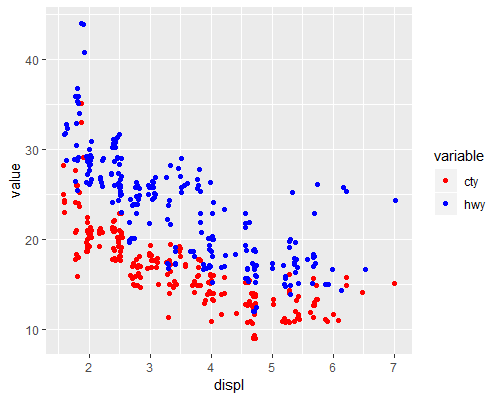
\includegraphics[width=3.64583in,height=\textheight]{images/06/ex6-4-2.png}

\begin{enumerate}
\def\labelenumi{\arabic{enumi})}
\setcounter{enumi}{3}
\tightlist
\item
  다음과 같이 배기량과 고속도로/도심 연비의 관계를 나타내는 추세선을 추가하시오 (\texttt{geom\_smooth} 이용)
\end{enumerate}

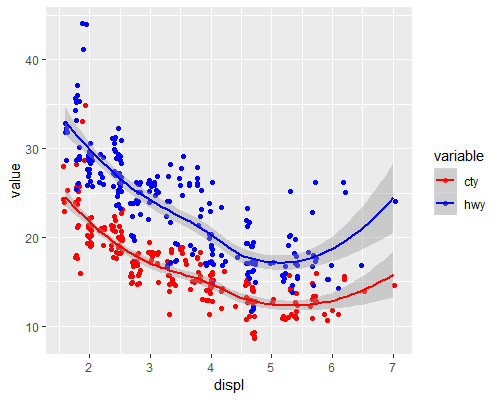
\includegraphics[width=3.64583in,height=\textheight]{images/06/ex6-4-4.png}

\begin{enumerate}
\def\labelenumi{\arabic{enumi})}
\setcounter{enumi}{4}
\tightlist
\item
  아래 그림과 같이 Theme을 \texttt{theme\_bw()}를 사용하고 추가로 Title, subtitle, x축, y축 라벨, 그리고 범례의 Title을 변경하시오. (범례의 라벨 설정은 \texttt{scale\_color\_manual}에서 \texttt{labels=c("City\ MPG",\ "Highway\ MPG")}으로 설정, 범례의 title을 지울때는 \texttt{name=element\_blank()}, Title의 택스트 크기는 20, x축, y축의 라벨 텍스트 크기는 18로 설정)
\end{enumerate}

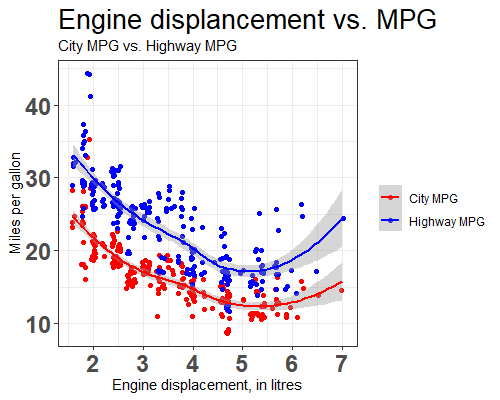
\includegraphics[width=3.64583in,height=\textheight]{images/06/ex6-4-5.png}

\hypertarget{ggplot-examples}{%
\section{ggplot examples}\label{ggplot-examples}}

인터넷에서 찾은 다음 사이트의 예제를 보면서 다양한 그래프 예제를 실행해 보겠습니다. 코드는 조금씩 변형된 부분이 있으니 참고 부탁 드립니다.

\begin{itemize}
\tightlist
\item
  \url{https://www.r-graph-gallery.com/ggplot2-package.html}
\item
  \url{http://r-statistics.co/Top50-Ggplot2-Visualizations-MasterList-R-Code.html}
\item
  \url{https://www.datanovia.com/en/blog/ggplot-examples-best-reference/}
\end{itemize}

\hypertarget{violin-plot}{%
\subsection{Violin plot}\label{violin-plot}}

\begin{itemize}
\tightlist
\item
  \url{https://www.r-graph-gallery.com/violin_and_boxplot_ggplot2.html}
\end{itemize}

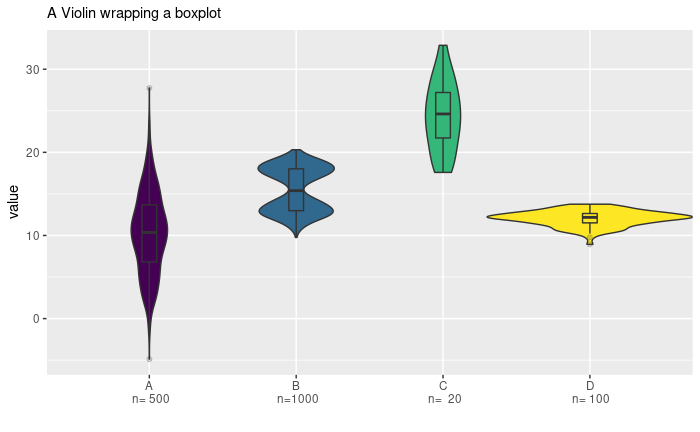
\includegraphics[width=4.6875in,height=\textheight]{images/10/000013.png}

\begin{Shaded}
\begin{Highlighting}[]
\FunctionTok{library}\NormalTok{(tidyverse)}
\FunctionTok{library}\NormalTok{(viridis)}

\CommentTok{\# create a dataset}
\NormalTok{data }\OtherTok{\textless{}{-}} \FunctionTok{data.frame}\NormalTok{(}
  \AttributeTok{name=}\FunctionTok{c}\NormalTok{( }\FunctionTok{rep}\NormalTok{(}\StringTok{"A"}\NormalTok{,}\DecValTok{500}\NormalTok{), }\FunctionTok{rep}\NormalTok{(}\StringTok{"B"}\NormalTok{,}\DecValTok{500}\NormalTok{), }\FunctionTok{rep}\NormalTok{(}\StringTok{"B"}\NormalTok{,}\DecValTok{500}\NormalTok{), }\FunctionTok{rep}\NormalTok{(}\StringTok{"C"}\NormalTok{,}\DecValTok{20}\NormalTok{), }\FunctionTok{rep}\NormalTok{(}\StringTok{\textquotesingle{}D\textquotesingle{}}\NormalTok{, }\DecValTok{100}\NormalTok{)  ),}
  \AttributeTok{value=}\FunctionTok{c}\NormalTok{( }\FunctionTok{rnorm}\NormalTok{(}\DecValTok{500}\NormalTok{, }\DecValTok{10}\NormalTok{, }\DecValTok{5}\NormalTok{), }\FunctionTok{rnorm}\NormalTok{(}\DecValTok{500}\NormalTok{, }\DecValTok{13}\NormalTok{, }\DecValTok{1}\NormalTok{), }\FunctionTok{rnorm}\NormalTok{(}\DecValTok{500}\NormalTok{, }\DecValTok{18}\NormalTok{, }\DecValTok{1}\NormalTok{), }\FunctionTok{rnorm}\NormalTok{(}\DecValTok{20}\NormalTok{, }\DecValTok{25}\NormalTok{, }\DecValTok{4}\NormalTok{), }\FunctionTok{rnorm}\NormalTok{(}\DecValTok{100}\NormalTok{, }\DecValTok{12}\NormalTok{, }\DecValTok{1}\NormalTok{) )}
\NormalTok{)}

\NormalTok{data }\SpecialCharTok{\%\textgreater{}\%}\NormalTok{ str}

\FunctionTok{ggplot}\NormalTok{(data, }\FunctionTok{aes}\NormalTok{(}\AttributeTok{x=}\NormalTok{name, }\AttributeTok{y=}\NormalTok{value, }\AttributeTok{fill=}\NormalTok{name)) }\SpecialCharTok{+}
    \FunctionTok{geom\_violin}\NormalTok{(}\AttributeTok{width=}\FloatTok{1.4}\NormalTok{) }\SpecialCharTok{+}
    \FunctionTok{geom\_boxplot}\NormalTok{(}\AttributeTok{width=}\FloatTok{0.1}\NormalTok{, }\AttributeTok{alpha=}\FloatTok{0.2}\NormalTok{) }

\CommentTok{\# sample summary}
\NormalTok{sample\_size }\OtherTok{=}\NormalTok{ data }\SpecialCharTok{\%\textgreater{}\%} 
  \FunctionTok{group\_by}\NormalTok{(name) }\SpecialCharTok{\%\textgreater{}\%} 
  \FunctionTok{summarize}\NormalTok{(}\AttributeTok{num=}\FunctionTok{n}\NormalTok{()) }

\NormalTok{xlab }\OtherTok{\textless{}{-}}\NormalTok{ sample\_size }\SpecialCharTok{\%\textgreater{}\%} 
  \FunctionTok{apply}\NormalTok{(}\DecValTok{1}\NormalTok{, }\ControlFlowTok{function}\NormalTok{(x)}\FunctionTok{paste0}\NormalTok{(x, }\AttributeTok{collapse=}\StringTok{"}\SpecialCharTok{\textbackslash{}n}\StringTok{ n="}\NormalTok{))}

\FunctionTok{apply}\NormalTok{(sample\_size, }\DecValTok{1}\NormalTok{, }\ControlFlowTok{function}\NormalTok{(x)}\FunctionTok{paste0}\NormalTok{(x, }\AttributeTok{collapse=}\StringTok{"}\SpecialCharTok{\textbackslash{}n}\StringTok{ n="}\NormalTok{))}

\FunctionTok{ggplot}\NormalTok{(data, }\FunctionTok{aes}\NormalTok{(}\AttributeTok{x=}\NormalTok{name, }\AttributeTok{y=}\NormalTok{value, }\AttributeTok{fill=}\NormalTok{name)) }\SpecialCharTok{+}
    \FunctionTok{geom\_violin}\NormalTok{(}\AttributeTok{width=}\FloatTok{1.4}\NormalTok{) }\SpecialCharTok{+}
    \FunctionTok{geom\_boxplot}\NormalTok{(}\AttributeTok{width=}\FloatTok{0.1}\NormalTok{, }\AttributeTok{alpha=}\FloatTok{0.2}\NormalTok{) }\SpecialCharTok{+}
    \FunctionTok{scale\_fill\_viridis}\NormalTok{(}\AttributeTok{discrete =} \ConstantTok{TRUE}\NormalTok{) }\SpecialCharTok{+}
    \FunctionTok{scale\_x\_discrete}\NormalTok{(}\AttributeTok{labels=}\NormalTok{xlab) }\SpecialCharTok{+}
    \FunctionTok{theme}\NormalTok{(}
      \AttributeTok{legend.position=}\StringTok{"none"}\NormalTok{,}
      \AttributeTok{plot.title =} \FunctionTok{element\_text}\NormalTok{(}\AttributeTok{size=}\DecValTok{11}\NormalTok{)}
\NormalTok{    ) }\SpecialCharTok{+}
    \FunctionTok{ggtitle}\NormalTok{(}\StringTok{"A Violin wrapping a boxplot"}\NormalTok{) }\SpecialCharTok{+}
    \FunctionTok{xlab}\NormalTok{(}\StringTok{""}\NormalTok{)}
\end{Highlighting}
\end{Shaded}

\hypertarget{bubble-plot}{%
\subsection{Bubble plot}\label{bubble-plot}}

\begin{itemize}
\tightlist
\item
  \url{https://www.r-graph-gallery.com/320-the-basis-of-bubble-plot.html}
\end{itemize}

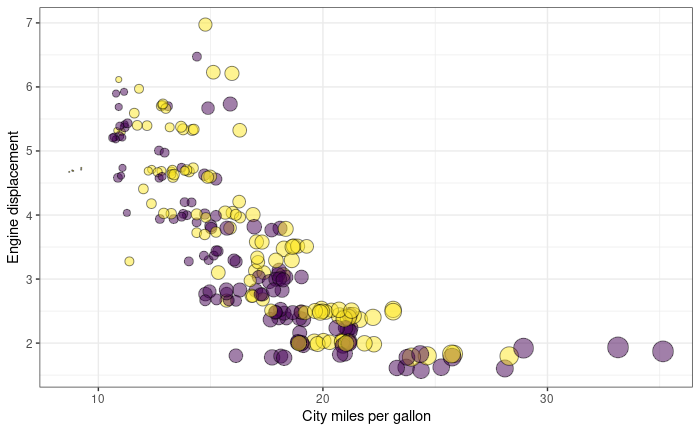
\includegraphics[width=4.6875in,height=\textheight]{images/10/000049.png}

\begin{Shaded}
\begin{Highlighting}[]
\NormalTok{mpg }\SpecialCharTok{\%\textgreater{}\%}\NormalTok{ str}

\CommentTok{\# Most basic bubble plot}
\FunctionTok{ggplot}\NormalTok{(mpg, }\FunctionTok{aes}\NormalTok{(}\AttributeTok{x=}\NormalTok{cty, }\AttributeTok{y=}\NormalTok{displ, }\AttributeTok{size =}\NormalTok{ hwy)) }\SpecialCharTok{+}
  \FunctionTok{geom\_point}\NormalTok{(}\AttributeTok{alpha=}\FloatTok{0.7}\NormalTok{, }\AttributeTok{position=}\StringTok{"jitter"}\NormalTok{) }
\end{Highlighting}
\end{Shaded}

\begin{Shaded}
\begin{Highlighting}[]
\FunctionTok{ggplot}\NormalTok{(mpg, }\FunctionTok{aes}\NormalTok{(}\AttributeTok{x=}\NormalTok{cty, }\AttributeTok{y=}\NormalTok{displ, }\AttributeTok{size =}\NormalTok{ hwy)) }\SpecialCharTok{+}
  \FunctionTok{geom\_point}\NormalTok{(}\AttributeTok{alpha=}\FloatTok{0.3}\NormalTok{, }\AttributeTok{position=}\StringTok{"jitter"}\NormalTok{) }\SpecialCharTok{+}
  \FunctionTok{scale\_size}\NormalTok{(}\AttributeTok{range =} \FunctionTok{c}\NormalTok{(.}\DecValTok{1}\NormalTok{, }\DecValTok{7}\NormalTok{), }\AttributeTok{name=}\StringTok{""}\NormalTok{)}
\end{Highlighting}
\end{Shaded}

\begin{Shaded}
\begin{Highlighting}[]
\FunctionTok{ggplot}\NormalTok{(mpg, }\FunctionTok{aes}\NormalTok{(}\AttributeTok{x=}\NormalTok{cty, }\AttributeTok{y=}\NormalTok{displ, }\AttributeTok{size =}\NormalTok{ hwy, }\AttributeTok{color=}\NormalTok{year)) }\SpecialCharTok{+}
  \FunctionTok{geom\_point}\NormalTok{(}\AttributeTok{alpha=}\FloatTok{0.3}\NormalTok{, }\AttributeTok{position=}\StringTok{"jitter"}\NormalTok{) }\SpecialCharTok{+}
  \FunctionTok{scale\_size}\NormalTok{(}\AttributeTok{range =} \FunctionTok{c}\NormalTok{(.}\DecValTok{1}\NormalTok{, }\DecValTok{7}\NormalTok{), }\AttributeTok{name=}\StringTok{""}\NormalTok{)}
\end{Highlighting}
\end{Shaded}

\begin{Shaded}
\begin{Highlighting}[]
\NormalTok{mpg }\SpecialCharTok{\%\textgreater{}\%} 
  \FunctionTok{mutate}\NormalTok{(}\AttributeTok{yearf =} \FunctionTok{factor}\NormalTok{(year)) }\SpecialCharTok{\%\textgreater{}\%} 
  \FunctionTok{ggplot}\NormalTok{(}\FunctionTok{aes}\NormalTok{(}\AttributeTok{x=}\NormalTok{cty, }\AttributeTok{y=}\NormalTok{displ, }\AttributeTok{size=}\NormalTok{hwy, }\AttributeTok{color=}\NormalTok{yearf)) }\SpecialCharTok{+}
  \FunctionTok{geom\_point}\NormalTok{(}\AttributeTok{alpha=}\FloatTok{0.3}\NormalTok{, }\AttributeTok{position=}\StringTok{"jitter"}\NormalTok{) }\SpecialCharTok{+}
  \FunctionTok{scale\_size}\NormalTok{(}\AttributeTok{range =} \FunctionTok{c}\NormalTok{(.}\DecValTok{1}\NormalTok{, }\DecValTok{7}\NormalTok{), }\AttributeTok{name=}\StringTok{""}\NormalTok{) }
\end{Highlighting}
\end{Shaded}

\begin{Shaded}
\begin{Highlighting}[]
\NormalTok{mpg }\SpecialCharTok{\%\textgreater{}\%} 
  \FunctionTok{mutate}\NormalTok{(}\AttributeTok{yearf =} \FunctionTok{factor}\NormalTok{(year)) }\SpecialCharTok{\%\textgreater{}\%} 
  \FunctionTok{ggplot}\NormalTok{(}\FunctionTok{aes}\NormalTok{(}\AttributeTok{x=}\NormalTok{cty, }\AttributeTok{y=}\NormalTok{displ, }\AttributeTok{size=}\NormalTok{hwy, }\AttributeTok{fill=}\NormalTok{yearf)) }\SpecialCharTok{+}
  \FunctionTok{geom\_point}\NormalTok{(}\AttributeTok{alpha=}\FloatTok{0.5}\NormalTok{, }\AttributeTok{position=}\StringTok{"jitter"}\NormalTok{, }\AttributeTok{shape=}\DecValTok{21}\NormalTok{) }\SpecialCharTok{+}
  \FunctionTok{scale\_size}\NormalTok{(}\AttributeTok{range =} \FunctionTok{c}\NormalTok{(.}\DecValTok{1}\NormalTok{, }\DecValTok{7}\NormalTok{), }\AttributeTok{name=}\StringTok{""}\NormalTok{) }\SpecialCharTok{+} 
  \FunctionTok{scale\_fill\_viridis}\NormalTok{(}\AttributeTok{discrete=}\ConstantTok{TRUE}\NormalTok{, }\AttributeTok{guide=}\ConstantTok{FALSE}\NormalTok{, }\AttributeTok{option=}\StringTok{"D"}\NormalTok{) }\SpecialCharTok{+}
  \FunctionTok{theme\_bw}\NormalTok{() }\SpecialCharTok{+}
  \FunctionTok{ylab}\NormalTok{(}\StringTok{"Engine displacement"}\NormalTok{) }\SpecialCharTok{+}
  \FunctionTok{xlab}\NormalTok{(}\StringTok{"City miles per gallon"}\NormalTok{) }\SpecialCharTok{+}
  \FunctionTok{theme}\NormalTok{(}\AttributeTok{legend.position =} \StringTok{"none"}\NormalTok{)}
\end{Highlighting}
\end{Shaded}

\hypertarget{barplot-with-errorbars}{%
\subsection{Barplot with errorbars}\label{barplot-with-errorbars}}

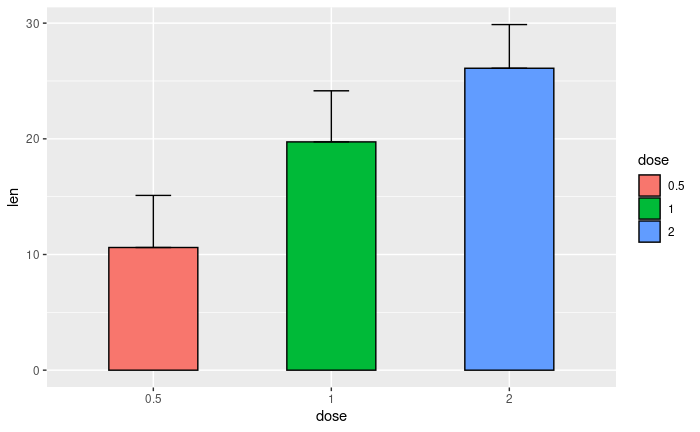
\includegraphics[width=4.6875in,height=\textheight]{images/10/00000e.png}

\begin{Shaded}
\begin{Highlighting}[]
\NormalTok{ToothGrowth }\SpecialCharTok{\%\textgreater{}\%}\NormalTok{ str}

\NormalTok{df }\OtherTok{\textless{}{-}}\NormalTok{ ToothGrowth }\SpecialCharTok{\%\textgreater{}\%} 
  \FunctionTok{mutate}\NormalTok{(}\AttributeTok{dose =} \FunctionTok{as.factor}\NormalTok{(dose))}
\NormalTok{df }\SpecialCharTok{\%\textgreater{}\%}\NormalTok{ str}

\DocumentationTok{\#\# summary}
\NormalTok{df\_summary }\OtherTok{\textless{}{-}}\NormalTok{ df }\SpecialCharTok{\%\textgreater{}\%}
  \FunctionTok{group\_by}\NormalTok{(dose) }\SpecialCharTok{\%\textgreater{}\%}
  \FunctionTok{summarise}\NormalTok{(}\AttributeTok{sd =} \FunctionTok{sd}\NormalTok{(len, }\AttributeTok{na.rm =} \ConstantTok{TRUE}\NormalTok{), }\AttributeTok{len =} \FunctionTok{mean}\NormalTok{(len))}
\NormalTok{df\_summary}


\FunctionTok{ggplot}\NormalTok{(df\_summary, }\FunctionTok{aes}\NormalTok{(}\AttributeTok{x=}\NormalTok{dose, }\AttributeTok{y=}\NormalTok{len, }\AttributeTok{fill=}\NormalTok{dose)) }\SpecialCharTok{+}
  \FunctionTok{geom\_bar}\NormalTok{(}\AttributeTok{stat =} \StringTok{"identity"}\NormalTok{, }\AttributeTok{color =} \StringTok{"black"}\NormalTok{, }\AttributeTok{width =} \FloatTok{0.5}\NormalTok{) }\SpecialCharTok{+}
  \FunctionTok{geom\_errorbar}\NormalTok{(}\FunctionTok{aes}\NormalTok{(}\AttributeTok{ymin =}\NormalTok{ len, }\AttributeTok{ymax =}\NormalTok{ len}\SpecialCharTok{+}\NormalTok{sd), }\AttributeTok{width =} \FloatTok{0.2}\NormalTok{) }
\end{Highlighting}
\end{Shaded}

\hypertarget{horizontal-barplot}{%
\subsection{horizontal barplot}\label{horizontal-barplot}}

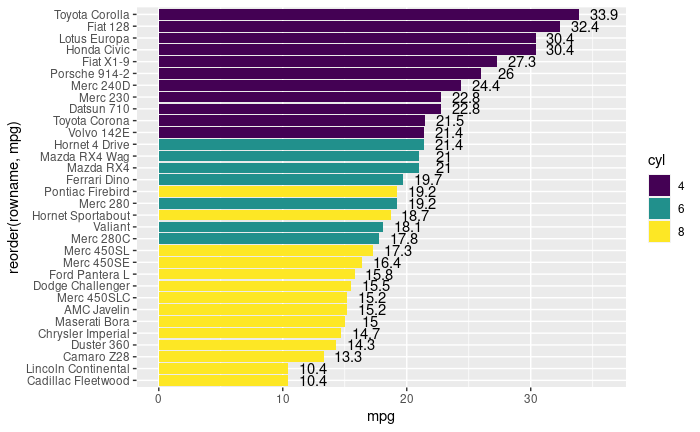
\includegraphics[width=4.6875in,height=\textheight]{images/10/00000b.png}

\begin{Shaded}
\begin{Highlighting}[]
\NormalTok{df }\OtherTok{\textless{}{-}}\NormalTok{ mtcars }\SpecialCharTok{\%\textgreater{}\%}
  \FunctionTok{rownames\_to\_column}\NormalTok{() }\SpecialCharTok{\%\textgreater{}\%}
  \FunctionTok{as\_data\_frame}\NormalTok{() }\SpecialCharTok{\%\textgreater{}\%}
  \FunctionTok{mutate}\NormalTok{(}\AttributeTok{cyl =} \FunctionTok{as.factor}\NormalTok{(cyl)) }\SpecialCharTok{\%\textgreater{}\%}
  \FunctionTok{select}\NormalTok{(rowname, wt, mpg, cyl)}
\NormalTok{df}

\CommentTok{\# change fill color by groups and add text labels}
\FunctionTok{ggplot}\NormalTok{(df, }\FunctionTok{aes}\NormalTok{(}\AttributeTok{x =} \FunctionTok{reorder}\NormalTok{(rowname, mpg), }\AttributeTok{y =}\NormalTok{ mpg)) }\SpecialCharTok{+}
  \FunctionTok{geom\_col}\NormalTok{(}\FunctionTok{aes}\NormalTok{(}\AttributeTok{fill =}\NormalTok{ cyl)) }\SpecialCharTok{+} 
  \FunctionTok{geom\_text}\NormalTok{(}\FunctionTok{aes}\NormalTok{(}\AttributeTok{label =}\NormalTok{ mpg), }\AttributeTok{nudge\_y =} \DecValTok{2}\NormalTok{) }\SpecialCharTok{+} 
  \FunctionTok{coord\_flip}\NormalTok{() }\SpecialCharTok{+}
  \FunctionTok{scale\_fill\_viridis\_d}\NormalTok{()}
\end{Highlighting}
\end{Shaded}

\hypertarget{circular-barplot}{%
\subsection{Circular barplot}\label{circular-barplot}}

\begin{itemize}
\tightlist
\item
  \url{https://www.r-graph-gallery.com/297-circular-barplot-with-groups.html}
\end{itemize}

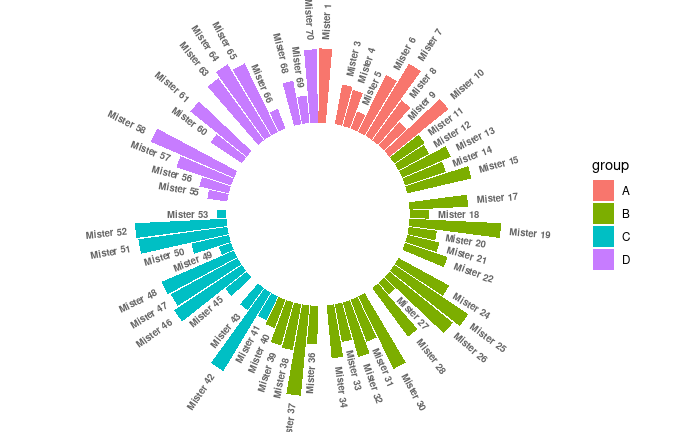
\includegraphics[width=4.6875in,height=\textheight]{images/10/000002.png}

\begin{Shaded}
\begin{Highlighting}[]
\CommentTok{\# Create dataset}
\NormalTok{n }\OtherTok{\textless{}{-}} \DecValTok{70}
\NormalTok{data }\OtherTok{\textless{}{-}} \FunctionTok{data.frame}\NormalTok{(}
  \AttributeTok{id =} \FunctionTok{seq}\NormalTok{(}\DecValTok{1}\NormalTok{, n),}
  \AttributeTok{individual=}\FunctionTok{paste}\NormalTok{( }\StringTok{"Mister "}\NormalTok{, }\FunctionTok{seq}\NormalTok{(}\DecValTok{1}\NormalTok{,n), }\AttributeTok{sep=}\StringTok{""}\NormalTok{),}
  \AttributeTok{group=}\FunctionTok{c}\NormalTok{( }\FunctionTok{rep}\NormalTok{(}\StringTok{\textquotesingle{}A\textquotesingle{}}\NormalTok{, }\DecValTok{10}\NormalTok{), }\FunctionTok{rep}\NormalTok{(}\StringTok{\textquotesingle{}B\textquotesingle{}}\NormalTok{, }\DecValTok{30}\NormalTok{), }\FunctionTok{rep}\NormalTok{(}\StringTok{\textquotesingle{}C\textquotesingle{}}\NormalTok{, }\DecValTok{14}\NormalTok{), }\FunctionTok{rep}\NormalTok{(}\StringTok{\textquotesingle{}D\textquotesingle{}}\NormalTok{, n}\DecValTok{{-}10{-}30{-}14}\NormalTok{)) ,}
  \AttributeTok{value=}\FunctionTok{sample}\NormalTok{( }\FunctionTok{seq}\NormalTok{(}\DecValTok{10}\NormalTok{,}\DecValTok{100}\NormalTok{), n, }\AttributeTok{replace=}\NormalTok{T)}
\NormalTok{)}
\NormalTok{data }\SpecialCharTok{\%\textgreater{}\%}\NormalTok{ str}

\CommentTok{\# introduce NA}
\NormalTok{empty\_bar\_idx }\OtherTok{\textless{}{-}} \FunctionTok{sample}\NormalTok{(}\DecValTok{1}\SpecialCharTok{:}\NormalTok{n, }\DecValTok{10}\NormalTok{)}
\NormalTok{data[empty\_bar\_idx,}\FunctionTok{c}\NormalTok{(}\DecValTok{2}\SpecialCharTok{:}\DecValTok{4}\NormalTok{)] }\OtherTok{\textless{}{-}} \FunctionTok{c}\NormalTok{(}\ConstantTok{NA}\NormalTok{, }\ConstantTok{NA}\NormalTok{, }\ConstantTok{NA}\NormalTok{)}

\NormalTok{label\_data }\OtherTok{\textless{}{-}}\NormalTok{ data}
\NormalTok{number\_of\_bar }\OtherTok{\textless{}{-}} \FunctionTok{nrow}\NormalTok{(label\_data)}
\NormalTok{angle }\OtherTok{\textless{}{-}} \DecValTok{90} \SpecialCharTok{{-}} \DecValTok{360} \SpecialCharTok{*}\NormalTok{ (label\_data}\SpecialCharTok{$}\NormalTok{id}\FloatTok{{-}0.5}\NormalTok{) }\SpecialCharTok{/}\NormalTok{number\_of\_bar     }\CommentTok{\# I substract 0.5 because the letter must have the angle of the center of the bars. Not extreme right(1) or extreme left (0)}
\NormalTok{label\_data}\SpecialCharTok{$}\NormalTok{hjust }\OtherTok{\textless{}{-}} \FunctionTok{ifelse}\NormalTok{( angle }\SpecialCharTok{\textless{}} \SpecialCharTok{{-}}\DecValTok{90}\NormalTok{, }\DecValTok{1}\NormalTok{, }\DecValTok{0}\NormalTok{)}
\NormalTok{label\_data}\SpecialCharTok{$}\NormalTok{angle }\OtherTok{\textless{}{-}} \FunctionTok{ifelse}\NormalTok{(angle }\SpecialCharTok{\textless{}} \SpecialCharTok{{-}}\DecValTok{90}\NormalTok{, angle}\SpecialCharTok{+}\DecValTok{180}\NormalTok{, angle)}

\NormalTok{data }\SpecialCharTok{\%\textgreater{}\%} 
\FunctionTok{ggplot}\NormalTok{(}\FunctionTok{aes}\NormalTok{(}\AttributeTok{x=}\FunctionTok{as.factor}\NormalTok{(id), }\AttributeTok{y=}\NormalTok{value, }\AttributeTok{fill=}\NormalTok{group)) }\SpecialCharTok{+}
  \FunctionTok{geom\_bar}\NormalTok{(}\AttributeTok{stat=}\StringTok{"identity"}\NormalTok{) }\SpecialCharTok{+}
  \FunctionTok{ylim}\NormalTok{(}\SpecialCharTok{{-}}\DecValTok{100}\NormalTok{,}\DecValTok{120}\NormalTok{) }\SpecialCharTok{+}
  \FunctionTok{theme\_minimal}\NormalTok{() }\SpecialCharTok{+}
  \FunctionTok{theme}\NormalTok{(}
    \AttributeTok{axis.text =} \FunctionTok{element\_blank}\NormalTok{(),}
    \AttributeTok{axis.title =} \FunctionTok{element\_blank}\NormalTok{(),}
    \AttributeTok{panel.grid =} \FunctionTok{element\_blank}\NormalTok{(),}
    \AttributeTok{plot.margin =} \FunctionTok{unit}\NormalTok{(}\FunctionTok{rep}\NormalTok{(}\SpecialCharTok{{-}}\DecValTok{1}\NormalTok{,}\DecValTok{4}\NormalTok{), }\StringTok{"cm"}\NormalTok{) }
\NormalTok{  ) }\SpecialCharTok{+}
  \FunctionTok{coord\_polar}\NormalTok{(}\AttributeTok{start =} \DecValTok{0}\NormalTok{) }\SpecialCharTok{+} 
  \FunctionTok{geom\_text}\NormalTok{(}\AttributeTok{data=}\NormalTok{label\_data, }\FunctionTok{aes}\NormalTok{(}\AttributeTok{x=}\NormalTok{id, }\AttributeTok{y=}\NormalTok{value}\SpecialCharTok{+}\DecValTok{10}\NormalTok{, }\AttributeTok{label=}\NormalTok{individual, }\AttributeTok{hjust=}\NormalTok{hjust), }\AttributeTok{color=}\StringTok{"black"}\NormalTok{, }\AttributeTok{fontface=}\StringTok{"bold"}\NormalTok{, }\AttributeTok{alpha=}\FloatTok{0.6}\NormalTok{, }\AttributeTok{size=}\FloatTok{2.5}\NormalTok{, }\AttributeTok{angle=}\NormalTok{ label\_data}\SpecialCharTok{$}\NormalTok{angle, }\AttributeTok{inherit.aes =} \ConstantTok{FALSE}\NormalTok{ ) }
\end{Highlighting}
\end{Shaded}

데이터 정렬 후 plot

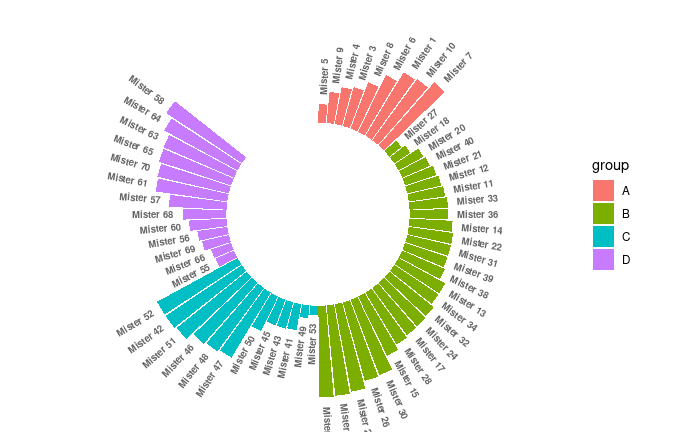
\includegraphics[width=4.6875in,height=\textheight]{images/10/000008.png}

\begin{Shaded}
\begin{Highlighting}[]
\NormalTok{data2 }\OtherTok{\textless{}{-}}\NormalTok{ data }\SpecialCharTok{\%\textgreater{}\%} 
  \FunctionTok{arrange}\NormalTok{(group, value) }\SpecialCharTok{\%\textgreater{}\%} 
  \FunctionTok{mutate}\NormalTok{(}\AttributeTok{id2=}\DecValTok{1}\SpecialCharTok{:}\FunctionTok{n}\NormalTok{()) }

\NormalTok{label\_data2 }\OtherTok{\textless{}{-}}\NormalTok{ data2}
\NormalTok{number\_of\_bar }\OtherTok{\textless{}{-}} \FunctionTok{nrow}\NormalTok{(label\_data2)}
\NormalTok{angle }\OtherTok{\textless{}{-}} \DecValTok{90} \SpecialCharTok{{-}} \DecValTok{360} \SpecialCharTok{*}\NormalTok{ (label\_data2}\SpecialCharTok{$}\NormalTok{id2}\FloatTok{{-}0.5}\NormalTok{) }\SpecialCharTok{/}\NormalTok{number\_of\_bar     }\CommentTok{\# I substract 0.5 because the letter must have the angle of the center of the bars. Not extreme right(1) or extreme left (0)}
\NormalTok{label\_data2}\SpecialCharTok{$}\NormalTok{hjust }\OtherTok{\textless{}{-}} \FunctionTok{ifelse}\NormalTok{( angle }\SpecialCharTok{\textless{}} \SpecialCharTok{{-}}\DecValTok{90}\NormalTok{, }\DecValTok{1}\NormalTok{, }\DecValTok{0}\NormalTok{)}
\NormalTok{label\_data2}\SpecialCharTok{$}\NormalTok{angle }\OtherTok{\textless{}{-}} \FunctionTok{ifelse}\NormalTok{(angle }\SpecialCharTok{\textless{}} \SpecialCharTok{{-}}\DecValTok{90}\NormalTok{, angle}\SpecialCharTok{+}\DecValTok{180}\NormalTok{, angle)}


\NormalTok{data2 }\SpecialCharTok{\%\textgreater{}\%} 
  \FunctionTok{ggplot}\NormalTok{(}\FunctionTok{aes}\NormalTok{(}\AttributeTok{x=}\FunctionTok{as.factor}\NormalTok{(id2), }\AttributeTok{y=}\NormalTok{value, }\AttributeTok{fill=}\NormalTok{group)) }\SpecialCharTok{+}
  \FunctionTok{geom\_bar}\NormalTok{(}\AttributeTok{stat=}\StringTok{"identity"}\NormalTok{) }\SpecialCharTok{+}
  \FunctionTok{ylim}\NormalTok{(}\SpecialCharTok{{-}}\DecValTok{100}\NormalTok{,}\DecValTok{120}\NormalTok{) }\SpecialCharTok{+}
  \FunctionTok{theme\_minimal}\NormalTok{() }\SpecialCharTok{+}
  \FunctionTok{theme}\NormalTok{(}
    \AttributeTok{axis.text =} \FunctionTok{element\_blank}\NormalTok{(),}
    \AttributeTok{axis.title =} \FunctionTok{element\_blank}\NormalTok{(),}
    \AttributeTok{panel.grid =} \FunctionTok{element\_blank}\NormalTok{(),}
    \AttributeTok{plot.margin =} \FunctionTok{unit}\NormalTok{(}\FunctionTok{rep}\NormalTok{(}\SpecialCharTok{{-}}\DecValTok{1}\NormalTok{,}\DecValTok{4}\NormalTok{), }\StringTok{"cm"}\NormalTok{) }
\NormalTok{  ) }\SpecialCharTok{+}
  \FunctionTok{coord\_polar}\NormalTok{(}\AttributeTok{start =} \DecValTok{0}\NormalTok{) }\SpecialCharTok{+} 
  \FunctionTok{geom\_text}\NormalTok{(}\AttributeTok{data=}\NormalTok{label\_data2, }\FunctionTok{aes}\NormalTok{(}\AttributeTok{x=}\NormalTok{id2, }\AttributeTok{y=}\NormalTok{value}\SpecialCharTok{+}\DecValTok{10}\NormalTok{, }\AttributeTok{label=}\NormalTok{individual, }\AttributeTok{hjust=}\NormalTok{hjust), }\AttributeTok{color=}\StringTok{"black"}\NormalTok{, }\AttributeTok{fontface=}\StringTok{"bold"}\NormalTok{,}\AttributeTok{alpha=}\FloatTok{0.6}\NormalTok{, }\AttributeTok{size=}\FloatTok{2.5}\NormalTok{, }\AttributeTok{angle=}\NormalTok{ label\_data}\SpecialCharTok{$}\NormalTok{angle, }\AttributeTok{inherit.aes =} \ConstantTok{FALSE}\NormalTok{ ) }
\end{Highlighting}
\end{Shaded}

\hypertarget{stacked-area-chart}{%
\subsection{Stacked area chart}\label{stacked-area-chart}}

\begin{itemize}
\tightlist
\item
  \url{https://www.data-to-viz.com/caveat/stacking.html}
\end{itemize}

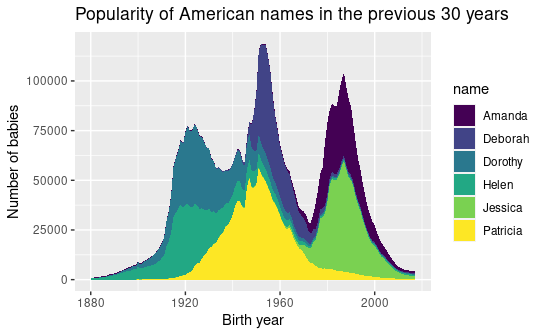
\includegraphics[width=4.6875in,height=\textheight]{images/10/000009a.png}

\begin{Shaded}
\begin{Highlighting}[]
\FunctionTok{library}\NormalTok{(babynames)}

\NormalTok{babynames }\SpecialCharTok{\%\textgreater{}\%}\NormalTok{ str}


\CommentTok{\# Load dataset from github}
\NormalTok{data }\OtherTok{\textless{}{-}}\NormalTok{ babynames }\SpecialCharTok{\%\textgreater{}\%} 
  \FunctionTok{filter}\NormalTok{(name }\SpecialCharTok{\%in\%} \FunctionTok{c}\NormalTok{(}\StringTok{"Amanda"}\NormalTok{, }\StringTok{"Jessica"}\NormalTok{,    }\StringTok{"Patricia"}\NormalTok{, }\StringTok{"Deborah"}\NormalTok{,   }\StringTok{"Dorothy"}\NormalTok{,  }\StringTok{"Helen"}\NormalTok{)) }\SpecialCharTok{\%\textgreater{}\%}
  \FunctionTok{filter}\NormalTok{(sex}\SpecialCharTok{==}\StringTok{"F"}\NormalTok{)}

\CommentTok{\# Plot}
\NormalTok{p }\OtherTok{\textless{}{-}}\NormalTok{ data }\SpecialCharTok{\%\textgreater{}\%} 
  \FunctionTok{ggplot}\NormalTok{(}\FunctionTok{aes}\NormalTok{(}\AttributeTok{x=}\NormalTok{year, }\AttributeTok{y=}\NormalTok{n, }\AttributeTok{fill=}\NormalTok{name, }\AttributeTok{text=}\NormalTok{name)) }\SpecialCharTok{+}
    \FunctionTok{geom\_area}\NormalTok{( ) }\SpecialCharTok{+}
    \FunctionTok{scale\_fill\_viridis}\NormalTok{(}\AttributeTok{discrete =} \ConstantTok{TRUE}\NormalTok{) }\SpecialCharTok{+}
    \FunctionTok{ggtitle}\NormalTok{(}\StringTok{"Popularity of American names in the previous 30 years"}\NormalTok{) }\SpecialCharTok{+}
    \FunctionTok{theme}\NormalTok{() }\SpecialCharTok{+}
    \FunctionTok{xlab}\NormalTok{(}\StringTok{"Birth year"}\NormalTok{) }\SpecialCharTok{+}
    \FunctionTok{ylab}\NormalTok{(}\StringTok{"Number of babies"}\NormalTok{)}
\NormalTok{p}
\end{Highlighting}
\end{Shaded}

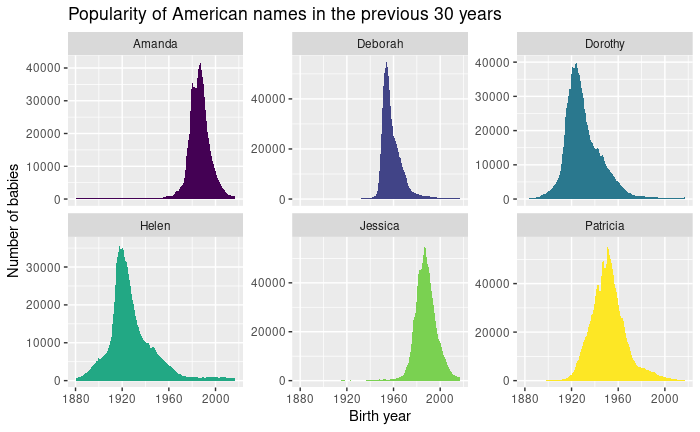
\includegraphics[width=4.6875in,height=\textheight]{images/10/000006.png}

\begin{Shaded}
\begin{Highlighting}[]
\NormalTok{p }\SpecialCharTok{+} \FunctionTok{facet\_wrap}\NormalTok{(}\SpecialCharTok{\textasciitilde{}}\NormalTok{name, }\AttributeTok{scale=}\StringTok{"free\_y"}\NormalTok{)}
\end{Highlighting}
\end{Shaded}

\hypertarget{density-plot}{%
\subsection{Density plot}\label{density-plot}}

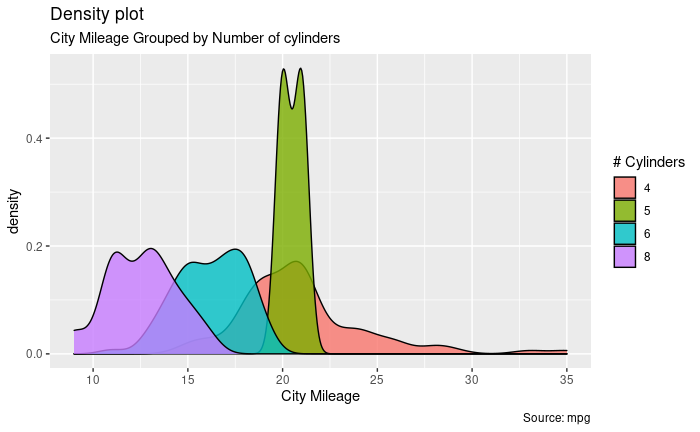
\includegraphics[width=4.6875in,height=\textheight]{images/10/000003.png}

\begin{Shaded}
\begin{Highlighting}[]
\CommentTok{\# Plot}
\NormalTok{g }\OtherTok{\textless{}{-}} \FunctionTok{ggplot}\NormalTok{(mpg, }\FunctionTok{aes}\NormalTok{(cty))}
\NormalTok{g }\SpecialCharTok{+} \FunctionTok{geom\_density}\NormalTok{(}\FunctionTok{aes}\NormalTok{(}\AttributeTok{fill=}\FunctionTok{factor}\NormalTok{(cyl)), }\AttributeTok{alpha=}\FloatTok{0.8}\NormalTok{) }\SpecialCharTok{+} 
    \FunctionTok{labs}\NormalTok{(}\AttributeTok{title=}\StringTok{"Density plot"}\NormalTok{, }
         \AttributeTok{subtitle=}\StringTok{"City Mileage Grouped by Number of cylinders"}\NormalTok{,}
         \AttributeTok{caption=}\StringTok{"Source: mpg"}\NormalTok{,}
         \AttributeTok{x=}\StringTok{"City Mileage"}\NormalTok{,}
         \AttributeTok{fill=}\StringTok{"\# Cylinders"}\NormalTok{)}
\end{Highlighting}
\end{Shaded}

\hypertarget{waffle-chart}{%
\subsection{Waffle chart}\label{waffle-chart}}

\begin{itemize}
\tightlist
\item
  \url{http://r-statistics.co/Top50-Ggplot2-Visualizations-MasterList-R-Code.html\#Waffle\%20Chart}
\end{itemize}

\begin{Shaded}
\begin{Highlighting}[]
\NormalTok{var }\OtherTok{\textless{}{-}}\NormalTok{ mpg}\SpecialCharTok{$}\NormalTok{class  }\CommentTok{\# the categorical data }

\DocumentationTok{\#\# Prep data (nothing to change here)}
\NormalTok{nrows }\OtherTok{\textless{}{-}} \DecValTok{10}
\NormalTok{df }\OtherTok{\textless{}{-}} \FunctionTok{expand.grid}\NormalTok{(}\AttributeTok{y =} \DecValTok{1}\SpecialCharTok{:}\NormalTok{nrows, }\AttributeTok{x =} \DecValTok{1}\SpecialCharTok{:}\NormalTok{nrows)}
\NormalTok{categ\_table }\OtherTok{\textless{}{-}} \FunctionTok{round}\NormalTok{(}\FunctionTok{table}\NormalTok{(var) }\SpecialCharTok{*}\NormalTok{ ((nrows}\SpecialCharTok{*}\NormalTok{nrows)}\SpecialCharTok{/}\NormalTok{(}\FunctionTok{length}\NormalTok{(var))))}
\NormalTok{categ\_table}


\NormalTok{df}\SpecialCharTok{$}\NormalTok{category }\OtherTok{\textless{}{-}} \FunctionTok{factor}\NormalTok{(}\FunctionTok{rep}\NormalTok{(}\FunctionTok{names}\NormalTok{(categ\_table), categ\_table))  }
\CommentTok{\# }\AlertTok{NOTE}\CommentTok{: if sum(categ\_table) is not 100 (i.e. nrows\^{}2), it will need adjustment to make the sum to 100.}

\DocumentationTok{\#\# Plot}
\NormalTok{df }\SpecialCharTok{\%\textgreater{}\%}\NormalTok{ str}
\FunctionTok{ggplot}\NormalTok{(df, }\FunctionTok{aes}\NormalTok{(}\AttributeTok{x =}\NormalTok{ x, }\AttributeTok{y =}\NormalTok{ y, }\AttributeTok{fill =}\NormalTok{ category)) }\SpecialCharTok{+} 
        \FunctionTok{geom\_tile}\NormalTok{(}\AttributeTok{color =} \StringTok{"black"}\NormalTok{, }\AttributeTok{size =} \FloatTok{0.5}\NormalTok{) }
\end{Highlighting}
\end{Shaded}

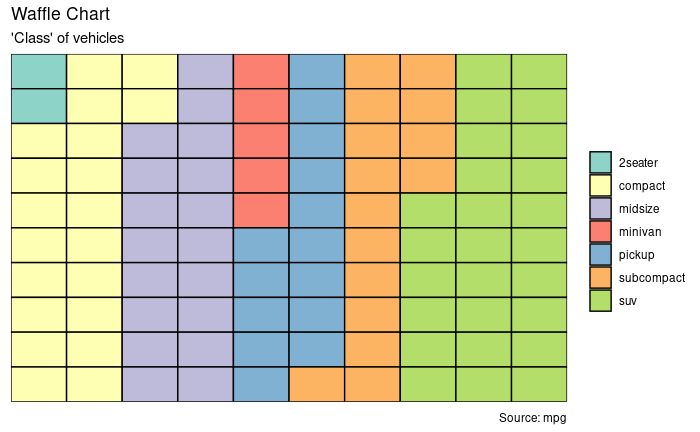
\includegraphics[width=4.6875in,height=\textheight]{images/10/00000a.png}

\begin{Shaded}
\begin{Highlighting}[]
\FunctionTok{ggplot}\NormalTok{(df, }\FunctionTok{aes}\NormalTok{(}\AttributeTok{x =}\NormalTok{ x, }\AttributeTok{y =}\NormalTok{ y, }\AttributeTok{fill =}\NormalTok{ category)) }\SpecialCharTok{+} 
        \FunctionTok{geom\_tile}\NormalTok{(}\AttributeTok{color =} \StringTok{"black"}\NormalTok{, }\AttributeTok{size =} \FloatTok{0.5}\NormalTok{) }\SpecialCharTok{+}
        \FunctionTok{scale\_x\_continuous}\NormalTok{(}\AttributeTok{expand =} \FunctionTok{c}\NormalTok{(}\DecValTok{0}\NormalTok{, }\DecValTok{0}\NormalTok{)) }\SpecialCharTok{+}
        \FunctionTok{scale\_y\_continuous}\NormalTok{(}\AttributeTok{expand =} \FunctionTok{c}\NormalTok{(}\DecValTok{0}\NormalTok{, }\DecValTok{0}\NormalTok{), }\AttributeTok{trans =} \StringTok{\textquotesingle{}reverse\textquotesingle{}}\NormalTok{) }\SpecialCharTok{+}
        \FunctionTok{scale\_fill\_brewer}\NormalTok{(}\AttributeTok{palette =} \StringTok{"Set3"}\NormalTok{) }\SpecialCharTok{+}
        \FunctionTok{labs}\NormalTok{(}\AttributeTok{title=}\StringTok{"Waffle Chart"}\NormalTok{, }\AttributeTok{subtitle=}\StringTok{"\textquotesingle{}Class\textquotesingle{} of vehicles"}\NormalTok{,}
             \AttributeTok{caption=}\StringTok{"Source: mpg"}\NormalTok{) }\SpecialCharTok{+} 
        \FunctionTok{theme}\NormalTok{(}\AttributeTok{plot.title =} \FunctionTok{element\_text}\NormalTok{(}\AttributeTok{size =} \FunctionTok{rel}\NormalTok{(}\FloatTok{1.2}\NormalTok{)),}
              \AttributeTok{axis.text =} \FunctionTok{element\_blank}\NormalTok{(),}
              \AttributeTok{axis.title =} \FunctionTok{element\_blank}\NormalTok{(),}
              \AttributeTok{axis.ticks =} \FunctionTok{element\_blank}\NormalTok{(),}
              \AttributeTok{legend.title =} \FunctionTok{element\_blank}\NormalTok{(),}
              \AttributeTok{legend.position =} \StringTok{"right"}\NormalTok{)}
\end{Highlighting}
\end{Shaded}

\hypertarget{marginal-histogram}{%
\subsection{Marginal histogram}\label{marginal-histogram}}

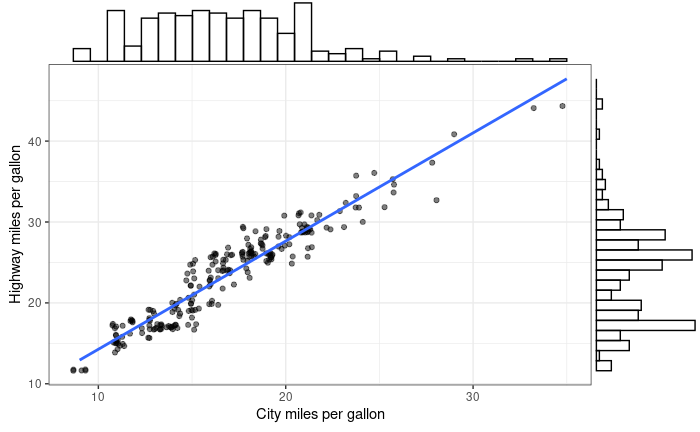
\includegraphics[width=4.6875in,height=\textheight]{images/10/000046.png}

\begin{Shaded}
\begin{Highlighting}[]
\FunctionTok{library}\NormalTok{(ggExtra)}

\CommentTok{\# Scatterplot}
\NormalTok{p }\OtherTok{\textless{}{-}} \FunctionTok{ggplot}\NormalTok{(mpg, }\FunctionTok{aes}\NormalTok{(}\AttributeTok{x=}\NormalTok{cty, }\AttributeTok{y=}\NormalTok{hwy)) }\SpecialCharTok{+} 
  \FunctionTok{geom\_point}\NormalTok{(}\AttributeTok{position=}\StringTok{"jitter"}\NormalTok{, }\AttributeTok{alpha=}\FloatTok{0.5}\NormalTok{) }\SpecialCharTok{+}
  \FunctionTok{geom\_smooth}\NormalTok{(}\AttributeTok{method=}\StringTok{"lm"}\NormalTok{, }\AttributeTok{se=}\NormalTok{F) }\SpecialCharTok{+}
  \FunctionTok{theme\_bw}\NormalTok{() }\SpecialCharTok{+}
  \FunctionTok{theme}\NormalTok{(}
    \AttributeTok{legend.position =} \StringTok{"none"}
\NormalTok{  ) }\SpecialCharTok{+}
  \FunctionTok{xlab}\NormalTok{(}\StringTok{"City miles per gallon"}\NormalTok{) }\SpecialCharTok{+}
  \FunctionTok{ylab}\NormalTok{(}\StringTok{"Highway miles per gallon"}\NormalTok{)}
\NormalTok{p}
\FunctionTok{ggMarginal}\NormalTok{(p, }\AttributeTok{type =} \StringTok{"histogram"}\NormalTok{, }\AttributeTok{fill=}\StringTok{"transparent"}\NormalTok{) }
\FunctionTok{ggMarginal}\NormalTok{(p, }\AttributeTok{type =} \StringTok{"density"}\NormalTok{, }\AttributeTok{fill=}\StringTok{"transparent"}\NormalTok{)}
\end{Highlighting}
\end{Shaded}

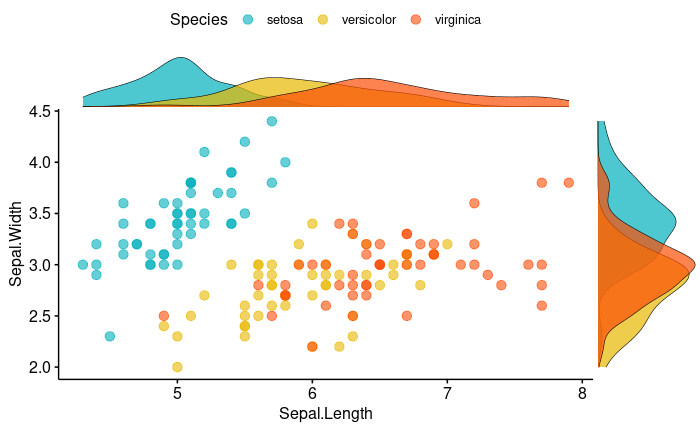
\includegraphics[width=4.6875in,height=\textheight]{images/10/000005.png}

\begin{Shaded}
\begin{Highlighting}[]
\FunctionTok{library}\NormalTok{(ggpubr)}
\CommentTok{\# Grouped Scatter plot with marginal density plots}
\FunctionTok{ggscatterhist}\NormalTok{(}
\NormalTok{  iris, }
  \AttributeTok{x =} \StringTok{"Sepal.Length"}\NormalTok{, }
  \AttributeTok{y =} \StringTok{"Sepal.Width"}\NormalTok{,}
  \AttributeTok{color =} \StringTok{"Species"}\NormalTok{, }
  \AttributeTok{size =} \DecValTok{3}\NormalTok{, }
  \AttributeTok{alpha =} \FloatTok{0.6}\NormalTok{,}
  \AttributeTok{palette =} \FunctionTok{c}\NormalTok{(}\StringTok{"\#00AFBB"}\NormalTok{, }\StringTok{"\#E7B800"}\NormalTok{, }\StringTok{"\#FC4E07"}\NormalTok{),}
  \AttributeTok{margin.params =} \FunctionTok{list}\NormalTok{(}\AttributeTok{fill =} \StringTok{"Species"}\NormalTok{, }\AttributeTok{color =} \StringTok{"black"}\NormalTok{, }\AttributeTok{size =} \FloatTok{0.2}\NormalTok{)}
\NormalTok{  )}
\end{Highlighting}
\end{Shaded}

\hypertarget{density-ridgeline-plots}{%
\subsection{Density ridgeline plots}\label{density-ridgeline-plots}}

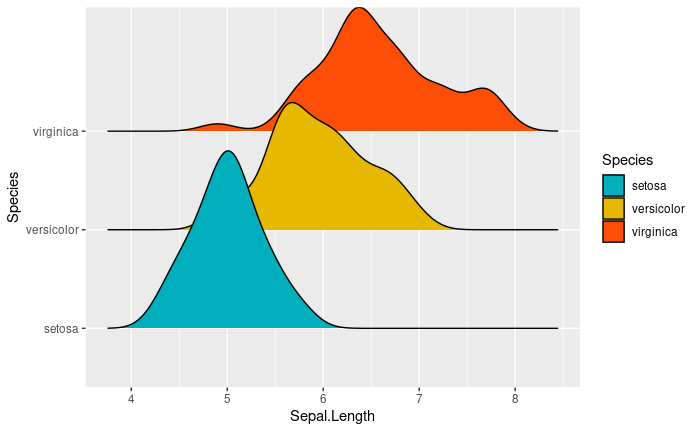
\includegraphics[width=4.6875in,height=\textheight]{images/10/000004.png}

\begin{Shaded}
\begin{Highlighting}[]
\FunctionTok{library}\NormalTok{(ggridges)}
\FunctionTok{ggplot}\NormalTok{(iris, }\FunctionTok{aes}\NormalTok{(}\AttributeTok{x =}\NormalTok{ Sepal.Length, }\AttributeTok{y =}\NormalTok{ Species)) }\SpecialCharTok{+}
  \FunctionTok{geom\_density\_ridges}\NormalTok{(}\FunctionTok{aes}\NormalTok{(}\AttributeTok{fill =}\NormalTok{ Species)) }\SpecialCharTok{+}
  \FunctionTok{scale\_fill\_manual}\NormalTok{(}\AttributeTok{values =} \FunctionTok{c}\NormalTok{(}\StringTok{"\#00AFBB"}\NormalTok{, }\StringTok{"\#E7B800"}\NormalTok{, }\StringTok{"\#FC4E07"}\NormalTok{))}
\end{Highlighting}
\end{Shaded}

\begin{center}\rule{0.5\linewidth}{0.5pt}\end{center}

이 저작물은 크리에이티브 커먼즈 저작자표시-비영리-변경금지 4.0 국제 라이선스에 따라 이용할 수 있습니다.

\end{document}
